% Options for packages loaded elsewhere
\PassOptionsToPackage{unicode}{hyperref}
\PassOptionsToPackage{hyphens}{url}
%
\documentclass[
]{book}
\usepackage{amsmath,amssymb}
\usepackage{iftex}
\ifPDFTeX
  \usepackage[T1]{fontenc}
  \usepackage[utf8]{inputenc}
  \usepackage{textcomp} % provide euro and other symbols
\else % if luatex or xetex
  \usepackage{unicode-math} % this also loads fontspec
  \defaultfontfeatures{Scale=MatchLowercase}
  \defaultfontfeatures[\rmfamily]{Ligatures=TeX,Scale=1}
\fi
\usepackage{lmodern}
\ifPDFTeX\else
  % xetex/luatex font selection
\fi
% Use upquote if available, for straight quotes in verbatim environments
\IfFileExists{upquote.sty}{\usepackage{upquote}}{}
\IfFileExists{microtype.sty}{% use microtype if available
  \usepackage[]{microtype}
  \UseMicrotypeSet[protrusion]{basicmath} % disable protrusion for tt fonts
}{}
\makeatletter
\@ifundefined{KOMAClassName}{% if non-KOMA class
  \IfFileExists{parskip.sty}{%
    \usepackage{parskip}
  }{% else
    \setlength{\parindent}{0pt}
    \setlength{\parskip}{6pt plus 2pt minus 1pt}}
}{% if KOMA class
  \KOMAoptions{parskip=half}}
\makeatother
\usepackage{xcolor}
\usepackage{color}
\usepackage{fancyvrb}
\newcommand{\VerbBar}{|}
\newcommand{\VERB}{\Verb[commandchars=\\\{\}]}
\DefineVerbatimEnvironment{Highlighting}{Verbatim}{commandchars=\\\{\}}
% Add ',fontsize=\small' for more characters per line
\usepackage{framed}
\definecolor{shadecolor}{RGB}{248,248,248}
\newenvironment{Shaded}{\begin{snugshade}}{\end{snugshade}}
\newcommand{\AlertTok}[1]{\textcolor[rgb]{0.94,0.16,0.16}{#1}}
\newcommand{\AnnotationTok}[1]{\textcolor[rgb]{0.56,0.35,0.01}{\textbf{\textit{#1}}}}
\newcommand{\AttributeTok}[1]{\textcolor[rgb]{0.77,0.63,0.00}{#1}}
\newcommand{\BaseNTok}[1]{\textcolor[rgb]{0.00,0.00,0.81}{#1}}
\newcommand{\BuiltInTok}[1]{#1}
\newcommand{\CharTok}[1]{\textcolor[rgb]{0.31,0.60,0.02}{#1}}
\newcommand{\CommentTok}[1]{\textcolor[rgb]{0.56,0.35,0.01}{\textit{#1}}}
\newcommand{\CommentVarTok}[1]{\textcolor[rgb]{0.56,0.35,0.01}{\textbf{\textit{#1}}}}
\newcommand{\ConstantTok}[1]{\textcolor[rgb]{0.00,0.00,0.00}{#1}}
\newcommand{\ControlFlowTok}[1]{\textcolor[rgb]{0.13,0.29,0.53}{\textbf{#1}}}
\newcommand{\DataTypeTok}[1]{\textcolor[rgb]{0.13,0.29,0.53}{#1}}
\newcommand{\DecValTok}[1]{\textcolor[rgb]{0.00,0.00,0.81}{#1}}
\newcommand{\DocumentationTok}[1]{\textcolor[rgb]{0.56,0.35,0.01}{\textbf{\textit{#1}}}}
\newcommand{\ErrorTok}[1]{\textcolor[rgb]{0.64,0.00,0.00}{\textbf{#1}}}
\newcommand{\ExtensionTok}[1]{#1}
\newcommand{\FloatTok}[1]{\textcolor[rgb]{0.00,0.00,0.81}{#1}}
\newcommand{\FunctionTok}[1]{\textcolor[rgb]{0.00,0.00,0.00}{#1}}
\newcommand{\ImportTok}[1]{#1}
\newcommand{\InformationTok}[1]{\textcolor[rgb]{0.56,0.35,0.01}{\textbf{\textit{#1}}}}
\newcommand{\KeywordTok}[1]{\textcolor[rgb]{0.13,0.29,0.53}{\textbf{#1}}}
\newcommand{\NormalTok}[1]{#1}
\newcommand{\OperatorTok}[1]{\textcolor[rgb]{0.81,0.36,0.00}{\textbf{#1}}}
\newcommand{\OtherTok}[1]{\textcolor[rgb]{0.56,0.35,0.01}{#1}}
\newcommand{\PreprocessorTok}[1]{\textcolor[rgb]{0.56,0.35,0.01}{\textit{#1}}}
\newcommand{\RegionMarkerTok}[1]{#1}
\newcommand{\SpecialCharTok}[1]{\textcolor[rgb]{0.00,0.00,0.00}{#1}}
\newcommand{\SpecialStringTok}[1]{\textcolor[rgb]{0.31,0.60,0.02}{#1}}
\newcommand{\StringTok}[1]{\textcolor[rgb]{0.31,0.60,0.02}{#1}}
\newcommand{\VariableTok}[1]{\textcolor[rgb]{0.00,0.00,0.00}{#1}}
\newcommand{\VerbatimStringTok}[1]{\textcolor[rgb]{0.31,0.60,0.02}{#1}}
\newcommand{\WarningTok}[1]{\textcolor[rgb]{0.56,0.35,0.01}{\textbf{\textit{#1}}}}
\usepackage{longtable,booktabs,array}
\usepackage{calc} % for calculating minipage widths
% Correct order of tables after \paragraph or \subparagraph
\usepackage{etoolbox}
\makeatletter
\patchcmd\longtable{\par}{\if@noskipsec\mbox{}\fi\par}{}{}
\makeatother
% Allow footnotes in longtable head/foot
\IfFileExists{footnotehyper.sty}{\usepackage{footnotehyper}}{\usepackage{footnote}}
\makesavenoteenv{longtable}
\usepackage{graphicx}
\makeatletter
\def\maxwidth{\ifdim\Gin@nat@width>\linewidth\linewidth\else\Gin@nat@width\fi}
\def\maxheight{\ifdim\Gin@nat@height>\textheight\textheight\else\Gin@nat@height\fi}
\makeatother
% Scale images if necessary, so that they will not overflow the page
% margins by default, and it is still possible to overwrite the defaults
% using explicit options in \includegraphics[width, height, ...]{}
\setkeys{Gin}{width=\maxwidth,height=\maxheight,keepaspectratio}
% Set default figure placement to htbp
\makeatletter
\def\fps@figure{htbp}
\makeatother
\setlength{\emergencystretch}{3em} % prevent overfull lines
\providecommand{\tightlist}{%
  \setlength{\itemsep}{0pt}\setlength{\parskip}{0pt}}
\setcounter{secnumdepth}{5}
\ifLuaTeX
  \usepackage{selnolig}  % disable illegal ligatures
\fi
\IfFileExists{bookmark.sty}{\usepackage{bookmark}}{\usepackage{hyperref}}
\IfFileExists{xurl.sty}{\usepackage{xurl}}{} % add URL line breaks if available
\urlstyle{same}
\hypersetup{
  pdftitle={Introduction to R for Mass Spectrometrists},
  pdfauthor={Jeff Jones, Heath Patterson, Ryan Benz},
  hidelinks,
  pdfcreator={LaTeX via pandoc}}

\title{Introduction to R for Mass Spectrometrists}
\author{Jeff Jones, Heath Patterson, Ryan Benz}
\date{2023-04-26}

\begin{document}
\maketitle

{
\setcounter{tocdepth}{1}
\tableofcontents
}
\hypertarget{preface}{%
\chapter*{Preface}\label{preface}}
\addcontentsline{toc}{chapter}{Preface}

\textbf{Who} are the authors:

\begin{itemize}
\item
  Jeff Jones (PhD), Senior Scientist Proteomics, Division of Physics, Mathematics and Astronomy, Caltech, California USA
\item
  Heath Patterson (PhD), Director of Spatial Biology Bioinformatics, Aspect Analytics, Genk, Belgium
\item
  Ryan Benz (PhD), Director Data Science, Seer Bio, Redwood City, California USA
\end{itemize}

\textbf{Who} is the audience? This book is aimed at absolute beginners in R and programming in general. The topics covered are designed to be straightforward and easy to follow, and by the end of the book, readers should be able to develop analytical processes for their own research, provide means for others to accomplish analyses, and extend their skills with more advanced literature.

Although no previous knowledge of R is required, some experience with data and statistical analysis is recommended. Reading and understanding the chapters and exercises should provide the skills necessary for basic data analysis and prepare readers for more advanced concepts and skills.

\textbf{What} Is Covered? The purpose of this book is to provide you with a comprehensive guide to the R programming language, as well as to teach you how to use RStudio, tidy data, the tidyverse ecosystem, and ggplot2. By the end of this book, you will have a solid foundation in R and the skills necessary to conduct data analysis and visualization.

Our goals for this book are as follows:

\begin{itemize}
\item
  Learn the basic fundamentals of the R programming language, including variables, data types, functions, and control structures. You will also learn how to write and execute basic R scripts.
\item
  Learn how to use the RStudio integrated development environment (IDE), including how to navigate the interface, create projects, and install packages.
\item
  Learn about tidy data: what it is, why it's important for data analysis, and how to use the tidyr package to transform data into a tidy format.
\item
  Learn the basic fundamentals of the tidyverse ecosystem of R packages, including dplyr, tidyr, and ggplot2, and how they can be used to streamline the data analysis process.
\item
  Learn how to create data visualizations using the ggplot2 R package, including how to customize plots, add themes and colors, and create complex visualizations.
\end{itemize}

By the end of this course, you should be able to:

\begin{itemize}
\item
  Start up RStudio and create an RStudio project.
\item
  Read a formatted text file (e.g., CSV file) into R.
\item
  Understand basic properties of the data, such as the number of rows and columns.
\item
  Explain what tidy data is and why it's important.
\item
  Perform basic data manipulations and operations on the data.
\item
  Create a simple plot based on the data.
\end{itemize}

\textbf{What} Is Not Covered? This book is designed to provide you with a comprehensive introduction to R programming. While we cover a variety of essential topics, we don't cover everything. For instance, we do not go into depth on statistical analysis, probability, regression, machine learning, or any other advanced analytical topics. We also do not cover constructing R packages, documentation, markdown, or any other advanced R programming topic.

\textbf{Why} have another book on R? This book is the foundation of the Introduction to R course offered at the annual conference for the American Society for Mass Spectrometry (ASMS). It was created by the authors as a more permanent, expandable, and revisable reference document. The book evolved from a 200+ slide presentation used as instructional material in the ``Getting Started with R'' two-day short course. It became clear that the amount of material covered in such a compressed time was both limiting in the topics discussed and in students' retention of verbal instructions. Therefore, this tome was created to provide a greater depth of coverage on various topics and to record the instructors' nuanced approach to R. This is intended to be a living document, with improvements made to the explanations and topics covered based on comments and suggestions from each instructional iteration, as well as any external feedback, which is greatly appreciated.

\textbf{When} was this book developed? The initiative that resulted in the creation of the R Book started in 2017, when a group of experts in the field came together to offer a series of workshops at the annual ASMS conference. These workshops were aimed at teaching attendees how to effectively use R, a programming language used in statistical computing and graphics. Year after year, the workshops drew a significant number of attendees, with between 200 and 300 people participating for three consecutive years.

Building on the success of the workshops, the presenters decided to offer a more formal short course in 2020, which was a remote year due to the COVID-19 pandemic. The course proved to be very popular and was well-received by participants.

Following the positive response to the short course, in 2023, it was decided to convert all of the teaching materials and resources used in the workshops and course into a formal book. This book, the R Book, was created with the aim of providing a comprehensive and accessible guide to using R, and has since become a valuable resource for students, researchers, and professionals alike.

\textbf{Where} can the book be accessed? The book is available online here {[}link{]}. Additionally, this book and it's contents are covered at the annual American Society for Mass Spectrometry (ASMS), typically the first week in June the weekend prior to the scientific meeting.

\hypertarget{acknowledgements}{%
\chapter*{Acknowledgements}\label{acknowledgements}}
\addcontentsline{toc}{chapter}{Acknowledgements}

A special thanks to the American Society of Mass Spectrometry for allowing us to provide an annual basic R introductory course.

\hypertarget{introduction-to-r}{%
\chapter{Introduction to R}\label{introduction-to-r}}

Before we get started, this book contains some basic cues to help facilitate your understanding of the current topic.

\begin{infobox}{skill}

At the end of this chapter you should be able to:

\begin{itemize}
\item
  Understand why R is a good choice for data analysis.
\item
  Understand that you have just started the learning curve and all your efforts hence forth are worth it.
\end{itemize}

\end{infobox}

\hypertarget{why-choose-it}{%
\section*{Why choose it?}\label{why-choose-it}}
\addcontentsline{toc}{section}{Why choose it?}

In recent years, R has gained a lot of popularity among data scientists and analysts. The reason for this is simple: R is a language that is specifically designed for working with data. While other programming languages like C/C++, Java, and Python are general purpose languages that can be used in any domain, R is geared towards data analysis and manipulation.

Because R is designed for working with data, it has several features that make it easier to work with large datasets. For instance, R has several built-in data structures that allow users to organize and manipulate data in a variety of ways. Additionally, R has a wide range of libraries and packages that can be used to perform specific tasks like data visualization, statistical analysis, and machine learning.

Another reason why R is so popular among data scientists is that it is an open-source language. This means that anyone can contribute to its development, and there is a vast community of users and developers working together to improve the language and its capabilities.

Despite its many advantages, R does have a few limitations. For example, it is not as fast as some other programming languages, and it can be difficult for beginners to learn. However, there are many resources available online to help users learn R, and once they get the hang of it, they will find that it is a powerful tool for data analysis and visualization.

Overall, R is an excellent language for anyone who wants to work with data. Its specialized features and wide range of capabilities make it a top choice for data scientists and analysts everywhere.

\hypertarget{what-you-can-do-with-it}{%
\section*{What you can do with it?}\label{what-you-can-do-with-it}}
\addcontentsline{toc}{section}{What you can do with it?}

The potential of what you can achieve with R is vast and ultimately depends on the level of dedication you have towards learning and expanding your skill set. By utilizing R, you can analyze data through various methods such as reading and plotting data, constructing analysis pipelines, prototyping new algorithms, and even writing your analysis code into shareable packages. With these abilities, you can not only perform data analysis, but also create a more efficient and reproducible workflow. The more you learn and experiment with R, the more you can discover and unlock its full potential.

\begin{infobox}{note}
\emph{\textbf{NOTES} Some helpful explanatory notes and tips appear as a block quote.}\\
\strut \\
R can be a fast, nimble, forgiving scripting language with lots of ready-made tools and resources (CRAN, Github, Bioconductor).

\end{infobox}

\hypertarget{the-r-learning-curve}{%
\section*{The R Learning Curve}\label{the-r-learning-curve}}
\addcontentsline{toc}{section}{The R Learning Curve}

The learning curve for R 10+ years ago was difficult as there where fewer R resources, it was less mature with not a lot of interest. Additionally, there were fewer people in the community and data science wasn't ``a thing'' yet.

\begin{figure}

{\centering 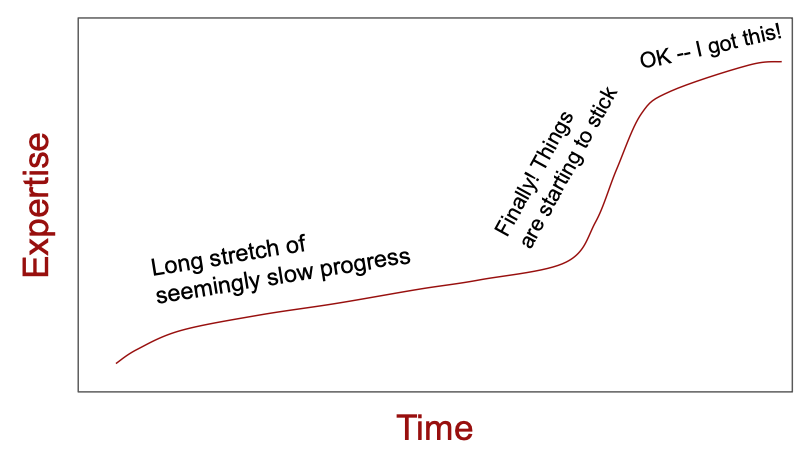
\includegraphics[width=11.21in]{images/01_001_r_learning_curve_past} 

}

\caption{\label{fig:1001}R learning curve past}\label{fig:1001}
\end{figure}

The R programming language is still challenging but worth it. With the introduction of packages encompassed in the tidyverse there are more high-quality resources, mature utilization with well documented explanations and examples. Currently there is lots of current interest in R with a large community of users and developers. Additionally, the data science ``revolution has pushed R to develop and evolve, become more user-centric.

\begin{figure}

{\centering 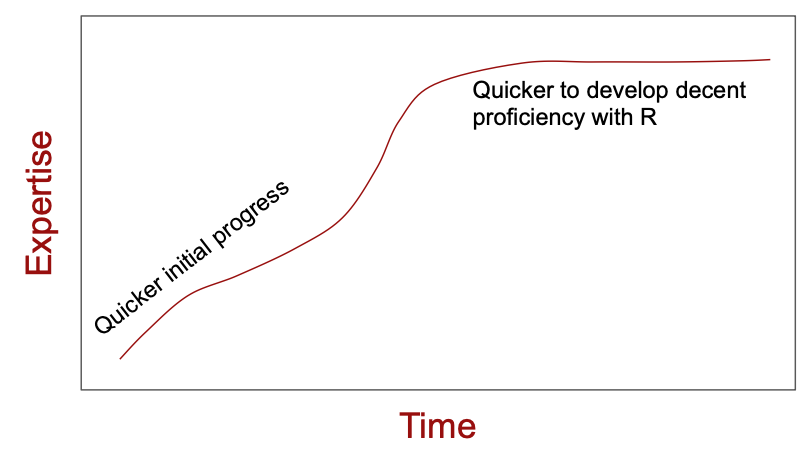
\includegraphics[width=11.21in]{images/01_002_r_learning_curve_present} 

}

\caption{\label{fig:1002}R learning curve present}\label{fig:1002}
\end{figure}

\hypertarget{thoughts-about-learning-r-and-how-to-code}{%
\section*{Thoughts about learning R and how to code}\label{thoughts-about-learning-r-and-how-to-code}}
\addcontentsline{toc}{section}{Thoughts about learning R and how to code}

When it comes to learning a programming language, it can be daunting to know where to start. However, the first step to learning any programming language is to understand its syntax. Syntax refers to the set of rules and symbols that make up structurally correct code. Without proper syntax, even the smallest of errors can result in code that doesn't run. These errors could be as simple as a typo, an incorrect name, missing spaces or too many spaces, or even wrong brackets. Syntax errors can be frustrating, especially for beginners, but it's important to hang in there and start simple.

It's best to begin by trying to understand very simple cases first, before building and expanding on them. This approach will help you to get a better grip on the basics of the language and will help you to avoid becoming overwhelmed. If you're learning R, there are many resources available to help you get started. You could start by reading through the R Book, which provides a comprehensive guide to the R programming language. Alternatively, there are many online tutorials available, which can help to break down complex concepts into more manageable pieces.

In short, when learning R, it's important to remember that syntax is key. By taking the time to understand the syntax rules, you can avoid frustrating syntax errors and build a solid foundation for your future coding endeavors

\hypertarget{alternatives}{%
\section*{Alternatives}\label{alternatives}}
\addcontentsline{toc}{section}{Alternatives}

When it comes to data science, R is a popular programming language among statisticians and data analysts. However, there are several data science alternatives to R that are also gaining popularity.

One of the most popular alternatives to R is Python. Python is a general-purpose programming language that has a wide range of libraries and frameworks for data science. It is known for its simplicity, readability, and versatility. Python's libraries such as NumPy, Pandas, and Scikit-Learn are widely used in data science for tasks such as data cleaning, data analysis, and machine learning.

Another alternative to R is Julia, a new programming language that is designed specifically for scientific computing and numerical analysis. Julia is known for its speed and efficiency, making it a great choice for data analysis and modeling. Julia also has a growing package ecosystem with libraries such as DataFrames.jl and Flux.jl that are specifically designed for data science.

Matlab is another alternative to R that is widely used in the scientific community. Matlab is known for its extensive numerical computing capabilities and its strong visualization features. It is commonly used in fields such as engineering, physics, and finance for data analysis and modeling.

In conclusion, while R is a popular language for data science, it is not the only option available. Python, Julia, and Matlab are all viable alternatives with their own strengths and weaknesses. It is important to consider the specific needs of your project and choose the programming language that best suits your requirements.

\hypertarget{did-you-know}{%
\subsection*{Did you know}\label{did-you-know}}
\addcontentsline{toc}{subsection}{Did you know}

While R on its own is a powerful scripting language, some analytical tasks might require the use of other programming languages such as Python, C++ or Rust. Luckily, R provides different packages that allow us to use these languages within R code. These packages provide a seamless integration between these languages and R, allowing you to leverage the strengths of each language to perform complex tasks.

The \texttt{reticulate} package enables the integration of Python code in R. This package allows you to import Python modules and functions directly into R and also allows you to call Python functions from R code. This is especially useful when you need to use Python's machine learning libraries such as TensorFlow or PyTorch, which are not yet available in R.

Similarly, the \texttt{Rcpp} package provides a smooth integration between R and C++. With this package, you can easily write C++ functions and use them directly in your R code. This is useful when you need to perform computationally-intensive tasks, such as simulations or optimization, that require the speed of C++.

Finally, the \texttt{extendr} package provides an interface between R and Rust, allowing you to use Rust functions in R code and vice versa. Rust is a relatively new programming language that provides a balance between performance and safety. It is especially useful when you need to develop high-performance and low-level code, such as in systems programming or hardware development.

\hypertarget{installation}{%
\chapter{Installation}\label{installation}}

In the scope of this book, there are three main components that need to be installed, and periodically updated:

\begin{itemize}
\item
  \textbf{The R interpreter} - the software that understands math and plotting
\item
  \textbf{RStudio IDE} - the software that makes it easy write code and visualize data
\item
  \textbf{R Packages} - bits of R code that perform specalized operations
\end{itemize}

In this book we will be utilizing the RStudio integrated development environment (IDE) to interact with R. Two separate components are required for this - the R interpreter and the RStudio IDE. Both are required as the RStudio IDE only provides an interface for the R interpreter, which reads the code and does all the mathematical operations. The R interpreter can be used alone, interacting through the command line (eg. Windows CMD, MacOS and Linux Terminal), a plain text editor or another IDE such as Xcode, VSCode, Eclipse, Notepad++, etc. Rstudio provides a comprehensive, R specific environment, with auto-complete, code syntax highlighting, in-editor function definitions along with package management and plot visualizations.

\begin{infobox}{skill}
At the end of this chapter you should be able to:\\
1. Install R, RStudio and a few R packages\\
2. Understand the major components for working with R.

\end{infobox}

\hypertarget{r-interpreter}{%
\section{R interpreter}\label{r-interpreter}}

The underlying ``engine'' for R programming language can be downloaded from \href{https://www.r-project.org/}{The R Project for Statistical Computing}. R is an open-source implementation of the S statistical computing language originally developed at Bell Laboratories. Both langauges contain a variety of statistical and graphical techniques, however, R has been continually extended by professional, academic and amateur contributors and remains the most active today. With the advent of open-source sharing platforms such as GitHub, R has become increasingly popular among data scientists because of its ease of use and flexibility in handling complex analyses on large datasets. Additionally, one of R's strengths is the ease with which well-designed publication-quality plots can be produced.

\hypertarget{steps}{%
\subsubsection*{Steps}\label{steps}}
\addcontentsline{toc}{subsubsection}{Steps}

\begin{enumerate}
\def\labelenumi{\arabic{enumi}.}
\tightlist
\item
  Navigate to \href{https://www.r-project.org/}{The R Project}
\item
  Click on \href{https://cran.r-project.org/mirrors.html}{CRAN} under Download, left-hand side
\item
  Click on \url{https://cloud.r-project.org/} under 0-Cloud\\
  \emph{This will take you to the globally nearest up-to-date repository}
\item
  Click on \texttt{Download\ for\ ...} and choose the OS compatible with your device
\end{enumerate}

\hypertarget{windows-os}{%
\subsubsection*{Windows OS}\label{windows-os}}
\addcontentsline{toc}{subsubsection}{Windows OS}

Click on \texttt{base}

\hypertarget{macos}{%
\subsubsection*{MacOS}\label{macos}}
\addcontentsline{toc}{subsubsection}{MacOS}

\textbf{For an Intel CPU}: click \texttt{R-4.x.x.pgk} to download\\
\textbf{For an M1 CPU}: click \texttt{R-4.x.x-arm64.pkg} to download

After downloading, double-click the installer and follow the instructions

\begin{figure}
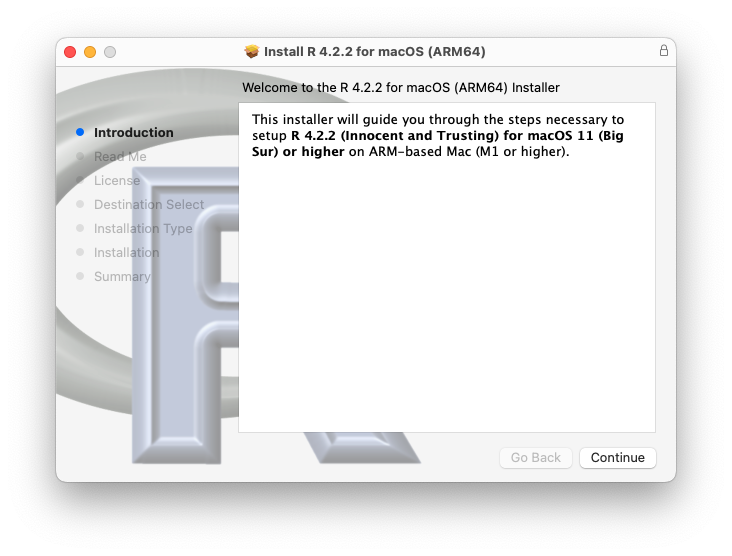
\includegraphics[width=10.17in]{images/02_001_r_installer_mac_m1} \caption{\label{fig:2001}Mac Installer}\label{fig:2001}
\end{figure}

\hypertarget{linux}{%
\subsubsection*{Linux}\label{linux}}
\addcontentsline{toc}{subsubsection}{Linux}

Click on your distribution and follow the instructions provided. Most of these instructions require knowledge of the Terminal and command line interface for *unix systems.

\hypertarget{rstudio}{%
\section{Rstudio}\label{rstudio}}

RStudio, prior to 2023, was an independent software provider for the ever-popular RStudio products, which included both the desktop and server based IDEs, along with the RShiny applications and servers that facilitate easy-to-build interactive web applications straight from R, and deployed on the web. The last chapter in this book will explore the \texttt{tidyproteomics} package which also has a Shiny web application. RStudio announced at the beginning of 2023 a soft pivot to Posit, which essentially is a rebranding of the RStudio company to encompass a larger data science audience, one that also provides integration with the Python programming language inside the RStudio IDE.

\begin{quote}
The most trusted IDE for open source data science

``RStudio is an integrated development environment (IDE) for R and Python. It includes a console, syntax-highlighting editor that supports direct code execution, and tools for plotting, history, debugging, and workspace management. RStudio is available in open source and commercial editions and runs on the desktop (Windows, Mac, and Linux).''

--- www.posit.co (Jan 2023)
\end{quote}

\hypertarget{steps-1}{%
\subsubsection*{Steps}\label{steps-1}}
\addcontentsline{toc}{subsubsection}{Steps}

\begin{enumerate}
\def\labelenumi{\arabic{enumi}.}
\tightlist
\item
  Navigate to \href{https://posit.co/}{posit.co}, alternatively \href{https://rstudio.com/}{rstudio.com} redirects to the Posit website.
\item
  \textbf{Click} \texttt{Download\ RStudio} in the menu top right
\item
  Select \texttt{RStudio\ Desktop}
\item
  \textbf{Click} \texttt{Download\ RStudio}\\
  \emph{skip 1: Install R}
\item
  \textbf{Click} \texttt{Download\ RStudio\ Desktop\ for\ ..}
\end{enumerate}

\hypertarget{windows-os-1}{%
\paragraph*{Windows OS}\label{windows-os-1}}
\addcontentsline{toc}{paragraph}{Windows OS}

\hypertarget{macos-1}{%
\paragraph*{MacOS}\label{macos-1}}
\addcontentsline{toc}{paragraph}{MacOS}

Opening the .dmg file shows the archive that can be copied into the Applications folder simply by click-dragging the application onto the Applications folder shortcut.

\begin{figure}
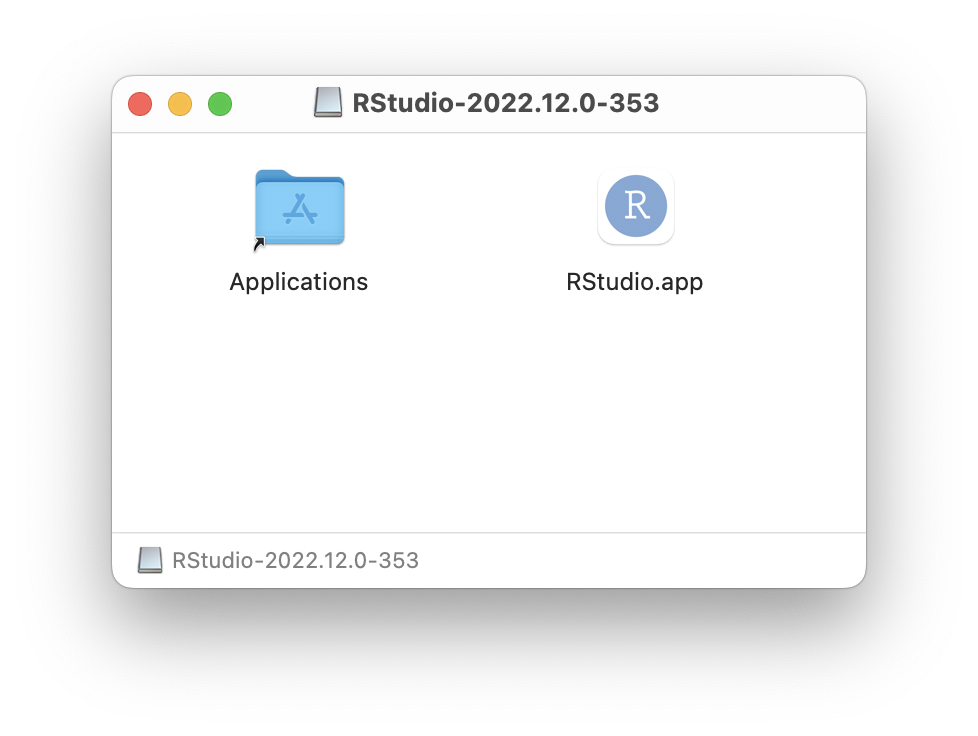
\includegraphics[width=13.58in]{images/02_011_rstudio_installer_mac} \caption{\label{fig:2011}RStudio IDE Install}\label{fig:2011}
\end{figure}

\hypertarget{linux-1}{%
\paragraph*{Linux}\label{linux-1}}
\addcontentsline{toc}{paragraph}{Linux}

\hypertarget{ide-layout}{%
\subsection{IDE Layout}\label{ide-layout}}

The RStudio Integrated Development Environment (IDE) is a powerful tool that can make your data analysis and coding tasks more manageable. One of the key features of the RStudio IDE is that it consists of four individual panes, each containing parts of the total environment. This makes it easier for you to navigate your coding and analysis tasks.

For example, while creating and viewing a plot, you can have the text editor and console open and organized. This way, you can easily see how the code you are writing is impacting the plot you are creating. Having everything in one place can also help reduce the clutter on your desktop, as you don't need to have multiple applications open at the same time.

Overall, the RStudio IDE is an excellent option for anyone looking to streamline their coding and data analysis workflows. By taking advantage of its various features, you can make your work more efficient and enjoyable.

\begin{figure}
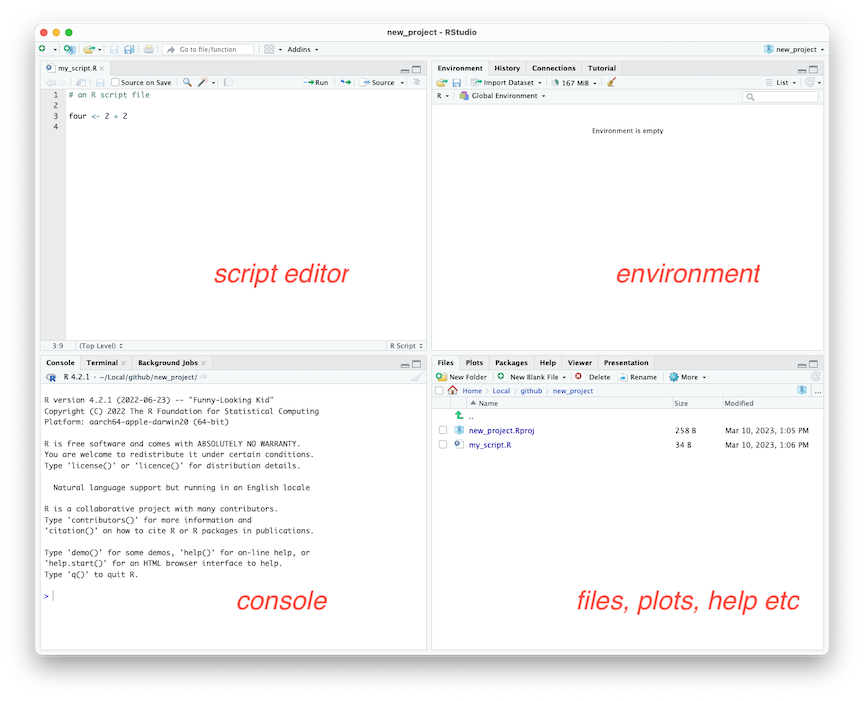
\includegraphics[width=19.19in]{images/02_021_rstudio_panes} \caption{\label{fig:2021}RStudio IDE in the default layout}\label{fig:2021}
\end{figure}

\hypertarget{the-editor}{%
\subsubsection*{The Editor}\label{the-editor}}
\addcontentsline{toc}{subsubsection}{The Editor}

\begin{quote}
\textbf{Tabs}: \texttt{All\ Open\ Files}
\end{quote}

The \emph{Editor} is a tool that allows you to write R code with ease. It is essentially a text editor, but with the added benefit of having knowledge of R. This means that it can automatically color different parts of your code based on their function. This can be a huge time saver, as it makes it easier to read and understand your code.

For example, comments in R code start with a hash (\#) symbol. In the \emph{Editor}, these comments are colored light green, making them easy to spot. Similarly, operators like the plus sign (+) and the assignment operator (\textless-) are colored light blue. This makes it easy to identify where these operators are being used in your code.

Variables are an important part of any programming language, and R is no exception. In the \emph{Editor}, variables are colored black. This makes it easy to distinguish variable names from other parts of your code. Finally, quoted text (also known as strings) are colored purple. This makes it easy to identify where strings are being used in your code.

In summary, the \emph{Editor} is a powerful tool that can help you write R code more efficiently. By automatically coloring different parts of your code, it makes it easier to read and understand. Whether you are a beginner or an experienced R programmer, the \emph{Editor} can help you write better code in less time.

\begin{figure}
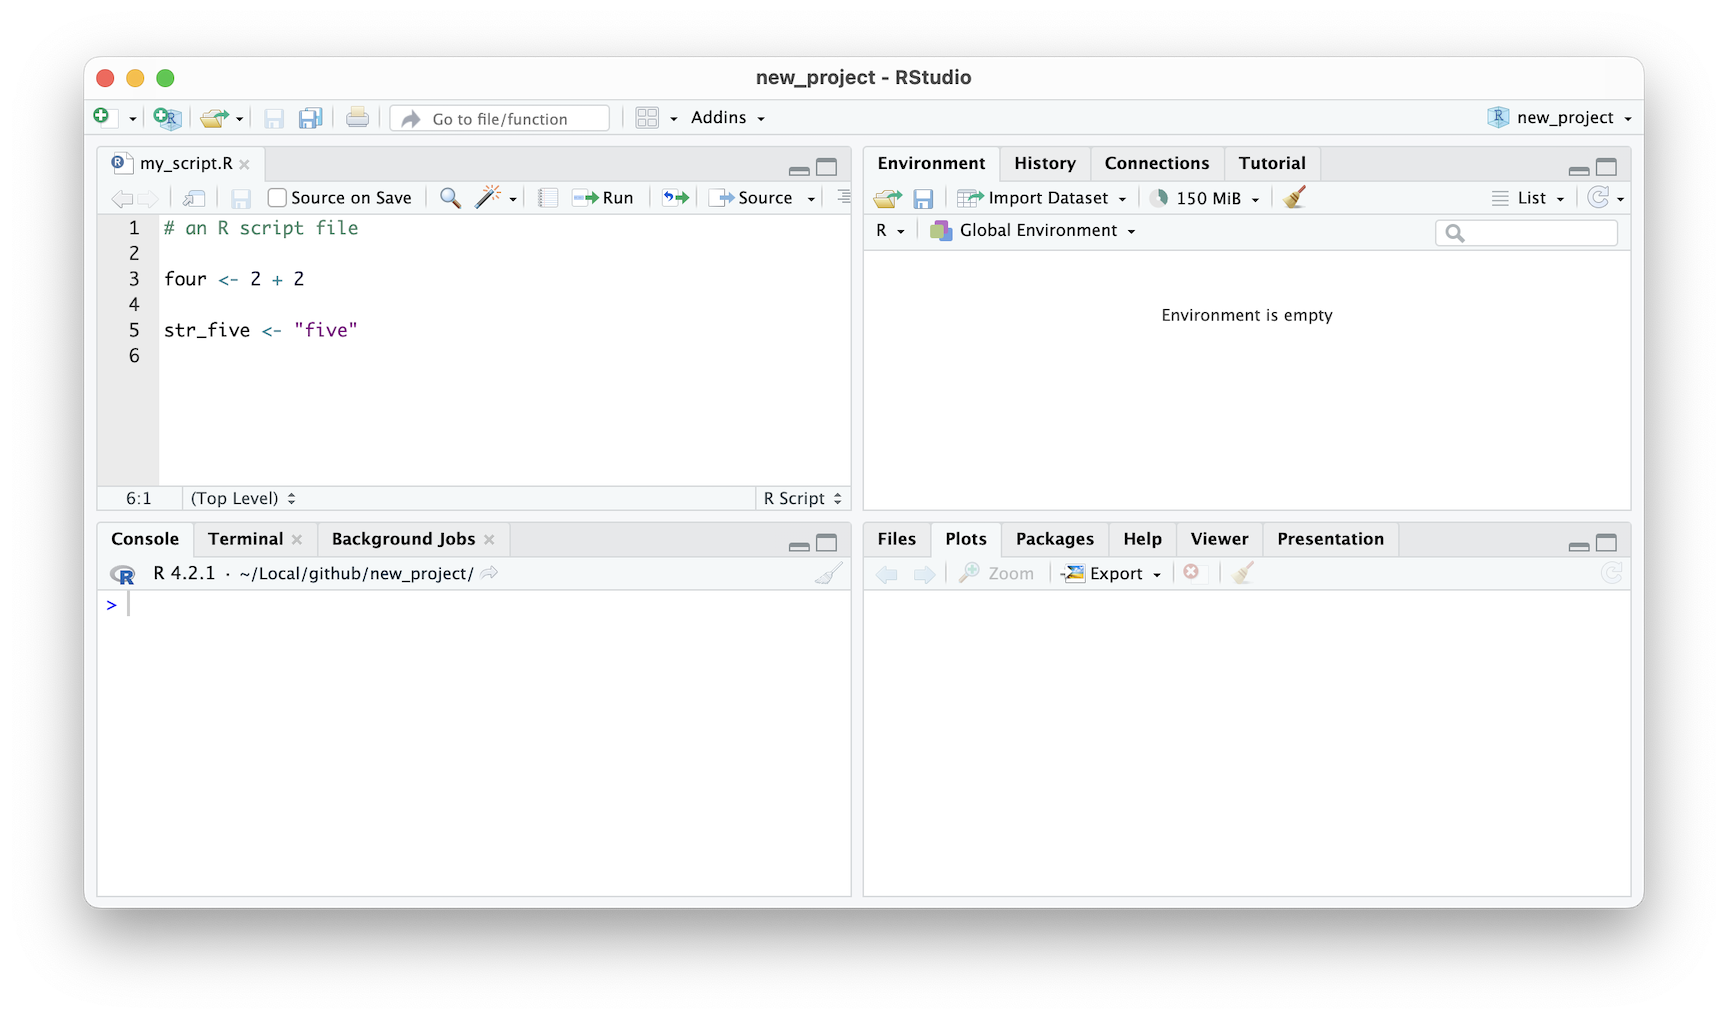
\includegraphics[width=31.94in]{images/02_022_editor_highlighting} \caption{\label{fig:2022}RStudio IDE syntax highlighting}\label{fig:2022}
\end{figure}

The Editor also has the ability to suggest available variables and functions. In the image provided, the editor suggests using the mean() function to calculate the average of a collection of values. A pop-up with a description accompanies the suggestion. This feature occurs after typing in the first three letters of anything, and the editor will try to guess what you want to type next. This is a helpful tool that can save you time and effort when writing R code.

\begin{figure}
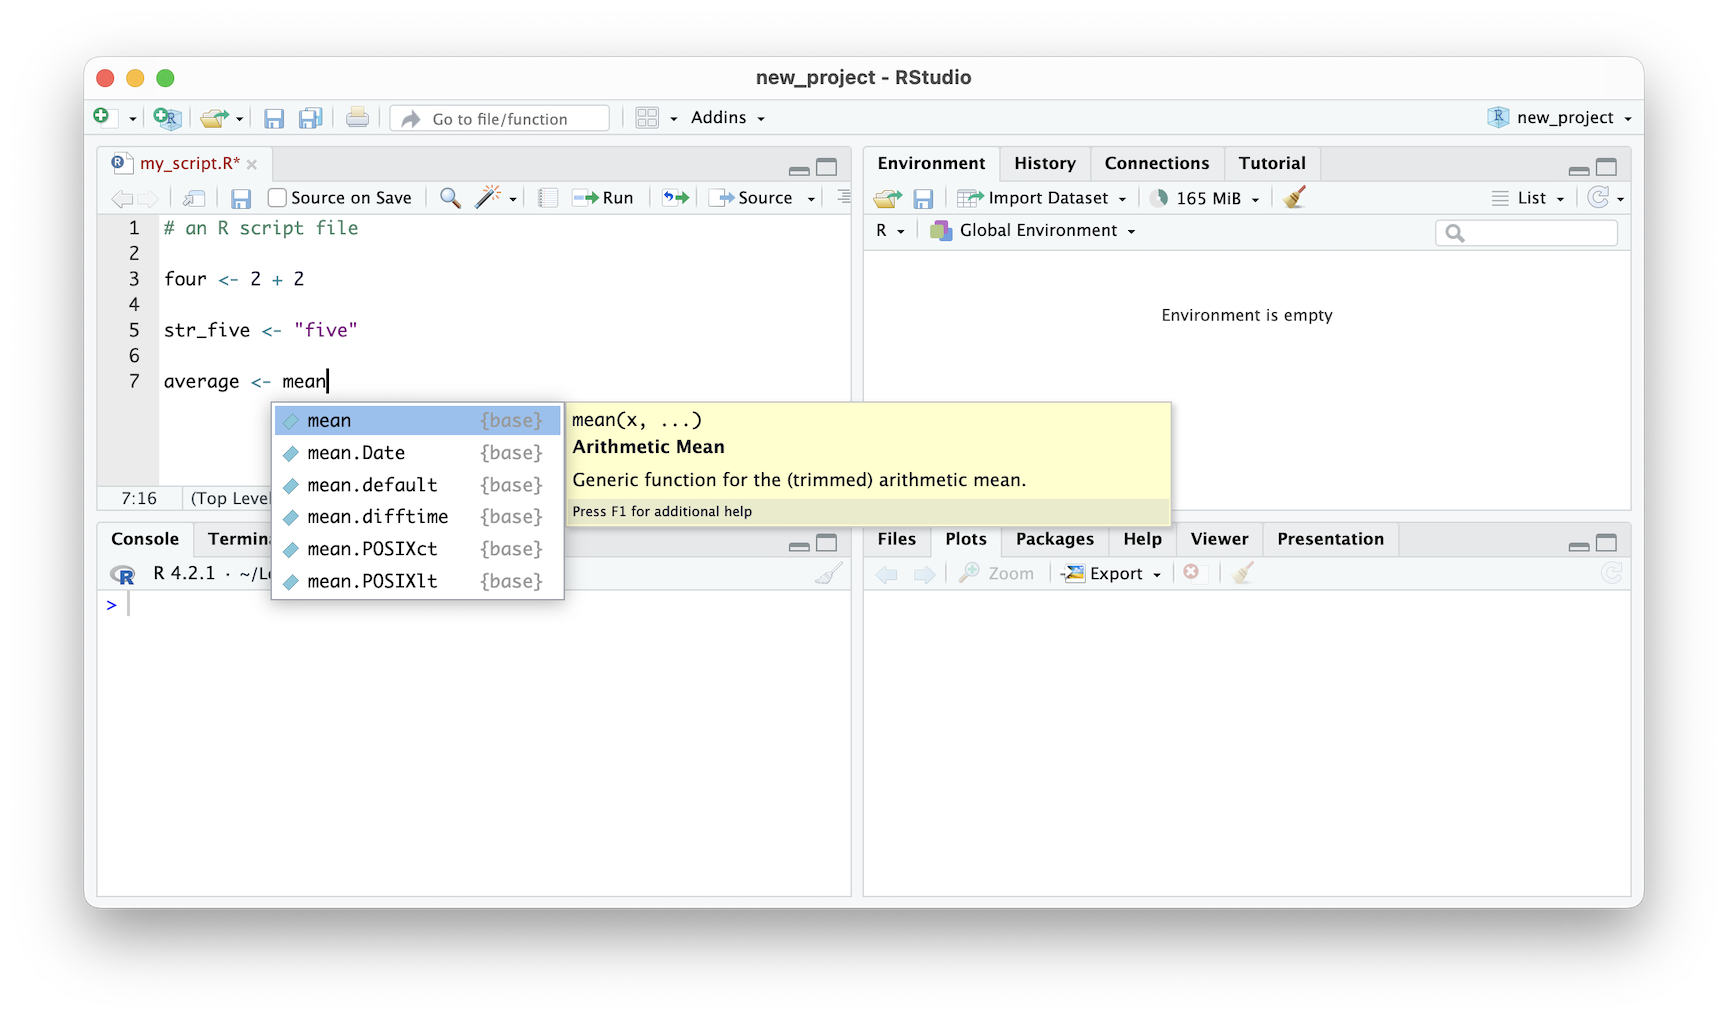
\includegraphics[width=31.94in]{images/02_023_editor_autocomplete} \caption{\label{fig:2023}RStudio IDE auto complete}\label{fig:2023}
\end{figure}

\hypertarget{files-and-plots}{%
\subsubsection*{Files and Plots}\label{files-and-plots}}
\addcontentsline{toc}{subsubsection}{Files and Plots}

\begin{quote}
\textbf{Tabs}: \texttt{Files}, \texttt{Plots}, \texttt{Packages}, \texttt{Viewer}, and \texttt{Presentation}
\end{quote}

When you're working in RStudio, your workflow is made simple with the various tabs and features available. For instance, the script that you're currently working on is saved to the current project and can be accessed via the \emph{Files} tab located on the top right-hand side of the pane. This tab provides an overview of all the files in the working directory, and you can easily navigate between them.

If you need to open another file, you can do so by clicking on the \emph{File} menu or by using the shortcut key. When you open a new file, it will create a new tab in the \emph{Editor} pane, which allows you to switch between open files. This feature is super helpful when you're working on multiple files simultaneously.

Another useful tab located in the same pane is the \emph{Plots} tab. This tab provides a quick way to view any active plots instantly. You don't need to export your plots or save them separately. Instead, you can view them right within RStudio. This is where RStudio truly shines, as it brings together editing and visualization in one application.

\begin{figure}
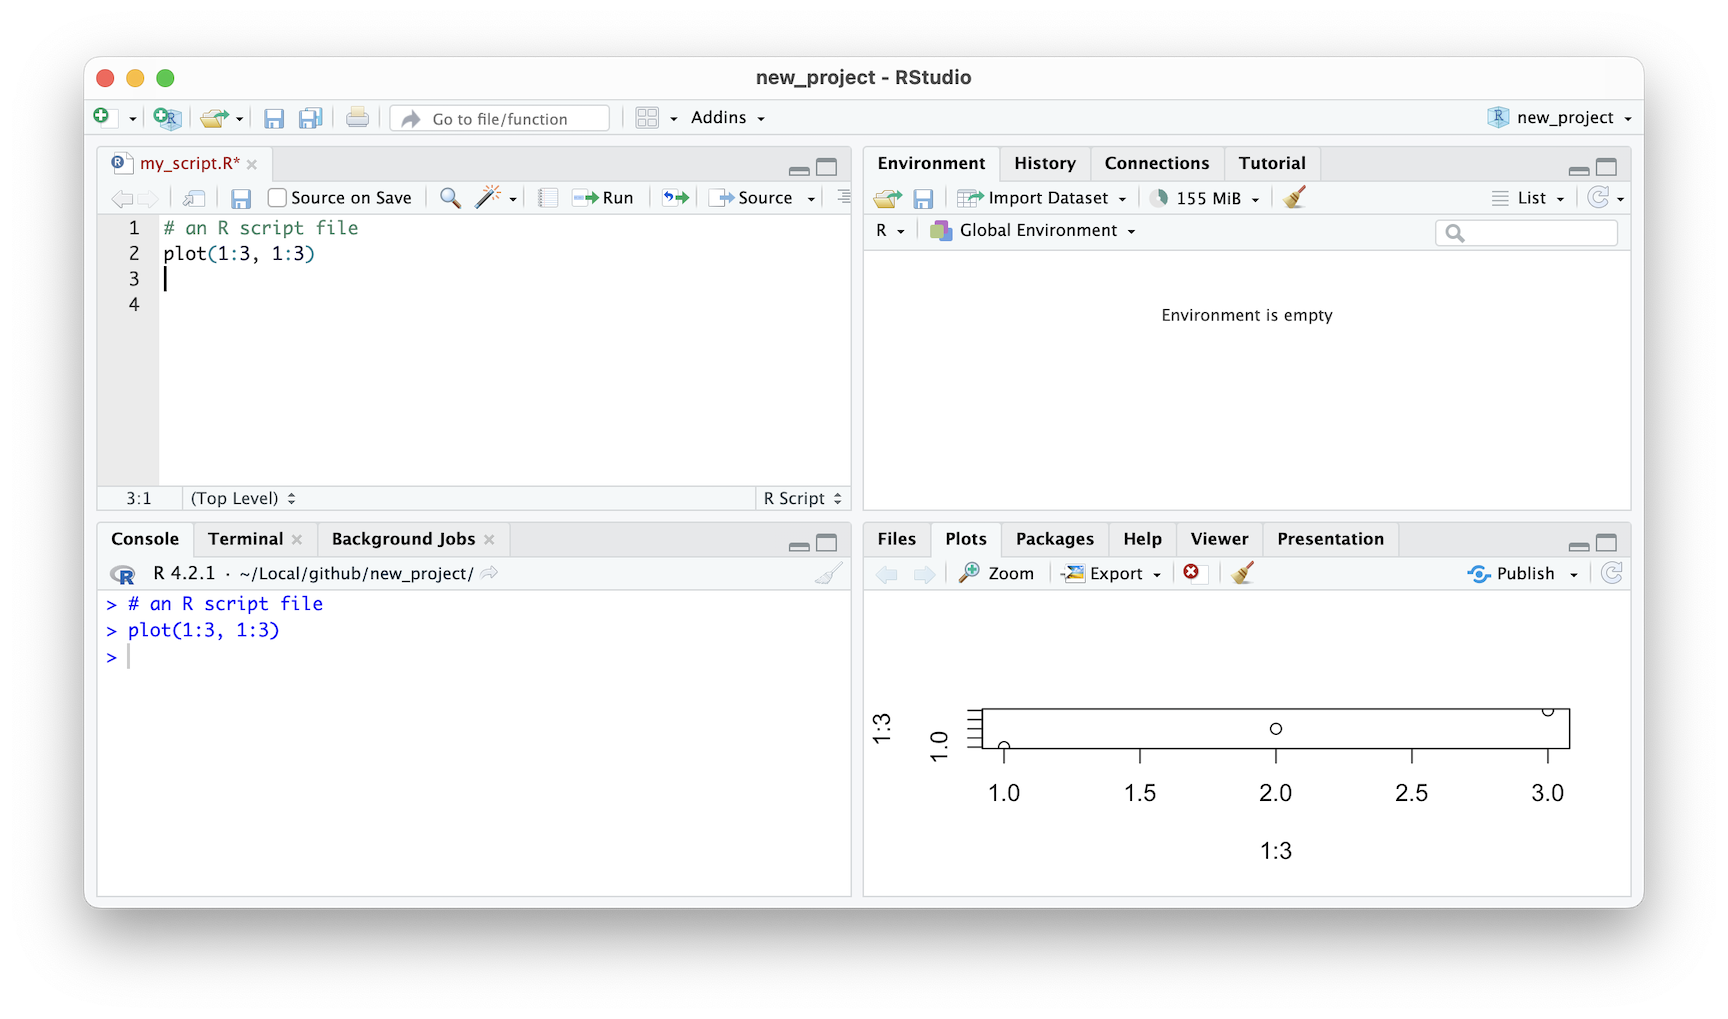
\includegraphics[width=31.94in]{images/02_024_qplot} \caption{\label{fig:2024}RStudio IDE plot window}\label{fig:2024}
\end{figure}

\hypertarget{the-console}{%
\subsubsection*{The Console}\label{the-console}}
\addcontentsline{toc}{subsubsection}{The Console}

\begin{quote}
\textbf{Tabs}: \texttt{Console}, \texttt{Terminal}, and \texttt{Background\ Jobs}
\end{quote}

In the RStudio IDE, the \emph{Console} pane is where lines of code are executed from the editor. It is a vital component of the RStudio interface that allows users to interact with R in real-time. The \emph{Console} pane is not only where code is run, but it is also where users can view output and error messages. Additionally, the \emph{Console} pane provides users access to the computer's terminal. This feature allows users to execute commands outside of the R environment, such as navigating files and directories or installing packages. Overall, the \emph{Console} pane is an essential tool for any RStudio user and should be utilized to its full potential.

\hypertarget{environment}{%
\subsubsection*{Environment}\label{environment}}
\addcontentsline{toc}{subsubsection}{Environment}

\begin{quote}
\textbf{Tabs}: \texttt{Environment}, \texttt{History}, \texttt{Connections}, and \texttt{Tutorial}
\end{quote}

When you're working on a project in R, it's essential to keep track of the variables and functions that you're using in your current session. The \emph{Environment} tab, located at the top left of the RStudio interface, provides a concise summary of in-memory variables and functions that were created locally, as opposed to functions that were loaded from a package.

This summary can be useful for new-comers to R because it allows you to quickly see what objects you are currently working with, without having to remember each or manually check. By having a clear overview of your current session, you can avoid mistakes or errors that might arise from using the wrong object or function.

Overall, the \emph{Environment} tab is a helpful feature of RStudio that can save you time and frustration. If you're new to R or just starting to use RStudio, make sure to keep an eye on the \emph{Environment} tab and make use of its features as often as possible. As you become more versed in RStudio this tab may become less relevant.

\begin{figure}
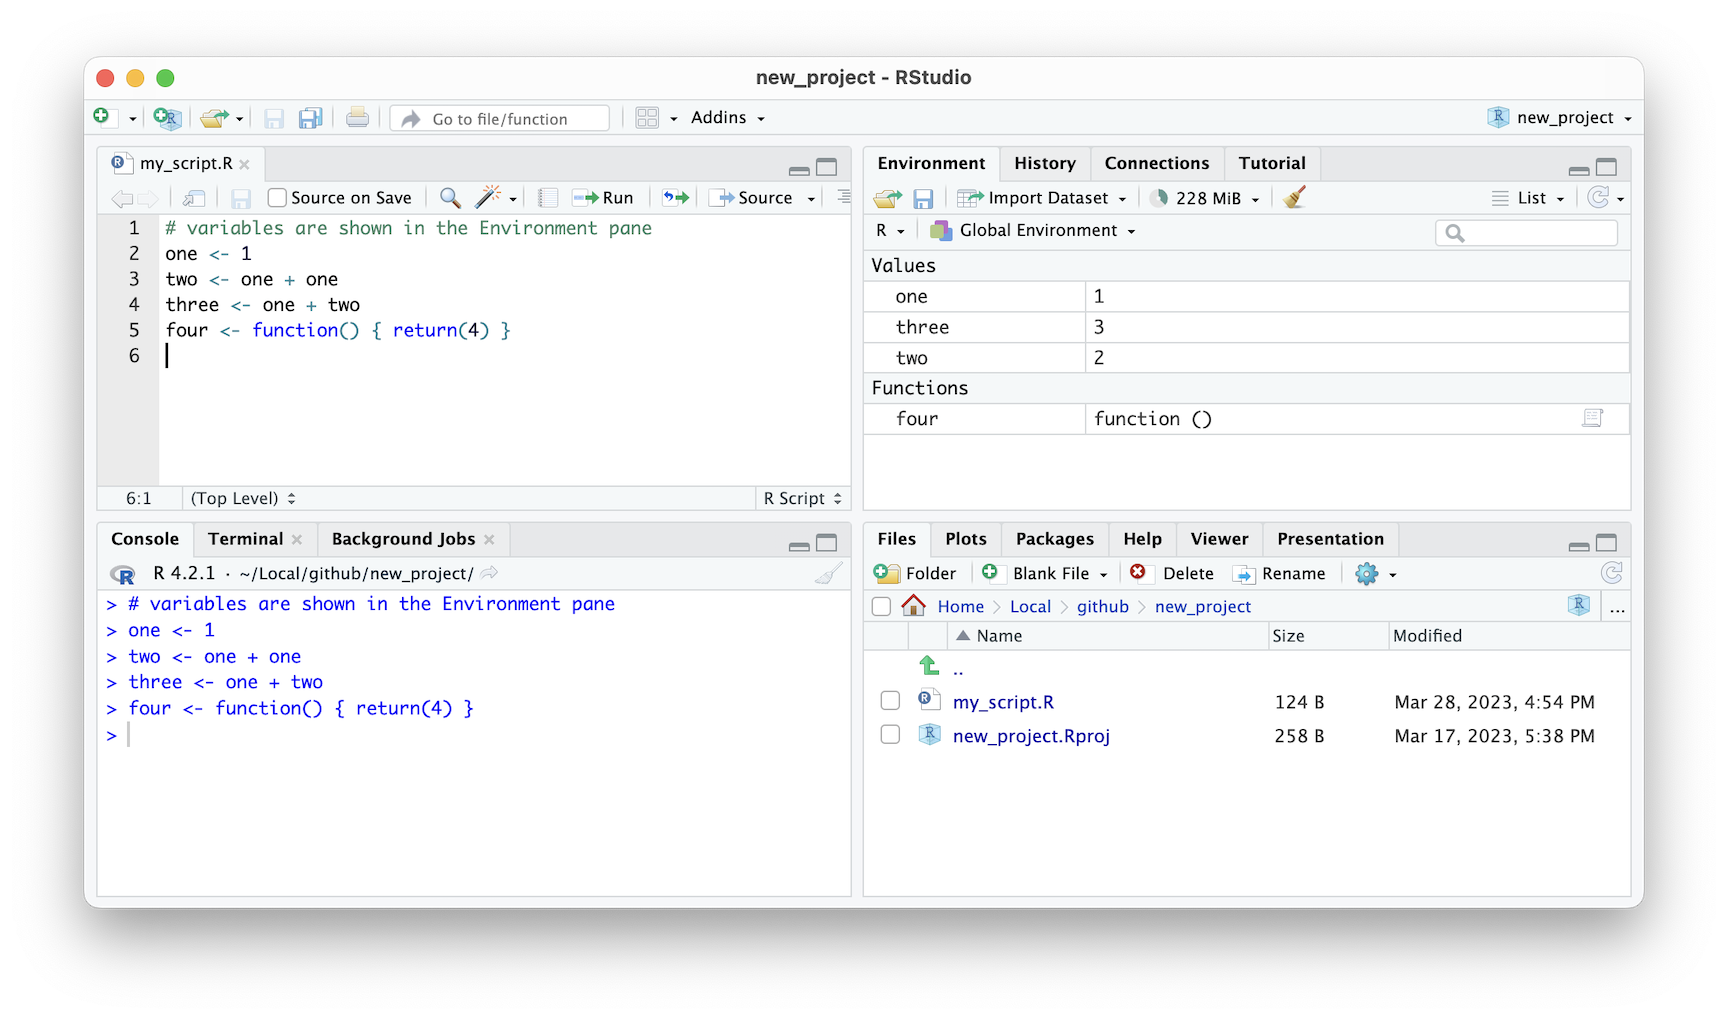
\includegraphics[width=31.94in]{images/02_025_environment} \caption{\label{fig:2025}RStudio IDE environment window}\label{fig:2025}
\end{figure}

\hypertarget{usage-..-running-lines-of-code-in-rstudio}{%
\subsection{Usage .. Running lines of code in RStudio}\label{usage-..-running-lines-of-code-in-rstudio}}

\hypertarget{run-from-the-editor-recommended}{%
\subsubsection{Run from the editor (recommended)}\label{run-from-the-editor-recommended}}

\begin{enumerate}
\def\labelenumi{\arabic{enumi}.}
\tightlist
\item
  Type in the code in the Editor (top-left pane)
\item
  Put editor cursor anywhere on that line
\item
  Press Ctrl/CMD+Enter.
\item
  Multiple lines: highlight multiple lines then press Ctrl/CMD+Enter \#\#\#\# Run from the onsole (occasionally)
\item
  Type code into Console (bottom-left) after the `\textgreater{}'
\item
  Press Enter.
\item
  Multiple lines, not advised, but copy and paste multiple lines into console then press Enter.
\end{enumerate}

\hypertarget{packages}{%
\section{Packages}\label{packages}}

\hypertarget{what-are-r-packages}{%
\subsection{What are R Packages?}\label{what-are-r-packages}}

R packages are a powerful tool in the R programming language that allow you to easily use code written by others in your own projects. They can save a lot of time and effort in the development of your own code, as they often provide new functions to deal with specific problems. For example, the popular ggplot2 package provides a variety of functions to help you create beautiful visualizations, while the mzR package allows you to read mass spectrometry data files with ease. Additionally, the twitteR package is a great tool for accessing Twitter data and conducting analysis.

\hypertarget{where-to-get-r-packages}{%
\subsection{Where to get R Packages}\label{where-to-get-r-packages}}

It's worth noting that packages can be written by anyone, which means that their quality can vary widely. While there are many high-quality packages available, it's important to be wary of randomly coming across packages on the internet. To ensure that you're working with trustworthy code, it's a good idea to stick with well-established and frequently updated packages from reputable sources such as the CRAN (The Comprehensive R Archive Network) and Bioconductor repositories. By doing so, you can ensure that your code is reliable, efficient, and secure.

\begin{itemize}
\tightlist
\item
  CRAN \href{https://cran.r-project.org/}{cran.r-project.org}
\item
  Bioconductor \href{https://bioconductor.org/}{bioconductor.org}
\item
  GitHub \href{https://github.com/}{github.com}
\end{itemize}

In addition to using established packages, it's also possible to create your own packages in R. This is a great way to share your own code with others and make it accessible to a wider audience. When creating a package, it's important to follow a set of best practices to ensure that your code is well-documented, easy to use, and compatible with other packages. This includes providing clear and concise documentation, including examples and tutorials, and following established coding conventions.

Another important consideration when working with R packages is version control. It's essential to keep track of the versions of the packages you're using, as updates can sometimes break existing code. By using a tool like Git or GitHub, you can easily manage different versions of your code and keep track of changes over time. This can be especially useful when collaborating with others on a project.

Overall, R packages are an essential tool for anyone working with R. By using established packages and following best practices when creating your own, you can ensure that your code is efficient, reliable, and easy to use. And by using version control, you can keep track of changes over time and collaborate effectively with others.

\hypertarget{installing-r-packages}{%
\subsection{Installing R Packages}\label{installing-r-packages}}

When working with R, it is important to understand how to install packages. R packages are collections of functions, data, and documentation that extend the capabilities of R. Most R packages have binary versions available for direct installation with no additional steps required. Binary packages are pre-compiled and ready-to-use packages that are platform-specific. They can be installed with the \texttt{install.packages()} function in R.

\begin{infobox}{note}
Follow the examples below to install all the required packages used in this book. Jump to the following section if you run into any issues. Use the copy-paste button in the top-right of each code block.

\end{infobox}

\hypertarget{installing-from-cran}{%
\subsubsection*{Installing from CRAN}\label{installing-from-cran}}
\addcontentsline{toc}{subsubsection}{Installing from CRAN}

\begin{Shaded}
\begin{Highlighting}[]
\CommentTok{\# this installs all of the packages in the tidyverse collection}
\FunctionTok{install.packages}\NormalTok{(}\StringTok{\textquotesingle{}tidyverse\textquotesingle{}}\NormalTok{)}
\end{Highlighting}
\end{Shaded}

\hypertarget{installing-from-bioconductor}{%
\subsubsection*{Installing from Bioconductor}\label{installing-from-bioconductor}}
\addcontentsline{toc}{subsubsection}{Installing from Bioconductor}

\begin{Shaded}
\begin{Highlighting}[]
\CommentTok{\# do this once to install the Bioconductor Package Manager}
\FunctionTok{install.packages}\NormalTok{(}\StringTok{"BiocManager"}\NormalTok{)}
\CommentTok{\# this installs the mzR package}
\NormalTok{BiocManager}\SpecialCharTok{::}\FunctionTok{install}\NormalTok{(}\FunctionTok{c}\NormalTok{(}\StringTok{"mzR"}\NormalTok{, }\StringTok{"xcms"}\NormalTok{, }\StringTok{"MSstats"}\NormalTok{, }\StringTok{"MSnbase"}\NormalTok{))}
\end{Highlighting}
\end{Shaded}

\hypertarget{installing-from-github}{%
\subsubsection*{Installing from GitHub}\label{installing-from-github}}
\addcontentsline{toc}{subsubsection}{Installing from GitHub}

\begin{Shaded}
\begin{Highlighting}[]
\CommentTok{\# do this once to install the devtools package }
\FunctionTok{install.packages}\NormalTok{(}\StringTok{"devtools"}\NormalTok{)}
\CommentTok{\# this installs the tidyproteomics package}
\FunctionTok{install\_github}\NormalTok{(}\StringTok{"jeffsocal/tidyproteomics"}\NormalTok{)}
\end{Highlighting}
\end{Shaded}

\begin{infobox}{note}
There maybe several additional packages to install including additional operating system level installs. Go to the \href{https://jeffsocal.github.io/tidyproteomics/}{tidyproteomics} webpage for additional installation help.

\end{infobox}

\hypertarget{potential-gotchas}{%
\subsection{Potential Gotchas}\label{potential-gotchas}}

However, there are cases where a binary version of a package may not be available. This could be because the package is new or has just been updated. In such cases, the package may need to be compiled before it can be installed. Compiling a package involves converting the source code into machine-readable code that can be executed.

To compile R packages, you'll need to have the necessary programs and libraries installed on your computer. For Windows, you'll need to install RTools, which provides the necessary tools for package compilation. For Mac, you'll need to install Command Line Tools. Once these tools are installed, you can use them to compile packages that are not available as binaries.

However, it's worth noting that package compilation can sometimes fail for various reasons. This can be frustrating, especially if you're new to R. Therefore, it is generally recommended to stick with using binary packages whenever possible. Binary packages are more stable and easier to install, making them the preferred option for most users.

In summary, when working with R, it's important to understand how to install packages. Most packages have binary versions available for direct installation, but there may be cases where you need to compile a package yourself. While package compilation can be useful in some cases, it can also be frustrating and time-consuming. Therefore, it's generally recommended to stick with using binary packages whenever possible.

\hypertarget{packages-utilized-in-this-book}{%
\section{Packages Utilized in This Book}\label{packages-utilized-in-this-book}}

\hypertarget{tidyverse}{%
\subsection{tidyverse}\label{tidyverse}}

The Tidyverse R package is a collection of data manipulation and visualization packages for the R programming language. It includes popular packages such as dplyr, ggplot2, and tidyr, among others. The Tidyverse R package is a powerful and versatile tool for data analysis in R. It includes a collection of data manipulation and visualization packages designed to work seamlessly together, making it easy to analyze and visualize data in R.

\begin{Shaded}
\begin{Highlighting}[]
\FunctionTok{library}\NormalTok{(tidyverse)}
\end{Highlighting}
\end{Shaded}

The \textbf{readr} package provides a versatile means of reading data from various formats, such as comma-separated (CSV) and tab-separated (TSV) delimitated flat files. In addition to its versatility, the \textbf{readr} package is also known for its speed and efficiency. It is designed to be faster than the base R functions for reading in data, making it an ideal choice for working with large datasets.

\begin{Shaded}
\begin{Highlighting}[]
\NormalTok{tbl }\OtherTok{\textless{}{-}} \StringTok{"./data/table\_peptide\_fragmnets.csv"} \SpecialCharTok{\%\textgreater{}\%} \FunctionTok{read\_csv}\NormalTok{()}
\end{Highlighting}
\end{Shaded}

\begin{verbatim}
## Rows: 14 Columns: 7
## -- Column specification -----------------------------------------------------------------------------------------------
## Delimiter: ","
## chr (4): ion, seq, pair, type
## dbl (3): mz, z, pos
## 
## i Use `spec()` to retrieve the full column specification for this data.
## i Specify the column types or set `show_col_types = FALSE` to quiet this message.
\end{verbatim}

The \textbf{tibble} package embodies a modern, flexible take on the data table, making it a powerful tool for data analysis in R. This package includes a suite of functions that allow you to easily manipulate and reshape data. It also has a printing method that makes it easy to view and explore data, even when dealing with large datasets. Additionally, tibble objects are designed to work seamlessly with other Tidyverse packages, such as \textbf{dplyr} and \textbf{tidyr}, making it easy to switch between packages and maintain a consistent syntax.

\begin{Shaded}
\begin{Highlighting}[]
\FunctionTok{print}\NormalTok{(tbl)}
\end{Highlighting}
\end{Shaded}

\begin{verbatim}
## # A tibble: 14 x 7
##    ion      mz     z seq     pair    pos type     
##    <chr> <dbl> <dbl> <chr>   <chr> <dbl> <chr>    
##  1 b1+    98.1     1 P       p01       1 b        
##  2 y1+   148.      1 E       p06       1 y        
##  3 b2+   227.      1 PE      p02       2 b        
##  4 y2+   263.      1 DE      p05       2 y        
##  5 b3+   324.      1 PEP     p03       3 b        
##  6 y3+   376.      1 IDE     p04       3 y        
##  7 MH++  401.      2 PEPTIDE p00      NA precursor
##  8 b4+   425.      1 PEPT    p04       4 b        
##  9 y4+   477.      1 TIDE    p03       4 y        
## 10 b5+   538.      1 PEPTI   p05       5 b        
## 11 y5+   574.      1 PTIDE   p02       5 y        
## 12 b6+   653.      1 PEPTID  p06       6 b        
## 13 y6+   703.      1 EPTIDE  p01       6 y        
## 14 MH+   800.      1 PEPTIDE p00      NA precursor
\end{verbatim}

The \textbf{readxl} package is a complement to \textbf{readr} providing a means to read Excel files, both legacy .xls and the current xml-based .xlsx. It is capable of reading many different types of data, including dates, times, and various numeric formats. The package also provides options for specifying sheet names, selecting specific columns and rows, and handling missing values.

The \textbf{dplyr} package is widely known and used among data scientists and analysts for its interface that allows for easy and efficient data manipulation in \emph{tibbles}. Providing a set of ``verbs'' that are designed to solve common tasks in data transformations and summaries, such as filtering, arranging, and summarizing data, all designed to work seamlessly with other Tidyverse packages making it easy to switch between packages and maintain a consistent syntax. One of the key benefits of the \textbf{dplyr} package is its ease of use, making it perfect for beginners and advanced users alike. It is widely used in the R community and is a valuable tool for anyone working with R and data tables.

\begin{Shaded}
\begin{Highlighting}[]
\NormalTok{tbl }\SpecialCharTok{\%\textgreater{}\%} 
  \FunctionTok{filter}\NormalTok{(type }\SpecialCharTok{!=} \StringTok{\textquotesingle{}precursor\textquotesingle{}}\NormalTok{) }\SpecialCharTok{\%\textgreater{}\%} 
  \FunctionTok{group\_by}\NormalTok{(type) }\SpecialCharTok{\%\textgreater{}\%}
  \FunctionTok{summarise}\NormalTok{(}
    \AttributeTok{num\_ions =} \FunctionTok{n}\NormalTok{(),}
    \AttributeTok{avg\_mass =} \FunctionTok{mean}\NormalTok{(mz)}
\NormalTok{  )}
\end{Highlighting}
\end{Shaded}

\begin{verbatim}
## # A tibble: 2 x 3
##   type  num_ions avg_mass
##   <chr>    <int>    <dbl>
## 1 b            6     378.
## 2 y            6     424.
\end{verbatim}

The \textbf{tidyr} package contains a set of data table transformations, including pivotting rows to columns, splitting a single column into multiple ones, and tidying or cleaning up data tables for a more usable structure. These transformations are essential for dealing with real-world data tables, which are often messy and irregular. By using \textbf{tidyr}, you can quickly and easily manipulate data tables to extract the information you need and prepare them for further analysis.

\begin{Shaded}
\begin{Highlighting}[]
\NormalTok{tbl }\SpecialCharTok{\%\textgreater{}\%} 
  \FunctionTok{filter}\NormalTok{(type }\SpecialCharTok{==} \StringTok{\textquotesingle{}precursor\textquotesingle{}}\NormalTok{) }\SpecialCharTok{\%\textgreater{}\%} 
  \FunctionTok{pivot\_wider}\NormalTok{(z, }\AttributeTok{names\_from =} \StringTok{\textquotesingle{}type\textquotesingle{}}\NormalTok{, }\AttributeTok{values\_from =} \StringTok{\textquotesingle{}mz\textquotesingle{}}\NormalTok{)}
\end{Highlighting}
\end{Shaded}

\begin{verbatim}
## # A tibble: 2 x 2
##       z precursor
##   <dbl>     <dbl>
## 1     2      401.
## 2     1      800.
\end{verbatim}

The \textbf{ggplot2} package stands out as the most advanced and comprehensive package for transforming tabulated data into meaningful and informative graphics. With its wide range of visualization tools, this package allows you to create expressive and compelling graphics that not only look great but also convey detailed information in a clear and concise manner. Apart from other visualization tools, \textbf{ggplot2} takes a layered approach to creating graphics, allowing for the additive layering of additional data, labels, legends, and annotations, which helps to provide a more comprehensive view of your analysis.

\begin{Shaded}
\begin{Highlighting}[]
\NormalTok{tbl }\SpecialCharTok{\%\textgreater{}\%}
  \FunctionTok{mutate}\NormalTok{(}\AttributeTok{int =} \FunctionTok{rnorm}\NormalTok{(}\FunctionTok{n}\NormalTok{(), }\AttributeTok{mean =} \FloatTok{1e5}\NormalTok{, }\AttributeTok{sd=}\FloatTok{5e4}\NormalTok{),}
         \AttributeTok{relative\_int =}\NormalTok{ int}\SpecialCharTok{/}\FunctionTok{max}\NormalTok{(int) }\SpecialCharTok{*} \DecValTok{100}\NormalTok{) }\SpecialCharTok{\%\textgreater{}\%}
  \FunctionTok{ggplot}\NormalTok{(}\FunctionTok{aes}\NormalTok{(mz, relative\_int, }\AttributeTok{color=}\NormalTok{type)) }\SpecialCharTok{+}
  \FunctionTok{geom\_segment}\NormalTok{(}\FunctionTok{aes}\NormalTok{(}\AttributeTok{xend =}\NormalTok{ mz, }\AttributeTok{yend =} \DecValTok{0}\NormalTok{)) }\SpecialCharTok{+}
  \FunctionTok{labs}\NormalTok{(}\AttributeTok{title =} \StringTok{"Simulated MS/MS Spectrum"}\NormalTok{)}
\end{Highlighting}
\end{Shaded}

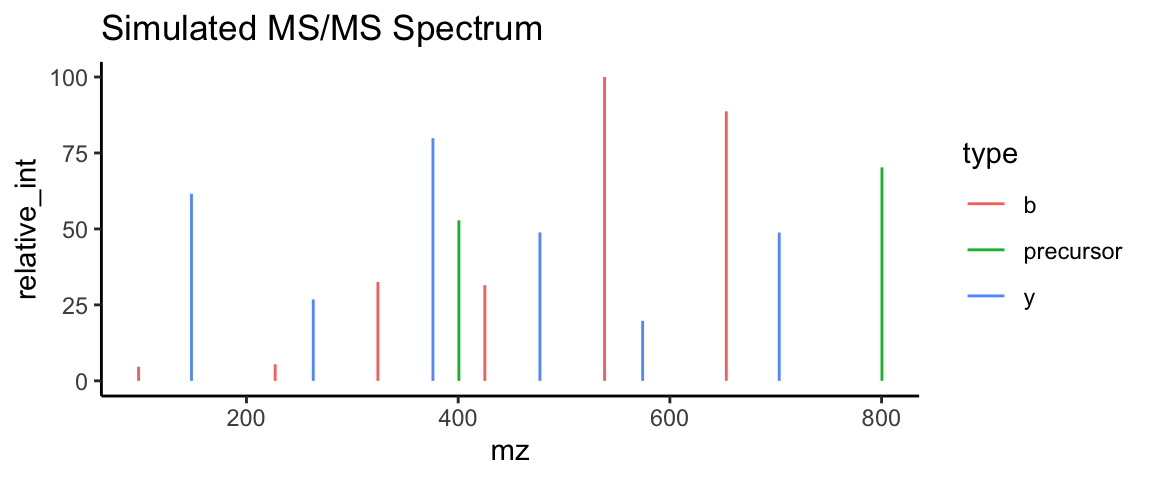
\includegraphics{_main_files/figure-latex/unnamed-chunk-9-1.pdf}

One of the key benefits of using the Tidyverse is the standardization of syntax and functions across each package. This means that once you learn the basics of one package, you can easily switch to another package and be confident in your ability to use it. This makes it easier to create reproducible code and improves the efficiency of your data analysis.

The Tidyverse is widely used in the R community and is a valuable tool for any data scientist or analyst working with R. It is especially useful for those who need to manipulate and visualize data quickly and efficiently, without sacrificing accuracy. Whether you are new to R or an experienced user, the Tidyverse is a must-have tool in your data analysis toolkit.

\hypertarget{mass-spectrometry-specific-packages}{%
\subsection{Mass Spectrometry Specific Packages}\label{mass-spectrometry-specific-packages}}

This book, while providing a beginners level guide to R programming, also introduces several mass spectrometry-specific packages in many of the code examples. While these examples may only touch on some of their functions, the last chapter is dedicated to a more formal, albeit not comprehensive introduction to many of these packages. For example the \texttt{mzR} package, which enables users to read and process mass spectrometry data, as well as the \texttt{xcms} package, which is used for preprocessing and feature detection. Additionally, the book introduces the \texttt{MSnbase} package, which provides a framework for quantitative and qualitative analysis of mass spectrometry data, and the \texttt{MSstats} package, which is used for statistical analysis of quantitative proteomics experiments. Lastly, the book covers the \texttt{tidyproteomic}s package, which provides a collection of tools for analyzing post-analysis quantitative proteomics data using a framework similar to the \texttt{tidyverse}.

\hypertarget{the-basics}{%
\chapter{The Basics}\label{the-basics}}

Welcome to the R Book! In this chapter, we will explore the basics of R, a powerful programming language used for statistical computing and graphics.

At its most fundamental level, R is a calculator capable of performing simple, and complex, mathematical operations. It can read and write data to and from files, manipulate the data, calculate summaries and plot visual representations of the data. Essentially, it is a programmatic version of a spreadsheet program.

However, R is much more than just a calculator. It is also a platform for conducting complex analyses, statistical evaluations, predictive inferencing, and machine learning. With R, you can explore and visualize data in a variety of ways, perform advanced statistical analyses, and build predictive models.

In this chapter, we will start by examining the simplest operations of R. We will cover basic arithmetic, working with variables, and creating basic plots. By the end of this chapter, you will have a solid understanding of the fundamentals of R and be ready to tackle more complex topics.

So, let's get started!

\begin{infobox}{skill}
At the end of this chapter you should be able to:\\
1. Understand R's syntax, variables, operators and functions\\
2. Create and edit a project in RStudio\\


\end{infobox}

\hypertarget{reserved-words}{%
\section{Reserved Words}\label{reserved-words}}

As we begin our journey, it's important to keep in mind that there are certain reserved words that carry a special meaning and cannot be used as identifiers. These words have been set aside by the R programming language, and using them as variable names or function names could lead to errors in your code.

Therefore, before we dive too deeply into our R programming endeavors, let's take a moment to familiarize ourselves with these reserved words. This will help us avoid potential issues down the road and ensure that our code runs smoothly.

\begin{Shaded}
\begin{Highlighting}[]
\CommentTok{\# to read more about them type}
\NormalTok{?reserved}
\end{Highlighting}
\end{Shaded}

\begin{longtable}[]{@{}
  >{\raggedright\arraybackslash}p{(\columnwidth - 2\tabcolsep) * \real{0.4167}}
  >{\raggedright\arraybackslash}p{(\columnwidth - 2\tabcolsep) * \real{0.5833}}@{}}
\toprule\noalign{}
\begin{minipage}[b]{\linewidth}\raggedright
Word
\end{minipage} & \begin{minipage}[b]{\linewidth}\raggedright
Use
\end{minipage} \\
\midrule\noalign{}
\endhead
\bottomrule\noalign{}
\endlastfoot
\texttt{if}, \texttt{else} & flow control, part of the if-then-else statement \\
\texttt{for}, \texttt{repeat}, \texttt{while}, \texttt{break}, \texttt{next} & flow control, part of the for-loop statement \\
\texttt{function} & basis for defining new algorithms \\
\texttt{TRUE}, \texttt{FALSE} & Boolean logic values \\
\texttt{NULL} & an undefined value \\
\texttt{Inf} , \texttt{-Inf} & an infinite value (eg. \texttt{1/0} ) \\
\texttt{NaN} & `not a number' \\
\texttt{NA} & a missing value indicator \\
\end{longtable}

\begin{infobox}{note}
A \texttt{Null} results when a value is missing and could be a \emph{string} or a \emph{numeric}, where as a NA results when a known value, such as in a column of numbers, is missing.

\end{infobox}

\hypertarget{syntax}{%
\section{Syntax}\label{syntax}}

Welcome to the R Book! Whether you're just starting out or a seasoned pro, understanding the different components of R code is essential for writing high-quality, efficient R programs. In this section, we'll take a deep dive into the various components of R code that you should be familiar with.

R input is composed of typed characters that represent different parts of a process or mathematical operation. These characters come together to form what we call R code. It's important to note that R code is not just a random collection of characters - each character serves a specific purpose and contributes to the larger structure of the code. As such, understanding the different components of R code is key to writing effective and efficient R programs.

So, what are these different components of R code? Below, we've provided some examples to help you get started:

\begin{longtable}[]{@{}
  >{\raggedright\arraybackslash}p{(\columnwidth - 2\tabcolsep) * \real{0.3780}}
  >{\raggedright\arraybackslash}p{(\columnwidth - 2\tabcolsep) * \real{0.6220}}@{}}
\toprule\noalign{}
\endhead
\bottomrule\noalign{}
\endlastfoot
\ref{comments} comments & \texttt{\#\ this\ is\ an\ important\ note} \\
\ref{strings} strings & \texttt{"letters"} or \texttt{"numbers"} in quotes \\
\ref{numbers} numbers & \texttt{1} integers or \texttt{1.000002} floats \\
\ref{operators} operators & \texttt{+}, \texttt{-}, \texttt{/}, \texttt{*}, \ldots{} \\
\ref{variables} variables & \texttt{var\ \textless{}-\ 2} containers for information \\
\ref{statements} statements & \texttt{==} exactly the same, \texttt{!=} not the same \\
\ref{functions} functions & \texttt{add(x,\ y)} complex code in a convenient wrapper \\
\end{longtable}

By understanding these different components of R code, you'll be well on your way to writing effective and efficient R programs. So let's dive in and get started!

\begin{Shaded}
\begin{Highlighting}[]
\CommentTok{\# adding two numbers here and storing it as a variable}
\NormalTok{four }\OtherTok{\textless{}{-}} \DecValTok{2} \SpecialCharTok{+} \DecValTok{2}

\CommentTok{\# using the function \textquotesingle{}cat\textquotesingle{} to print out my variable along with some text}
\FunctionTok{cat}\NormalTok{(}\StringTok{"my number is "}\NormalTok{, four)}
\end{Highlighting}
\end{Shaded}

\begin{verbatim}
## my number is  4
\end{verbatim}

\begin{infobox}{note}
R does not have an line ending character such as \texttt{;} in java, PHP or C++\_

\end{infobox}

\hypertarget{comments}{%
\subsection{Comments}\label{comments}}

Comments are essential parts of the code you will write. They help explain why you are taking a certain approach to the problem, either for you to remember at a later time or for a colleague. Comments in other coding languages, including R package development, can become quite expressive, representing parts and structures to a larger documentation effort. Here, however, comments are just simple text that gets ignored by the R interpreter. You can put anything you want in comments.

\begin{Shaded}
\begin{Highlighting}[]
\NormalTok{oops, not a comment}
\end{Highlighting}
\end{Shaded}

\begin{Shaded}
\begin{Highlighting}[]
\CommentTok{\# This is a comment}

\CommentTok{\# and here a comment tag is used to ignore legitimate R code}
\CommentTok{\# four \textless{}{-} 2 + 2 }
\NormalTok{four }\OtherTok{\textless{}{-}} \DecValTok{2} \SpecialCharTok{*} \DecValTok{2}
\end{Highlighting}
\end{Shaded}

\hypertarget{strings}{%
\subsection{Strings}\label{strings}}

Strings are essentially a sequence of characters, consisting of letters or numbers. They are commonly used in programming languages and are used to represent text-based data. A string can be as simple as a single character, such as ``A'', or it can be a longer sequence of characters such as ``Hello, World!''. Strings are often used to store data that requires text manipulation, such as usernames, passwords, and email addresses. In contrast to words, which are made up of a specific combination of letters to represent a linguistic term, strings do not follow any specific rules of composition and can be a random or semi-random sequence of characters.

\begin{Shaded}
\begin{Highlighting}[]
\CommentTok{\# a string can be a word, this is a string variable}
\NormalTok{three }\OtherTok{\textless{}{-}} \DecValTok{1} \SpecialCharTok{+} \DecValTok{2}
\CommentTok{\# or an abbreviation, this is a variable (thr) representing the string "three"}
\NormalTok{thr }\OtherTok{\textless{}{-}} \StringTok{"three"} 
\CommentTok{\# a mass spec reference}
\NormalTok{peptide }\OtherTok{\textless{}{-}} \StringTok{"QWERTK"}
\CommentTok{\# or an abbreviated variable}
\NormalTok{pep }\OtherTok{\textless{}{-}} \StringTok{"QWERTK"}
\end{Highlighting}
\end{Shaded}

When working with R programming language, it is essential to note that strings play a crucial role in the syntax used. Strings, which define text characters, are used to represent data in R, and they must be enclosed in quotes. Failure to do so will result in the interpreter assuming that you are referring to a variable that is not enclosed in quotes.

For instance, in the example above, the \texttt{peptide} variable contains the string of letters representing the peptide amino acid sequence \texttt{"QWERTK"}. However, it is essential to note that there are no strict rules for how strings and variables are composed, except that variables \textbf{cannot} start with a number.

\begin{Shaded}
\begin{Highlighting}[]
\CommentTok{\# permitted}
\NormalTok{b4 }\OtherTok{\textless{}{-}} \DecValTok{1} \SpecialCharTok{+} \DecValTok{3}
\CommentTok{\# not permitted}
\NormalTok{4b }\OtherTok{\textless{}{-}} \DecValTok{1} \SpecialCharTok{+} \FloatTok{3.} \DocumentationTok{\#\# Error: unexpected symbol in "4b"}
\end{Highlighting}
\end{Shaded}

There are however, conventions that you can follow when constructing variable names that aid in the readability of the code and convey information about the contents. This is especially useful in long code blocks, or, when the code becomes more complex and divested across several files. For example:

\begin{Shaded}
\begin{Highlighting}[]
\CommentTok{\# a string containing a peptide sequence}
\NormalTok{str\_pep }\OtherTok{\textless{}{-}} \StringTok{"QWERTK"}

\CommentTok{\# a data table of m/z values and their identifications}
\NormalTok{tbl\_mz\_ids }\OtherTok{\textless{}{-}} \FunctionTok{read\_csv}\NormalTok{(}\StringTok{"somefile.csv"}\NormalTok{)}
\end{Highlighting}
\end{Shaded}

To learn more about and follow specific conventions, explore the following resources:

\begin{itemize}
\item
  \href{http://adv-r.had.co.nz/Style.html}{Hadley Wickham's Style Guide}
\item
  \href{https://google.github.io/styleguide/Rguide.html}{Google's style Guide}
\item
  \href{https://style.tidyverse.org/}{The tidyverse style guide}
\end{itemize}

\hypertarget{numbers}{%
\subsection{Numbers}\label{numbers}}

Numbers are the foundation upon which all data analysis is built. Without numbers, we would not be able to perform calculations, identify patterns, or draw conclusions from our data. In the programming language R, there are two main types of numbers: \texttt{integers} and \texttt{floats}. An integer is a whole number with no decimal places, while a float is a number with decimal places. Understanding the difference between these two types of numbers is essential for accurate numerical analysis.

In R, integers are represented as whole numbers, such as 1, 2, 3, and so on, while floats are represented with a decimal point, such as 1.5, 2.75, and so on. It is important to note that integers occupy less space in memory than floats, which can be a consideration when working with large datasets. This means that when possible, it is generally better to use integers over floats in R, as they are more efficient and can improve the overall performance of your code.

\begin{Shaded}
\begin{Highlighting}[]
\CommentTok{\# integers}
\DecValTok{1}\NormalTok{,  }\DecValTok{12345}\NormalTok{, }\SpecialCharTok{{-}}\DecValTok{17}\NormalTok{, }\DecValTok{0}
\end{Highlighting}
\end{Shaded}

Numbers are the foundation upon which all data analysis is built. Without numbers, we would not be able to perform calculations, identify patterns, or draw conclusions from our data. In the programming language R, there are two main types of numbers: \texttt{integers} and \texttt{floats}.

An integer is a whole number with no decimal places, while a float is a number with decimal places. In most programming languages, including R, integers are represented as whole numbers, such as 1, 2, 3, and so on, while floats are represented with a decimal point, such as 1.5, 2.75, and so on.

It is essential to understand the difference between these two types of numbers for accurate numerical analysis. While integers can only represent whole numbers, floats can represent fractions and decimals. Thus, if you need to represent a number that is not a whole number, you should use a float.

Moreover, it is important to note that integers occupy less space in memory than floats. This can be a consideration when working with large datasets, especially when the whole number is enough to represent the data. Therefore, when possible, it is generally better to use integers over floats in R, as they are more efficient and can improve the overall performance of your code.

\begin{Shaded}
\begin{Highlighting}[]
\CommentTok{\# floats}
\NormalTok{significand }\OtherTok{\textless{}{-}} \DecValTok{12345}
\NormalTok{exponent }\OtherTok{\textless{}{-}} \SpecialCharTok{{-}}\DecValTok{3}
\NormalTok{base }\OtherTok{\textless{}{-}} \DecValTok{10}

\CommentTok{\# 12.345 = 12345 * 10\^{}{-}3}
\NormalTok{significand }\SpecialCharTok{*}\NormalTok{ base }\SpecialCharTok{\^{}}\NormalTok{ exponent}
\end{Highlighting}
\end{Shaded}

\hypertarget{operators}{%
\subsection{Operators}\label{operators}}

Operators are fundamental components of programming that enable us to manipulate and process various data types. They are symbols that perform a specific action on one or more operands, which could be numeric values, variables, or even strings. Most commonly these symbols allow us to perform basic arithmetic operations such as addition, subtraction, multiplication, and division on numeric values, as well as more complex mathematical operations like exponentiation and modulus.

In addition to numeric values, operators can also manipulate string variables. For instance, we can use concatenation operators to join two or more strings together, which is particularly useful when working with text data. By utilizing operators, we can perform powerful operations that allow us to build complex programs and applications that can handle large amounts of data. Operators play a crucial role in programming, as they allow us to manipulate data in a way that would be difficult or impossible to achieve otherwise.

At their very basic, operators allow you to perform \textbf{calculations} ..

\begin{Shaded}
\begin{Highlighting}[]
\DecValTok{1} \SpecialCharTok{+} \DecValTok{2}
\end{Highlighting}
\end{Shaded}

\begin{verbatim}
## [1] 3
\end{verbatim}

\begin{Shaded}
\begin{Highlighting}[]
\DecValTok{1} \SpecialCharTok{/} \DecValTok{2}
\end{Highlighting}
\end{Shaded}

\begin{verbatim}
## [1] 0.5
\end{verbatim}

.. \textbf{assign} values to string variables ..

\begin{Shaded}
\begin{Highlighting}[]
\NormalTok{myvar }\OtherTok{\textless{}{-}} \DecValTok{1}
\end{Highlighting}
\end{Shaded}

.. and \textbf{compare} values.

\begin{Shaded}
\begin{Highlighting}[]
\DecValTok{1} \SpecialCharTok{==}\NormalTok{ myvar}
\end{Highlighting}
\end{Shaded}

\begin{verbatim}
## [1] TRUE
\end{verbatim}

\begin{Shaded}
\begin{Highlighting}[]
\DecValTok{2} \SpecialCharTok{!=}\NormalTok{ myvar }\SpecialCharTok{+}\NormalTok{ myvar}
\end{Highlighting}
\end{Shaded}

\begin{verbatim}
## [1] FALSE
\end{verbatim}

Here is a table summarizing of some common operators in R.

\begin{longtable}[]{@{}
  >{\raggedright\arraybackslash}p{(\columnwidth - 6\tabcolsep) * \real{0.1111}}
  >{\raggedright\arraybackslash}p{(\columnwidth - 6\tabcolsep) * \real{0.1709}}
  >{\raggedright\arraybackslash}p{(\columnwidth - 6\tabcolsep) * \real{0.3932}}
  >{\raggedright\arraybackslash}p{(\columnwidth - 6\tabcolsep) * \real{0.3077}}@{}}
\toprule\noalign{}
\begin{minipage}[b]{\linewidth}\raggedright
Operator
\end{minipage} & \begin{minipage}[b]{\linewidth}\raggedright
Name
\end{minipage} & \begin{minipage}[b]{\linewidth}\raggedright
Description
\end{minipage} & \begin{minipage}[b]{\linewidth}\raggedright
Example
\end{minipage} \\
\midrule\noalign{}
\endhead
\bottomrule\noalign{}
\endlastfoot
\texttt{\textless{}-} & assignmnet & assigns numerics and functions to variables & \texttt{x\ \textless{}-\ 1} x now has the value of 1 \\
\texttt{+} & addition & adds two numbers & \texttt{1\ +\ 2} = \texttt{3} \\
\texttt{-} & subtraction & subtracts two numbers & \texttt{1\ -\ 2} = \texttt{-1} \\
\texttt{*} & multplication & multiplies two numbers & \texttt{1\ *\ 2} = \texttt{2} \\
\texttt{/} & division & divides two numbers & \texttt{1\ /\ 2} = \texttt{0.5} \\
\texttt{\^{}} & power or exponent & raises one number to the power of the other & \texttt{1\ \^{}\ 2} = \texttt{1} \\
\texttt{=} & equals & also an assignment operator & \texttt{x\ =\ 1} x now has the value of 1 \\
\texttt{==} & double equals & performs a comparison (exactly equal) & \texttt{1\ ==\ 1} = \texttt{TRUE} \\
\texttt{!=} & not equals & performs a negative comparison (not equal) & \texttt{1\ !=\ 2} = \texttt{TRUE} \\
\texttt{\%\%} & modulus & provides the remainder after division & \texttt{5\ \%\%\ 2} = \texttt{1} \\
\end{longtable}

\begin{infobox}{note}
Remember order of operations (PEMDAS): Parentheses, Exponents, Multiplication and Division (from left to right), Addition and Subtraction (from left to right).

\end{infobox}

\hypertarget{variables}{%
\subsection{Variables}\label{variables}}

In programming, variables are essential elements used to store information that can in essence \textbf{vary}. They come in handy when we need to manipulate or retrieve the information stored in them.

Variables can be thought of as containers that can store any kind of information, such as letters, words, numbers, or text strings. They are flexible enough to hold different types of data, and we can use them to store all sorts of information.

One of the most significant advantages of using variables is that we can refer to them repeatedly to retrieve the information stored in them. We can also manipulate the information stored in them with an operation or replace it with an assignment. Variables are a powerful tool in programming that allows us to store and retrieve information, manipulate it, and perform various operations on it.

\begin{Shaded}
\begin{Highlighting}[]
\CommentTok{\# create two viables and assign values to each}
\NormalTok{var\_a }\OtherTok{\textless{}{-}} \DecValTok{1}
\NormalTok{var\_b }\OtherTok{\textless{}{-}} \FloatTok{3.14}

\NormalTok{var\_a }\SpecialCharTok{+}\NormalTok{ var\_b}
\end{Highlighting}
\end{Shaded}

\begin{verbatim}
## [1] 4.14
\end{verbatim}

R even has some intrinsic variables that come in handy, like \emph{pi}.

\begin{Shaded}
\begin{Highlighting}[]
\NormalTok{pi}
\end{Highlighting}
\end{Shaded}

\begin{verbatim}
## [1] 3.141593
\end{verbatim}

\begin{infobox}{note}
In R it is easy to overwrite existing variables, either initalized by R or created by you, causing error and confusion

\end{infobox}

\begin{Shaded}
\begin{Highlighting}[]
\NormalTok{pi }\OtherTok{\textless{}{-}} \FloatTok{9.876543}
\NormalTok{pi}
\end{Highlighting}
\end{Shaded}

\begin{verbatim}
## [1] 9.876543
\end{verbatim}

\hypertarget{statements}{%
\subsection{Statements}\label{statements}}

Using a comparison operator, you can make logical comparisons called statements.

\begin{longtable}[]{@{}
  >{\raggedright\arraybackslash}p{(\columnwidth - 4\tabcolsep) * \real{0.1120}}
  >{\raggedright\arraybackslash}p{(\columnwidth - 4\tabcolsep) * \real{0.6400}}
  >{\raggedright\arraybackslash}p{(\columnwidth - 4\tabcolsep) * \real{0.2400}}@{}}
\toprule\noalign{}
\begin{minipage}[b]{\linewidth}\raggedright
Operator
\end{minipage} & \begin{minipage}[b]{\linewidth}\raggedright
Description
\end{minipage} & \begin{minipage}[b]{\linewidth}\raggedright
Example
\end{minipage} \\
\midrule\noalign{}
\endhead
\bottomrule\noalign{}
\endlastfoot
\texttt{\textbar{}} & an either \textbf{or} comparison, \texttt{TRUE} if both are true \texttt{FALSE} if one is false. & \texttt{1\ ==\ 1\ \textbar{}\ 1\ !=\ 2} = \texttt{TRUE}

\texttt{1\ ==\ 1\ \textbar{}\ 1\ ==\ 2} = \texttt{FALSE} \\
\texttt{\&} & a comparison where \textbf{both} must be \texttt{TRUE} & \texttt{1\ ==\ 1\ \&\ 1\ !=\ 2} = \texttt{TRUE}

\texttt{1\ ==\ 1\ \&\ 1\ !=\ 2} = \texttt{FALSE} \\
\end{longtable}

\begin{quote}
\textbf{NOTE}\\
\emph{there are also the double operators \textbar\textbar{} and \&\&, these are intended to work as flow control operators and stop at the first condition met. In the most recent versions of R, the double operators will error out if a vector is applied.}
\end{quote}

\hypertarget{functions}{%
\subsection{Functions}\label{functions}}

In programming, a function is a type of operator that performs a specific task and can accept additional information or parameters. In fact, all operators are functions in a sense, as they take inputs and produce outputs.

The R programming language has a special class of operators called ``binary infix'' operators. Infix means ``in between,'' and these operators are placed in between two inputs. These operators have a unique syntax that may confuse beginners, but they are essential for more complex operations in R.

Now, you may wonder why we are discussing these esoteric aspects of R in a beginner's book. The reason is that understanding these unique features of the language can give you a better understanding of what the R programming language is doing, how it is structured, and how you can relate to it. It is important to have a solid foundation in the basics of any language, but gaining a deeper understanding of its more complex elements can help you become a more proficient programmer.

So, while binary infix operators may seem like an advanced topic, they are an essential part of the R language and can help you unlock its full potential.

\begin{Shaded}
\begin{Highlighting}[]
\DecValTok{1} \SpecialCharTok{+} \DecValTok{2}          \CommentTok{\# as an infix operator }
\end{Highlighting}
\end{Shaded}

\begin{verbatim}
## [1] 3
\end{verbatim}

\begin{Shaded}
\begin{Highlighting}[]
\StringTok{\textasciigrave{}}\AttributeTok{+}\StringTok{\textasciigrave{}}\NormalTok{(}\DecValTok{1}\NormalTok{,}\DecValTok{2}\NormalTok{)       }\CommentTok{\# as the function}
\end{Highlighting}
\end{Shaded}

\begin{verbatim}
## [1] 3
\end{verbatim}

\begin{Shaded}
\begin{Highlighting}[]
\FunctionTok{sum}\NormalTok{(}\DecValTok{1}\NormalTok{,}\DecValTok{2}\NormalTok{)       }\CommentTok{\# same result just using a named function}
\end{Highlighting}
\end{Shaded}

\begin{verbatim}
## [1] 3
\end{verbatim}

\begin{Shaded}
\begin{Highlighting}[]
\FunctionTok{sum}\NormalTok{(}\DecValTok{1}\NormalTok{,}\DecValTok{2}\NormalTok{,}\DecValTok{3}\NormalTok{,}\DecValTok{4}\NormalTok{,}\DecValTok{5}\NormalTok{) }\CommentTok{\# this function however can take in more than 2 values}
\end{Highlighting}
\end{Shaded}

\begin{verbatim}
## [1] 15
\end{verbatim}

We can even create a user defined infix operator \ldots{}

\begin{Shaded}
\begin{Highlighting}[]
\StringTok{\textasciigrave{}}\AttributeTok{\%zyx\%}\StringTok{\textasciigrave{}} \OtherTok{\textless{}{-}} \ControlFlowTok{function}\NormalTok{(a,b) \{ a }\SpecialCharTok{+}\NormalTok{ b \}}
\DecValTok{1} \SpecialCharTok{\%zyx\%} \DecValTok{2}
\end{Highlighting}
\end{Shaded}

\begin{verbatim}
## [1] 3
\end{verbatim}

\ldots{} or just a normal function.

\begin{Shaded}
\begin{Highlighting}[]
\NormalTok{zyx }\OtherTok{\textless{}{-}} \ControlFlowTok{function}\NormalTok{(a,b) \{ a }\SpecialCharTok{+}\NormalTok{ b \}}
\FunctionTok{zyx}\NormalTok{(}\DecValTok{1}\NormalTok{,}\DecValTok{2}\NormalTok{)}
\end{Highlighting}
\end{Shaded}

\begin{verbatim}
## [1] 3
\end{verbatim}

The notion of an infix operator you and ignore for the most part. But, we will see it again when diving into the \texttt{tidyverse} - a collection of arguably the most powerful data manipulation packages you will encounter. For now, lets move on with more about \texttt{functions()}.

\hypertarget{flow-control}{%
\section{Flow-Control}\label{flow-control}}

\hypertarget{if-else-statements}{%
\subsection{If-Else Statements}\label{if-else-statements}}

\hypertarget{loops}{%
\subsection{Loops}\label{loops}}

\hypertarget{for}{%
\subsubsection{For}\label{for}}

\hypertarget{while}{%
\subsubsection{While}\label{while}}

\hypertarget{projects}{%
\section{Projects}\label{projects}}

Project are how RStudio organizes your work. Think of project as singular goal oriented collection. There are no rules but some basic organizational tips should help simplify your project.

\hypertarget{creating}{%
\subsection{Creating}\label{creating}}

Creating a new project is very forgiving, you can create a new directory with a project name, or create a project out of an existing directory.

Either 1. Click on the drop down in the top right 2. OR: Under the menu item select \texttt{File\ \textgreater{}\ New\ Project}

In the \texttt{New\ Project\ Wizard} select \texttt{New\ Directory\ \textgreater{}\ New\ Project}, enter the name of the project and click \texttt{Create\ Project}.

\begin{figure}
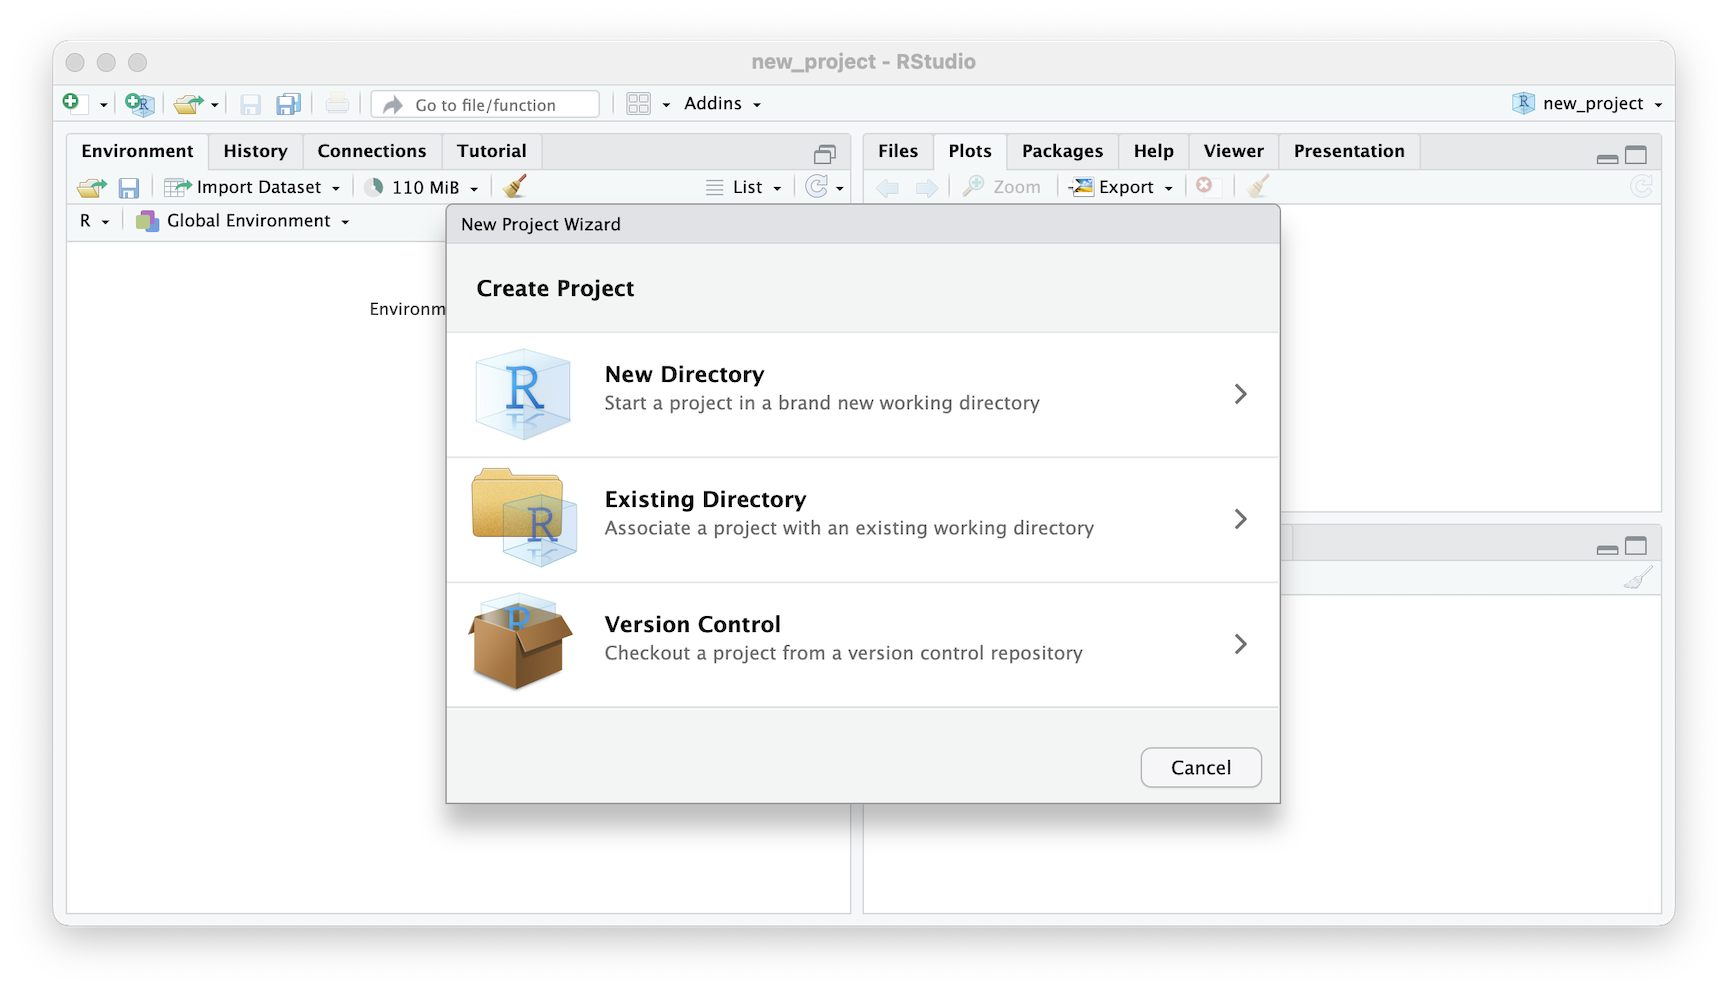
\includegraphics[width=30.72in]{images/03_021_new_project_01} \caption{\label{fig:3201}RStudio Create New Project}\label{fig:3201}
\end{figure}
\begin{figure}
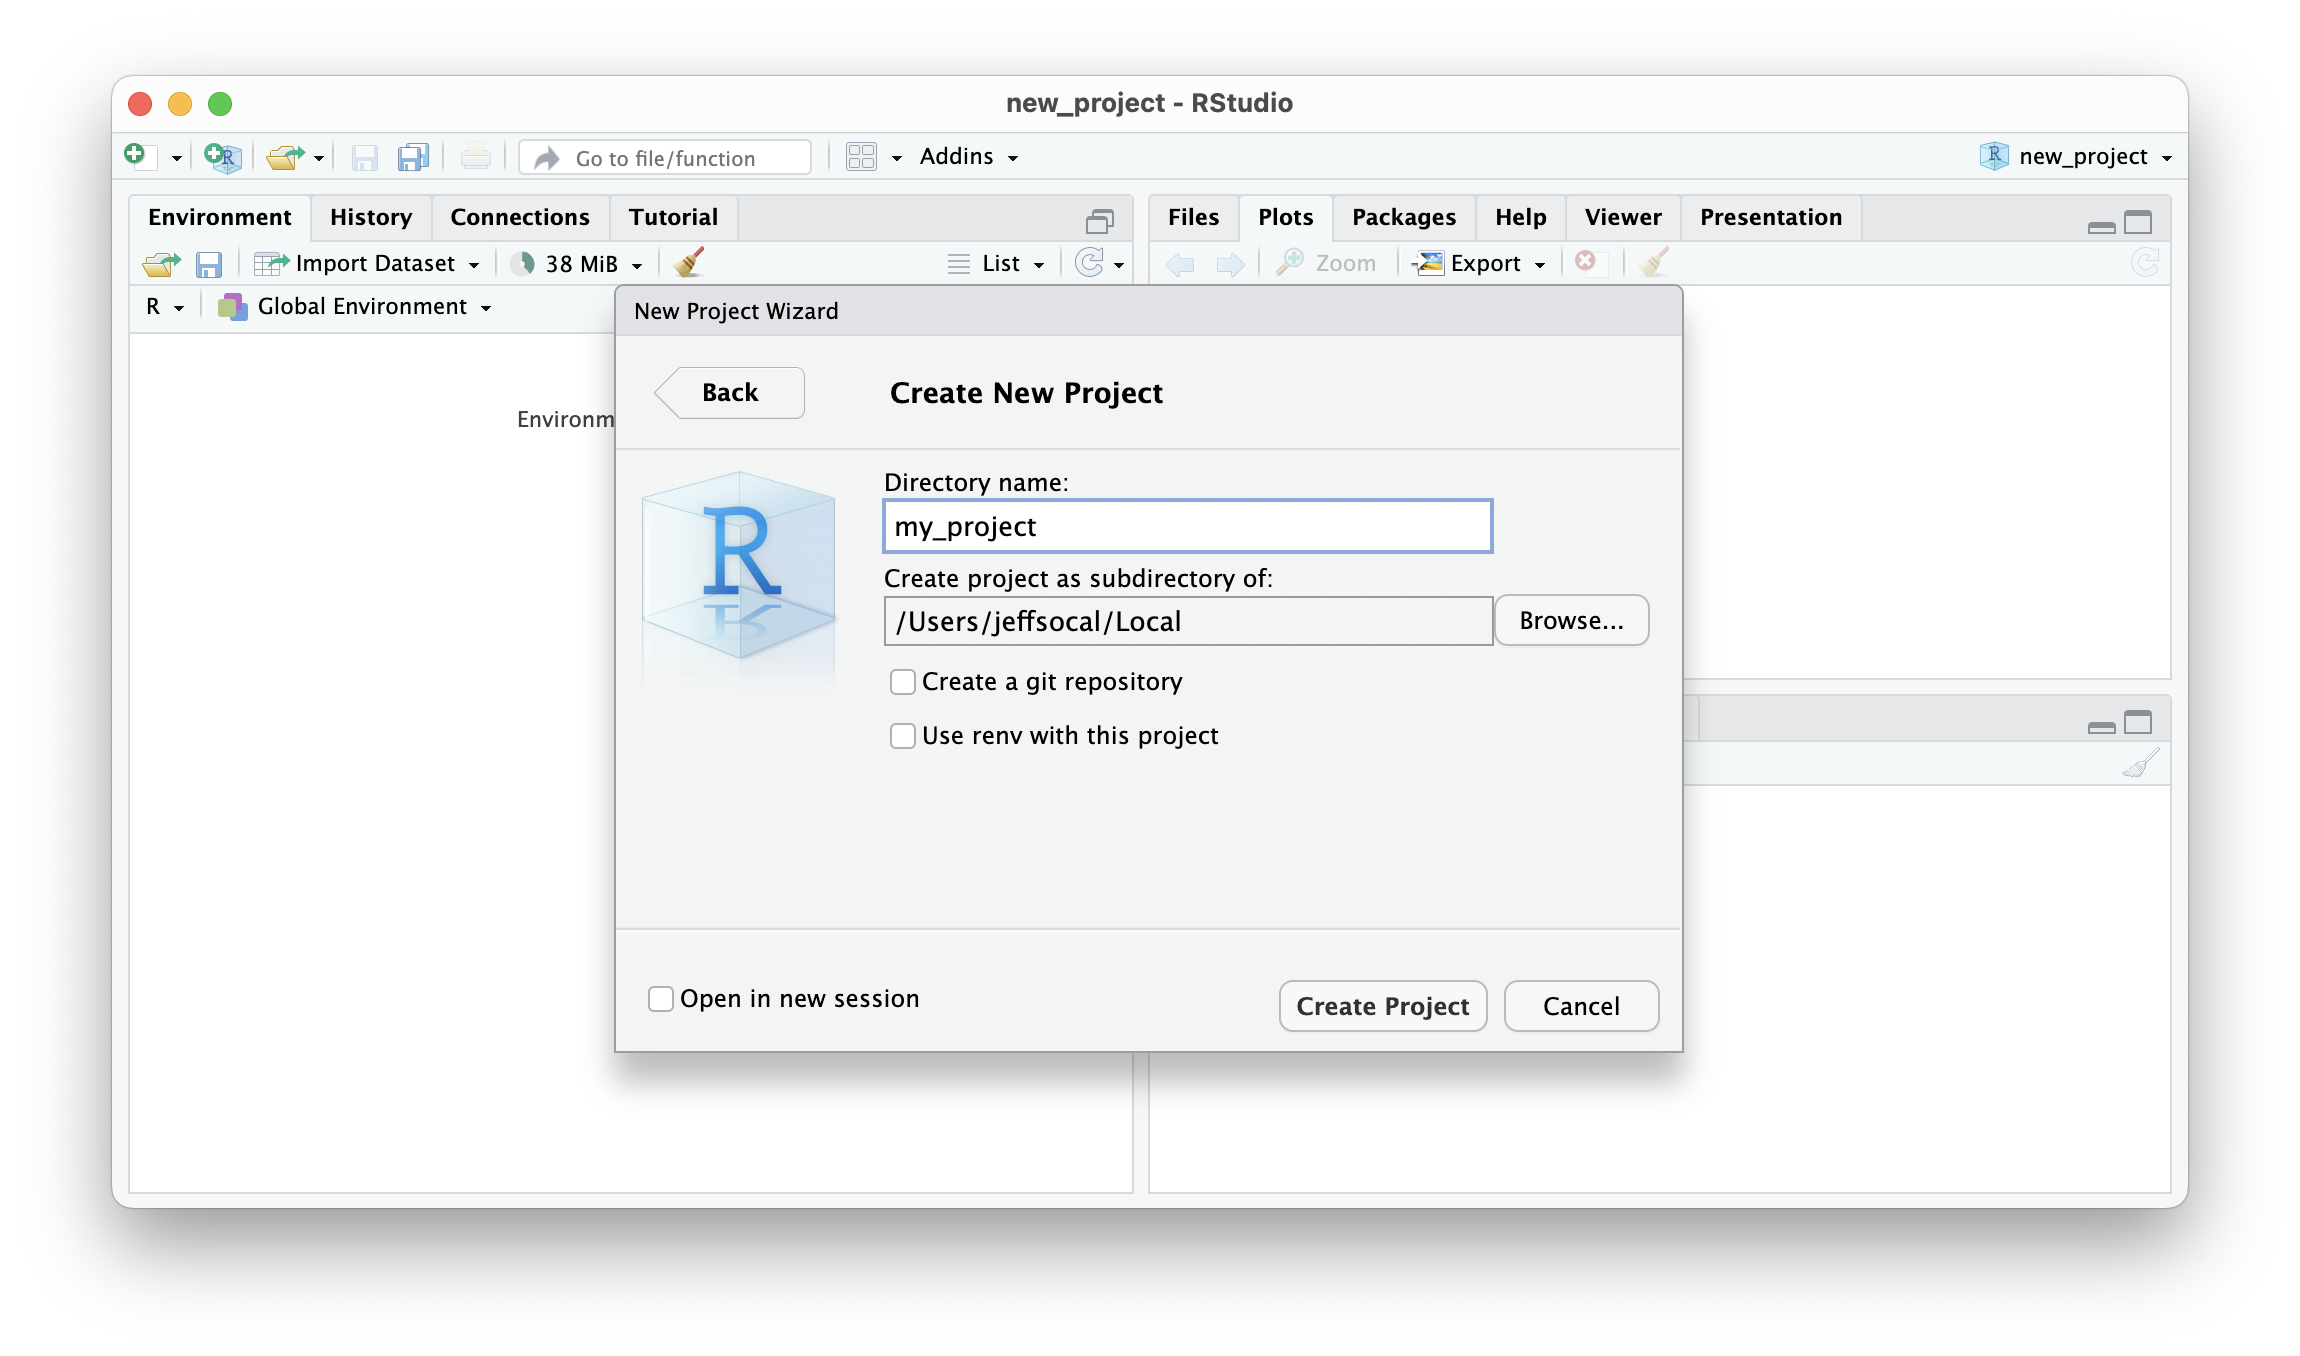
\includegraphics[width=31.94in]{images/03_021_new_project_02} \caption{\label{fig:3202}RStudio Create New Project}\label{fig:3202}
\end{figure}

\hypertarget{editing}{%
\subsection{Editing}\label{editing}}

\hypertarget{organizing}{%
\subsection{Organizing}\label{organizing}}

\hypertarget{data}{%
\subsubsection{Data}\label{data}}

\hypertarget{scripts}{%
\subsubsection{Scripts}\label{scripts}}

\hypertarget{results}{%
\subsubsection{Results}\label{results}}

\hypertarget{tables}{%
\paragraph{Tables}\label{tables}}

\hypertarget{plots}{%
\paragraph{Plots}\label{plots}}

\hypertarget{exercises}{%
\section*{Exercises}\label{exercises}}
\addcontentsline{toc}{section}{Exercises}

\begin{enumerate}
\def\labelenumi{\arabic{enumi}.}
\tightlist
\item
  Calculate the sum of 2 and 3.
\end{enumerate}

\begin{verbatim}
## [1] 5
\end{verbatim}

\begin{enumerate}
\def\labelenumi{\arabic{enumi}.}
\setcounter{enumi}{1}
\tightlist
\item
  Evaluate if 0.5 is equal to 1 divided by 2.
\end{enumerate}

\begin{verbatim}
## [1] TRUE
\end{verbatim}

\begin{enumerate}
\def\labelenumi{\arabic{enumi}.}
\setcounter{enumi}{2}
\tightlist
\item
  Test if 3 is an even number. Hint, use the modulus operator and a comparison operator.
\end{enumerate}

\begin{verbatim}
## [1] FALSE
\end{verbatim}

\begin{enumerate}
\def\labelenumi{\arabic{enumi}.}
\setcounter{enumi}{3}
\tightlist
\item
  Create a function to test if a value is even resulting in \texttt{TRUE} or \texttt{FALSE}.
\end{enumerate}

\begin{Shaded}
\begin{Highlighting}[]
\FunctionTok{even}\NormalTok{(}\DecValTok{3}\NormalTok{)}
\end{Highlighting}
\end{Shaded}

\begin{verbatim}
## [1] FALSE
\end{verbatim}

\begin{enumerate}
\def\labelenumi{\arabic{enumi}.}
\setcounter{enumi}{3}
\tightlist
\item
  Create a function to test or \emph{even} or \emph{odd} by returning a string.
\end{enumerate}

\begin{Shaded}
\begin{Highlighting}[]
\FunctionTok{oddeven}\NormalTok{(}\DecValTok{3}\NormalTok{)}
\end{Highlighting}
\end{Shaded}

\begin{verbatim}
## [1] "odd"
\end{verbatim}

\hypertarget{data-structures}{%
\chapter{Data Structures}\label{data-structures}}

The R programming environment includes four basic types of data structures that increase in complexity: \texttt{variable}, \texttt{vector}, \texttt{matrix}, and \texttt{list}. Additionally there is the \texttt{data.frame} while and independent data structure, it is essentially derived from the \texttt{matrix}.

\begin{infobox}{skill}
At the end of this chapter you should be able to:\\
1. Understand the 5 most common data structures\\
2. Understand the data structure lineage\\
3. Access given subsets of a multi-variable data object\\


\end{infobox}

\hfill\break
This book introduced variables briefly in \ref{syntax}. Here, we will expand on that introduction. At its simplest, a variable can be thought of as a container that holds only a single thing, like a single stick of gum. A vector is an ordered, finite collection of variables, like a pack of gum. A matrix consists of columns of equally-sized vectors, similar to a vending machine for several flavors of gum packs. Mentally, you can think of them as a point, a line, and a square, respectively.

\begin{figure}

{\centering 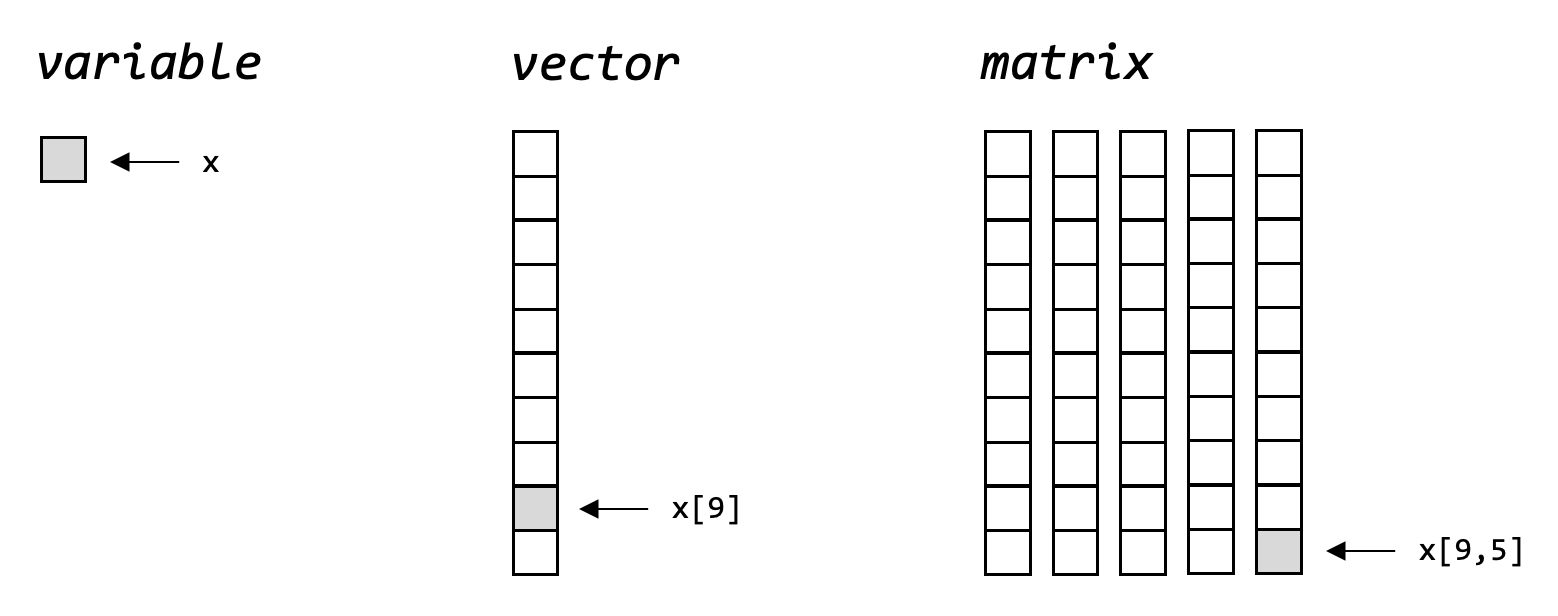
\includegraphics[width=0.67\linewidth]{images/04_001_data_structures} 

}

\caption{\label{fig:4001}R main data structures}\label{fig:4001}
\end{figure}

\hypertarget{variable}{%
\section{Variable}\label{variable}}

Again, a variable is the most basic information container, capable of holding only a single \emph{numeric} or \emph{string} value.

\begin{Shaded}
\begin{Highlighting}[]
\NormalTok{a }\OtherTok{\textless{}{-}} \DecValTok{1}
\end{Highlighting}
\end{Shaded}

\hypertarget{vector}{%
\section{Vector}\label{vector}}

A vector is simply a collection of variables of all the same type. In other programming languages these are called arrays, and can be more permissive allowing for different types of values to be stored together. In R this is not permitted, as vectors can only contain either numbers or strings. If a vector contains a single string value, this ``spoils'' the numbers in the vector, thus making them all strings.

\begin{Shaded}
\begin{Highlighting}[]
\CommentTok{\# permitted}
\NormalTok{a }\OtherTok{\textless{}{-}} \FunctionTok{c}\NormalTok{(}\DecValTok{1}\NormalTok{, }\DecValTok{2}\NormalTok{, }\DecValTok{3}\NormalTok{)}
\NormalTok{a}
\end{Highlighting}
\end{Shaded}

\begin{verbatim}
## [1] 1 2 3
\end{verbatim}

\begin{Shaded}
\begin{Highlighting}[]
\CommentTok{\# the numerical values of 1 and 3 are lost, and now only represented as strings}
\NormalTok{b }\OtherTok{\textless{}{-}} \FunctionTok{c}\NormalTok{(}\DecValTok{1}\NormalTok{, }\StringTok{\textquotesingle{}two\textquotesingle{}}\NormalTok{, }\DecValTok{3}\NormalTok{)}
\NormalTok{b}
\end{Highlighting}
\end{Shaded}

\begin{verbatim}
## [1] "1"   "two" "3"
\end{verbatim}

Vectors can be composed through various methods, either by concatenation with the \texttt{c()} function, as seen above, or using the range operator \texttt{:}. Note that the concatenation method allows for the non-sequential construction of variables, while the range operator constructs a vector of all sequential integers between the two values.

\begin{Shaded}
\begin{Highlighting}[]
\DecValTok{1}\SpecialCharTok{:}\DecValTok{3}
\end{Highlighting}
\end{Shaded}

\begin{verbatim}
## [1] 1 2 3
\end{verbatim}

There are also a handful of pre-populated vectors and functions for constructing patters.

\begin{Shaded}
\begin{Highlighting}[]
\CommentTok{\# all upper case letters}
\NormalTok{LETTERS}
\end{Highlighting}
\end{Shaded}

\begin{verbatim}
##  [1] "A" "B" "C" "D" "E" "F" "G" "H" "I" "J" "K" "L" "M" "N" "O" "P" "Q" "R" "S" "T" "U" "V" "W" "X" "Y" "Z"
\end{verbatim}

\begin{Shaded}
\begin{Highlighting}[]
\CommentTok{\# all lower case letters}
\NormalTok{letters}
\end{Highlighting}
\end{Shaded}

\begin{verbatim}
##  [1] "a" "b" "c" "d" "e" "f" "g" "h" "i" "j" "k" "l" "m" "n" "o" "p" "q" "r" "s" "t" "u" "v" "w" "x" "y" "z"
\end{verbatim}

\begin{Shaded}
\begin{Highlighting}[]
\CommentTok{\# a repetitive vector of the letter "a"}
\FunctionTok{rep}\NormalTok{(}\StringTok{\textquotesingle{}a\textquotesingle{}}\NormalTok{, }\DecValTok{5}\NormalTok{)}
\end{Highlighting}
\end{Shaded}

\begin{verbatim}
## [1] "a" "a" "a" "a" "a"
\end{verbatim}

\begin{Shaded}
\begin{Highlighting}[]
\CommentTok{\# a repetitive vector of a previous vector}
\FunctionTok{rep}\NormalTok{(b, }\DecValTok{2}\NormalTok{)}
\end{Highlighting}
\end{Shaded}

\begin{verbatim}
## [1] "1"   "two" "3"   "1"   "two" "3"
\end{verbatim}

\begin{Shaded}
\begin{Highlighting}[]
\CommentTok{\# a sequence of integers between two values, in this case reverse order}
\FunctionTok{seq}\NormalTok{(}\DecValTok{10}\NormalTok{, }\DecValTok{5}\NormalTok{)}
\end{Highlighting}
\end{Shaded}

\begin{verbatim}
## [1] 10  9  8  7  6  5
\end{verbatim}

\begin{Shaded}
\begin{Highlighting}[]
\CommentTok{\# same as above}
\DecValTok{10}\SpecialCharTok{:}\DecValTok{5}
\end{Highlighting}
\end{Shaded}

\begin{verbatim}
## [1] 10  9  8  7  6  5
\end{verbatim}

While variables don't require a referencing scheme, because they only contain a single value, vectors need to have some kind of referencing scheme, shown in \ref{fig:4001} as \texttt{x{[}9{]}} and illustrated in the following example.

\begin{infobox}{note}
Note the use of an integer vector to sub-select another vector based on position. R abides by the 1:N positional referencing, where as other programming languages refer to the first vector or array position as 0.\\
\strut \\
\emph{A good topic for a lively discussion with a computer scientist.}

\end{infobox}

\hfill\break

\begin{Shaded}
\begin{Highlighting}[]
\NormalTok{x }\OtherTok{\textless{}{-}}\NormalTok{ LETTERS}
\CommentTok{\# 3rd letter in the alphabet}
\NormalTok{x[}\DecValTok{3}\NormalTok{]}
\end{Highlighting}
\end{Shaded}

\begin{verbatim}
## [1] "C"
\end{verbatim}

\begin{Shaded}
\begin{Highlighting}[]
\CommentTok{\# the 9th, 10th, 11th and 12th letters in the alphabet}
\NormalTok{x[}\DecValTok{9}\SpecialCharTok{:}\DecValTok{12}\NormalTok{]}
\end{Highlighting}
\end{Shaded}

\begin{verbatim}
## [1] "I" "J" "K" "L"
\end{verbatim}

\begin{Shaded}
\begin{Highlighting}[]
\CommentTok{\# the 1st, 5th, 10th letters in the alphabet}
\NormalTok{x[}\FunctionTok{c}\NormalTok{(}\DecValTok{1}\NormalTok{,}\DecValTok{5}\NormalTok{,}\DecValTok{10}\NormalTok{)]}
\end{Highlighting}
\end{Shaded}

\begin{verbatim}
## [1] "A" "E" "J"
\end{verbatim}

Numerical vectors can be operated on simultaneously, using the same conventions as variables, imparting convenient utlity to calculating on collections of values.

\begin{Shaded}
\begin{Highlighting}[]
\NormalTok{x }\OtherTok{\textless{}{-}} \DecValTok{1}\SpecialCharTok{:}\DecValTok{10}
\NormalTok{x }\SpecialCharTok{/} \DecValTok{10}
\end{Highlighting}
\end{Shaded}

\begin{verbatim}
##  [1] 0.1 0.2 0.3 0.4 0.5 0.6 0.7 0.8 0.9 1.0
\end{verbatim}

In addition, there are facile ways to extract information using a coonditional statement \ldots{}

\begin{Shaded}
\begin{Highlighting}[]
\NormalTok{x }\OtherTok{\textless{}{-}} \DecValTok{1}\SpecialCharTok{:}\DecValTok{10} \SpecialCharTok{/} \DecValTok{10}
\NormalTok{x }\SpecialCharTok{\textless{}}\NormalTok{ .}\DecValTok{5}
\end{Highlighting}
\end{Shaded}

\begin{verbatim}
##  [1]  TRUE  TRUE  TRUE  TRUE FALSE FALSE FALSE FALSE FALSE FALSE
\end{verbatim}

\ldots{} the \texttt{which()} function returns the integer reference positions for the condition \texttt{x\ \textless{}\ 0.5} \ldots{}

\begin{Shaded}
\begin{Highlighting}[]
\FunctionTok{which}\NormalTok{(x }\SpecialCharTok{\textless{}}\NormalTok{ .}\DecValTok{5}\NormalTok{)}
\end{Highlighting}
\end{Shaded}

\begin{verbatim}
## [1] 1 2 3 4
\end{verbatim}

\ldots{} and since the output of that function is a vector, we can use it to reference the original vector to extract the elements in the vector that satisfy our condition \texttt{x\ \textless{}\ 0.5}.

\begin{Shaded}
\begin{Highlighting}[]
\NormalTok{x[}\FunctionTok{which}\NormalTok{(x }\SpecialCharTok{\textless{}}\NormalTok{ .}\DecValTok{5}\NormalTok{)]}
\end{Highlighting}
\end{Shaded}

\begin{verbatim}
## [1] 0.1 0.2 0.3 0.4
\end{verbatim}

\hypertarget{matrix}{%
\section{Matrix}\label{matrix}}

Building upon the vector, a matrix is simply composed of columns of either all numeric or string vectors. That statement is not completely accurate as matrices can be row based, however, if we mentally orient ourselves to column based organizations, then the following \texttt{data.frame} will make sense. Matrices are constructed using a function as shown in the following example.

\begin{Shaded}
\begin{Highlighting}[]
\CommentTok{\# taking the vector 1:4 and distributing it by 2 rows and 2 columns}
\NormalTok{m }\OtherTok{\textless{}{-}} \FunctionTok{matrix}\NormalTok{(}\DecValTok{1}\SpecialCharTok{:}\DecValTok{4}\NormalTok{,}\DecValTok{2}\NormalTok{,}\DecValTok{2}\NormalTok{)}
\end{Highlighting}
\end{Shaded}

Elements within the matrix have a reference schema similar to vectors, with the first integer in the square brackets is the row and the second the column \texttt{{[}row,col{]}}.

\begin{verbatim}
##      [,1] [,2]
## [1,]    1    3
## [2,]    2    4
\end{verbatim}

Just like a vector, a matrix can be used to compute operations on all elements simultaneously, apply a comparison and extract the variable(s) matching the condition \ldots{}

\begin{Shaded}
\begin{Highlighting}[]
\NormalTok{m\_half }\OtherTok{\textless{}{-}}\NormalTok{ m }\SpecialCharTok{/} \DecValTok{2}
\NormalTok{w\_point5 }\OtherTok{\textless{}{-}} \FunctionTok{which}\NormalTok{(m\_half }\SpecialCharTok{\textgreater{}} \DecValTok{1}\NormalTok{)}
\NormalTok{m[w\_point5]}
\end{Highlighting}
\end{Shaded}

\begin{verbatim}
## [1] 3 4
\end{verbatim}

\ldots{} or more sincintly.

\begin{Shaded}
\begin{Highlighting}[]
\NormalTok{m[}\FunctionTok{which}\NormalTok{(m}\SpecialCharTok{/}\DecValTok{2} \SpecialCharTok{\textgreater{}} \DecValTok{1}\NormalTok{)]}
\end{Highlighting}
\end{Shaded}

\begin{verbatim}
## [1] 3 4
\end{verbatim}

\hypertarget{data-frame}{%
\section{Data Frame}\label{data-frame}}

Tables are one of the fundamental data structures encountered in data analysis, and what separates them from matrices is the mixed use of numerics and strings, and the orientation that \texttt{data.frames} are columns of vectors, with a row association. A table can be cinstructed with the \texttt{data.frame()} function as shown in the example.

\begin{Shaded}
\begin{Highlighting}[]
\NormalTok{df }\OtherTok{\textless{}{-}} \FunctionTok{data.frame}\NormalTok{(}
  \AttributeTok{let =}\NormalTok{ LETTERS,}
  \AttributeTok{pos =} \DecValTok{1}\SpecialCharTok{:}\FunctionTok{length}\NormalTok{(LETTERS)}
\NormalTok{)}
\end{Highlighting}
\end{Shaded}

\begin{verbatim}
##    let pos
## 1    A   1
## 2    B   2
## 3    C   3
## 4    D   4
## 5    E   5
## ...
\end{verbatim}

Lets talk about the structure of what just happened in constructing the \texttt{data.frame} table. Note that we defined the column with \emph{let} and \emph{pos} referring to letter and position, respectively. Second, note the use of the single \texttt{=} to assign a vector to that column rather than the ``out-of-function'' assignment operator \texttt{\textless{}-} -- meaning that functions use the \texttt{=} assignment operator, while data structures use the \texttt{\textless{}-} assignment operator.

The printed output of the \texttt{data.frame} shows the two column headers and also prints out the row names, in this case the integer value. Now, that this table is organized by column with row assiciations, we can perform an evalutaion on one column and reterive the value(s) in the other.

\hypertarget{list}{%
\section{List}\label{list}}

In R programming, a `list' is a powerful and flexible collection of objects of different types. It can contain vectors, matrices, data frames, and even other lists, making it an extremely versatile tool in data analysis, modeling, and visualization.

With its ability to store multiple data types, a list can be used to represent complex structures such as a database table, where each column can be a vector or a matrix. Furthermore, a list can be used to store multiple models for model comparison, or to store a set of parameters for a simulation study.

In addition to its flexibility, a list is also efficient, as it allows for fast and easy data retrieval. It can be used to store large datasets, and its hierarchical structure makes it easy to navigate and manipulate.

Here's an example of how to create a list in R:

\begin{Shaded}
\begin{Highlighting}[]
\CommentTok{\# create a list}
\NormalTok{my\_list }\OtherTok{\textless{}{-}} \FunctionTok{list}\NormalTok{(}\AttributeTok{name =} \StringTok{"Janie R Programmer"}\NormalTok{,}
                \AttributeTok{age =} \DecValTok{32}\NormalTok{,}
                \AttributeTok{salary =} \DecValTok{100000}\NormalTok{,}
                \AttributeTok{interests =} \FunctionTok{c}\NormalTok{(}\StringTok{"coding"}\NormalTok{, }\StringTok{"reading"}\NormalTok{, }\StringTok{"traveling"}\NormalTok{))}

\FunctionTok{print}\NormalTok{(my\_list)}
\end{Highlighting}
\end{Shaded}

\begin{verbatim}
## $name
## [1] "Janie R Programmer"
## 
## $age
## [1] 32
## 
## $salary
## [1] 1e+05
## 
## $interests
## [1] "coding"    "reading"   "traveling"
\end{verbatim}

In the above code, we have created a list `my\_list' with four elements, each having a different data type. The first element `name' is a character vector, the second element `age' is a numeric value, the third element `salary' is also a numeric value, and the fourth element `interests' is a character vector.

We can access the elements of a list using the dollar sign `\$' or double brackets `{[}{[}{]}{]}'. For example:

\begin{Shaded}
\begin{Highlighting}[]
\CommentTok{\# accessing elements of a list}
\FunctionTok{print}\NormalTok{(my\_list}\SpecialCharTok{$}\NormalTok{name)}
\end{Highlighting}
\end{Shaded}

\begin{verbatim}
## [1] "Janie R Programmer"
\end{verbatim}

\begin{Shaded}
\begin{Highlighting}[]
\FunctionTok{print}\NormalTok{(my\_list[[}\StringTok{"salary"}\NormalTok{]])}
\end{Highlighting}
\end{Shaded}

\begin{verbatim}
## [1] 1e+05
\end{verbatim}

Lists are also useful for storing and manipulating complex data structures such as data frames and tibbles.

\hypertarget{how-to-tell-what-you-are-dealing-with}{%
\section{How to tell what you are dealing with}\label{how-to-tell-what-you-are-dealing-with}}

You can use the \texttt{str()} function to peak inside any data object to see how it is structured.

The contents of a data.frame:

\begin{Shaded}
\begin{Highlighting}[]
\NormalTok{plant\_data }\OtherTok{\textless{}{-}} \FunctionTok{data.frame}\NormalTok{(}
  \AttributeTok{age\_days =} \FunctionTok{c}\NormalTok{(}\DecValTok{10}\NormalTok{, }\DecValTok{20}\NormalTok{, }\DecValTok{30}\NormalTok{, }\DecValTok{40}\NormalTok{, }\DecValTok{50}\NormalTok{, }\DecValTok{60}\NormalTok{),}
  \AttributeTok{height\_inch =} \FunctionTok{c}\NormalTok{(}\FloatTok{1.02}\NormalTok{, }\FloatTok{1.10}\NormalTok{, }\FloatTok{5.10}\NormalTok{, }\FloatTok{6.00}\NormalTok{, }\FloatTok{6.50}\NormalTok{, }\FloatTok{6.90}\NormalTok{)}
\NormalTok{)}

\FunctionTok{str}\NormalTok{(plant\_data)}
\end{Highlighting}
\end{Shaded}

\begin{verbatim}
## 'data.frame':    6 obs. of  2 variables:
##  $ age_days   : num  10 20 30 40 50 60
##  $ height_inch: num  1.02 1.1 5.1 6 6.5 6.9
\end{verbatim}

The contents of a tible as very similar:

\begin{Shaded}
\begin{Highlighting}[]
\NormalTok{plant\_data }\OtherTok{\textless{}{-}} \FunctionTok{tibble}\NormalTok{(}
  \AttributeTok{age\_days =} \FunctionTok{c}\NormalTok{(}\DecValTok{10}\NormalTok{, }\DecValTok{20}\NormalTok{, }\DecValTok{30}\NormalTok{, }\DecValTok{40}\NormalTok{, }\DecValTok{50}\NormalTok{, }\DecValTok{60}\NormalTok{),}
  \AttributeTok{height\_inch =} \FunctionTok{c}\NormalTok{(}\FloatTok{1.02}\NormalTok{, }\FloatTok{1.10}\NormalTok{, }\FloatTok{5.10}\NormalTok{, }\FloatTok{6.00}\NormalTok{, }\FloatTok{6.50}\NormalTok{, }\FloatTok{6.90}\NormalTok{)}
\NormalTok{)}

\FunctionTok{str}\NormalTok{(plant\_data)}
\end{Highlighting}
\end{Shaded}

\begin{verbatim}
## tibble [6 x 2] (S3: tbl_df/tbl/data.frame)
##  $ age_days   : num [1:6] 10 20 30 40 50 60
##  $ height_inch: num [1:6] 1.02 1.1 5.1 6 6.5 6.9
\end{verbatim}

The contents of a linear regression data object are quite different:

\begin{Shaded}
\begin{Highlighting}[]
\CommentTok{\# linear prediction of salary based on age}
\NormalTok{linear\_model }\OtherTok{\textless{}{-}} \FunctionTok{lm}\NormalTok{(}\AttributeTok{data =}\NormalTok{ plant\_data, height\_inch }\SpecialCharTok{\textasciitilde{}}\NormalTok{ age\_days)}

\NormalTok{linear\_model}
\end{Highlighting}
\end{Shaded}

\begin{verbatim}
## 
## Call:
## lm(formula = height_inch ~ age_days, data = plant_data)
## 
## Coefficients:
## (Intercept)     age_days  
##     -0.2133       0.1329
\end{verbatim}

\begin{Shaded}
\begin{Highlighting}[]
\FunctionTok{str}\NormalTok{(linear\_model)}
\end{Highlighting}
\end{Shaded}

\begin{verbatim}
List of 12
 $ coefficients : Named num [1:2] -0.213 0.133
  ..- attr(*, "names")= chr [1:2] "(Intercept)" "age_days"
 $ residuals    : Named num [1:6] -0.0952 -1.3438 1.3276 0.899 0.0705 ...
  ..- attr(*, "names")= chr [1:6] "1" "2" "3" "4" ...
 $ effects      : Named num [1:6] -10.868 5.558 1.296 0.602 -0.492 ...
  ..- attr(*, "names")= chr [1:6] "(Intercept)" "age_days" "" "" ...
 $ rank         : int 2
 $ fitted.values: Named num [1:6] 1.12 2.44 3.77 5.1 6.43 ...
  ..- attr(*, "names")= chr [1:6] "1" "2" "3" "4" ...
\end{verbatim}

\hypertarget{exercises-1}{%
\section*{Exercises}\label{exercises-1}}
\addcontentsline{toc}{section}{Exercises}

\begin{enumerate}
\def\labelenumi{\arabic{enumi}.}
\tightlist
\item
  Construct the following vector and store as a variable.
\end{enumerate}

\begin{verbatim}
## [1] "red"   "green" "blue"
\end{verbatim}

\begin{enumerate}
\def\labelenumi{\arabic{enumi}.}
\setcounter{enumi}{1}
\tightlist
\item
  Extract the 2nd element in the variable.
\end{enumerate}

\begin{verbatim}
## [1] "green"
\end{verbatim}

\begin{enumerate}
\def\labelenumi{\arabic{enumi}.}
\setcounter{enumi}{2}
\item
  Construct a numerical vector of length 5, containing the diameters of circles with integer circumferences 1 to 5. Remember PEMDAS.
\item
  Extract all circumferences greater than 50.
\end{enumerate}

\begin{verbatim}
## [1] 50.26549 78.53982
\end{verbatim}

\hypertarget{data-tables}{%
\chapter{Data Tables}\label{data-tables}}

\hypertarget{tibble-a-new-data-structure}{%
\section{Tibble, a new Data Structure}\label{tibble-a-new-data-structure}}

--\textgreater{} (08 break, assignment)
\#\# Reading Data into R
\#\# Summarization
--\textgreater{} (09 break, assignment)
\#\# Data Manipulation
\#\#\# dplyr
\#\#\# tidyr
--\textgreater{} (10 break, assignment)

\hypertarget{data-wrangling}{%
\chapter{Data Wrangling}\label{data-wrangling}}

\hypertarget{tidy-data}{%
\section{Tidy Data}\label{tidy-data}}

\hypertarget{data-visualization}{%
\chapter{Data Visualization}\label{data-visualization}}

Visualizing your data is crucial because it helps you understand the patterns, trends, and relationships within the data. A well-designed visualization can make complex data easy to understand and convey insights that would be hard to discern from raw data.

\begin{infobox}{skill}
At the end of this chapter you should be able to:\\
1. Understand the need for visualization\\
2. Create some simple plots of points, lines and bars\\


\end{infobox}

Anscombe's quartet is a classic example that demonstrates the importance of visualizing your data. This quartet comprises four datasets with nearly identical simple descriptive statistics. However, when graphed, they have very different distributions and appear very different from one another. This example shows that relying solely on summary statistics to understand data can be misleading and inadequate.

\begin{table}

\caption{\label{tab:unnamed-chunk-65}Summary stats for Anscombe's quartet.}
\centering
\begin{tabular}[t]{l|r|r|r|r|r|r|r}
\hline
set & mean\_x & var\_x & mean\_y & var\_y & intercept & slope & r.squared\\
\hline
A & 9 & 11 & 7.500909 & 4.127269 & 3.000091 & 0.5000909 & 0.6665425\\
\hline
B & 9 & 11 & 7.500909 & 4.127629 & 3.000909 & 0.5000000 & 0.6662420\\
\hline
C & 9 & 11 & 7.500000 & 4.122620 & 3.002454 & 0.4997273 & 0.6663240\\
\hline
D & 9 & 11 & 7.500000 & 4.126740 & 3.000000 & 0.5000000 & 0.6663856\\
\hline
\end{tabular}
\end{table}

\begin{center}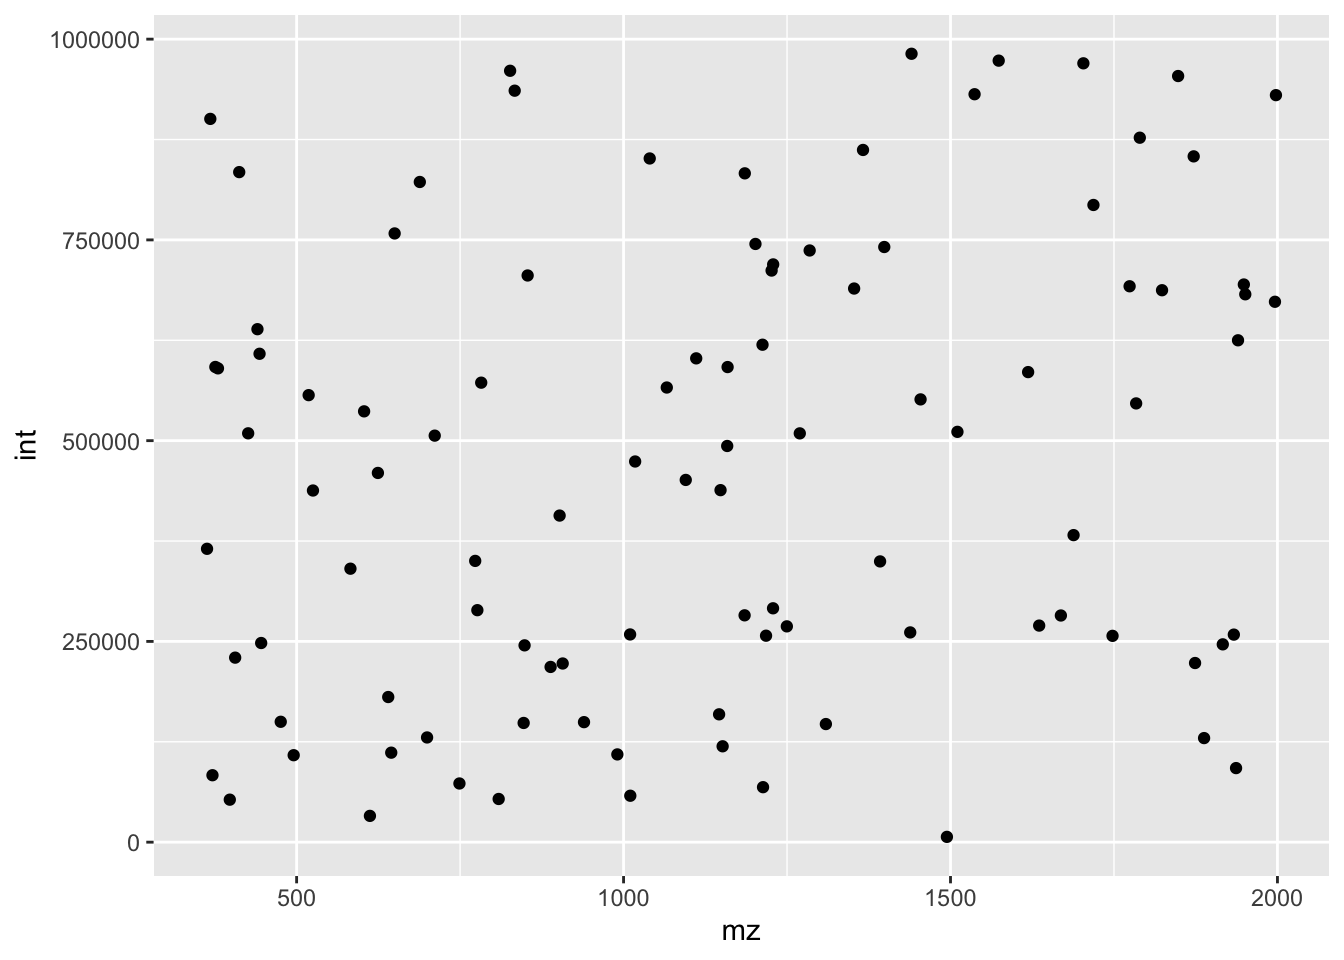
\includegraphics{_main_files/figure-latex/unnamed-chunk-66-1} \end{center}

In data analysis, creating a plot to convey a message or demonstrate a result is a common endpoint. To achieve this, this book utilizes the \texttt{GGPlot2} package, which is part of the \texttt{Tidyverse}. This package complements the data pipelining demonstrated in the previous chapters, making it a perfect choice for creating a wide range of plots, from simple scatter plots to complex heat maps, making it ideal for data visualization.

\hypertarget{base-plot}{%
\section{Base: plot}\label{base-plot}}

R comes standard with the fairly basic plotting function \texttt{plot()}. While this function forms the basis for all plotting interactions in R, it can be greatly extended with additional packages. Two such packages will be explored in this chapter, \texttt{GGplot2} and \texttt{Plotly}. The former is great for static publication quality plots, of which you will begin to recognize, while the latter provides stunning interactive graphics suitable for web development and Shiny applications.

\begin{Shaded}
\begin{Highlighting}[]
\FunctionTok{set.seed}\NormalTok{(}\DecValTok{1234}\NormalTok{)}
\FunctionTok{plot}\NormalTok{(}\FunctionTok{sample}\NormalTok{(}\DecValTok{1}\SpecialCharTok{:}\DecValTok{20}\NormalTok{),}\FunctionTok{sample}\NormalTok{(}\DecValTok{1}\SpecialCharTok{:}\DecValTok{20}\NormalTok{))}
\end{Highlighting}
\end{Shaded}

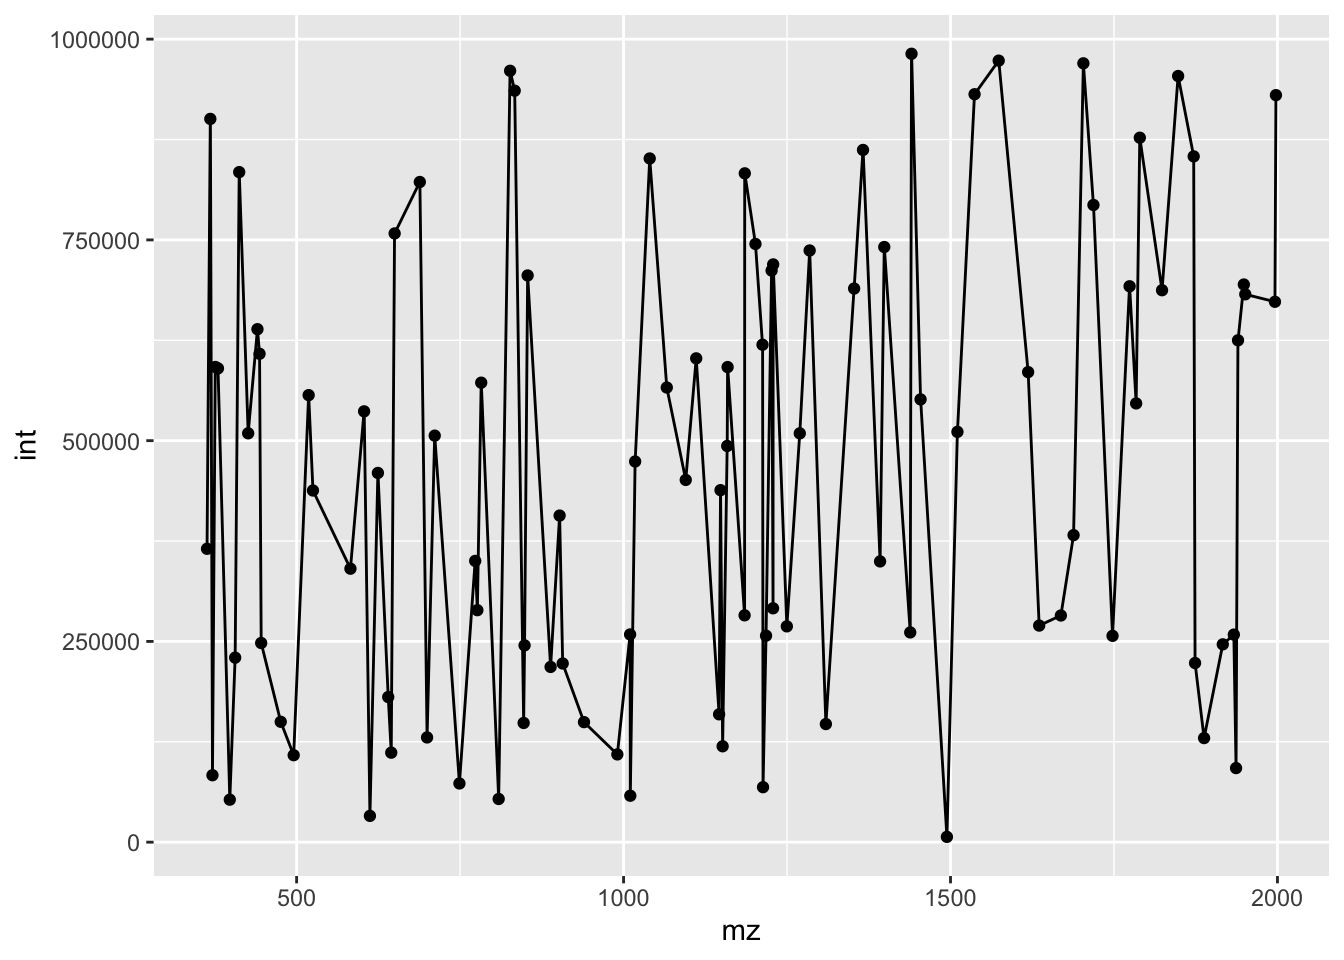
\includegraphics{_main_files/figure-latex/unnamed-chunk-67-1.pdf}

\begin{Shaded}
\begin{Highlighting}[]
\FunctionTok{set.seed}\NormalTok{(}\DecValTok{1234}\NormalTok{)}
\NormalTok{df }\OtherTok{\textless{}{-}} \FunctionTok{data.frame}\NormalTok{( }\AttributeTok{x1 =} \FunctionTok{sample}\NormalTok{(}\DecValTok{1}\SpecialCharTok{:}\DecValTok{20}\NormalTok{), }\AttributeTok{y1 =} \FunctionTok{sample}\NormalTok{(}\DecValTok{1}\SpecialCharTok{:}\DecValTok{20}\NormalTok{) )}
\NormalTok{df }\SpecialCharTok{\%\textgreater{}\%} \FunctionTok{plot}\NormalTok{()}
\end{Highlighting}
\end{Shaded}

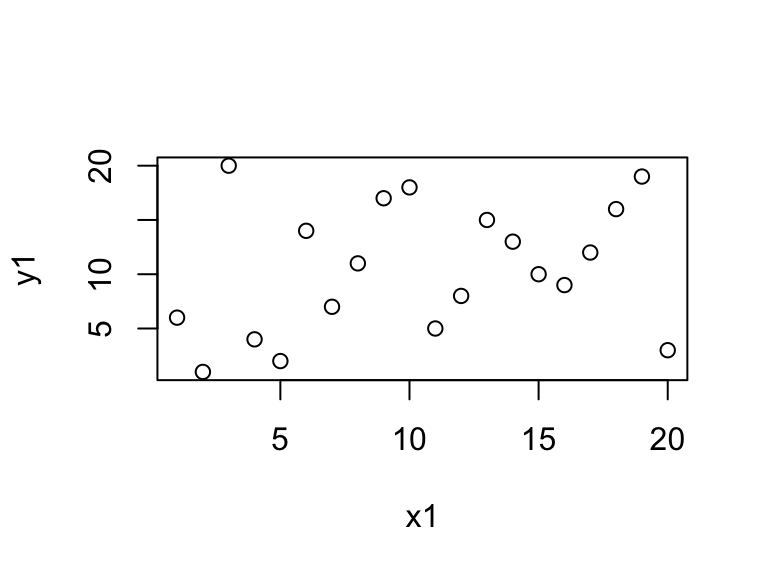
\includegraphics{_main_files/figure-latex/unnamed-chunk-68-1.pdf}

\hypertarget{ggplot}{%
\section{GGPlot}\label{ggplot}}

\begin{Shaded}
\begin{Highlighting}[]
\FunctionTok{library}\NormalTok{(tidyverse)}
\end{Highlighting}
\end{Shaded}

\hypertarget{syntax-1}{%
\subsection{Syntax}\label{syntax-1}}

The motivation behind GGplot is based on the grammar of graphics such that

\begin{quote}
\emph{``the idea that you can build every graph from the same few components''}
\end{quote}

Ideally this accomplishes dual goals of allowing you to quickly construct plots for initial analyses and checking for oddities (as explained above) and following the logical process of the plot construction.

To graph in GGPlot there are a few core embodiments that need to be considered.

\begin{longtable}[]{@{}
  >{\raggedright\arraybackslash}p{(\columnwidth - 4\tabcolsep) * \real{0.2500}}
  >{\raggedright\arraybackslash}p{(\columnwidth - 4\tabcolsep) * \real{0.3750}}
  >{\raggedright\arraybackslash}p{(\columnwidth - 4\tabcolsep) * \real{0.3750}}@{}}
\toprule\noalign{}
\endhead
\bottomrule\noalign{}
\endlastfoot
data & a table of numeric and/or categorical values & data.frame or tibble \\
geom & a geometric object or visual representation, that can be layered & points, lines, bars, boxs, etc. \\
aesthetics & how variables in the data are mapped to visual properties & eg. \emph{x = col\_a, y = col\_b} \\
coordinate & orientation of the data points & eg. \emph{cartesian (x,y), polar} \\
\end{longtable}

\begin{Shaded}
\begin{Highlighting}[]
\CommentTok{\# the basic structure}
\FunctionTok{ggplot}\NormalTok{(data, }\FunctionTok{aes}\NormalTok{(x,y)) }\SpecialCharTok{+} \FunctionTok{geom\_point}\NormalTok{() }\SpecialCharTok{+} \FunctionTok{coord\_cartiesian}\NormalTok{()}

\CommentTok{\# combined with dplyr makes for a readable process}
\NormalTok{data }\SpecialCharTok{\%\textgreater{}\%} \FunctionTok{ggplot}\NormalTok{(}\FunctionTok{aes}\NormalTok{(x,y)) }\SpecialCharTok{+} \FunctionTok{geom\_point}\NormalTok{()}
\end{Highlighting}
\end{Shaded}

In this example the \texttt{ggplot()} function contains the two components, the data table \texttt{data} and mapping function \texttt{aes()}. Since \emph{GGPlot} follows a layered modality, the \texttt{ggplot()} function ``sets'' the canvas and passes the data table \texttt{data} and mapping function \texttt{aes()} to all the functions that follow with the \texttt{+} operator.

Lets create some data \ldots{}

\begin{Shaded}
\begin{Highlighting}[]
\FunctionTok{set.seed}\NormalTok{(}\DecValTok{5}\NormalTok{)}
\NormalTok{tbl\_mz }\OtherTok{\textless{}{-}} \FunctionTok{tibble}\NormalTok{(}
  \AttributeTok{mz =} \FunctionTok{sample}\NormalTok{(}\DecValTok{3500}\SpecialCharTok{:}\DecValTok{20000}\SpecialCharTok{/}\DecValTok{10}\NormalTok{, }\DecValTok{100}\NormalTok{),}
  \AttributeTok{int =} \FunctionTok{rlnorm}\NormalTok{(}\AttributeTok{meanlog =} \DecValTok{5}\NormalTok{, }\AttributeTok{sdlog =} \DecValTok{2}\NormalTok{, }\DecValTok{100}\NormalTok{),}
  \AttributeTok{class =} \FunctionTok{sample}\NormalTok{(}\FunctionTok{c}\NormalTok{(}\StringTok{\textquotesingle{}A\textquotesingle{}}\NormalTok{,}\StringTok{\textquotesingle{}B\textquotesingle{}}\NormalTok{,}\StringTok{\textquotesingle{}C\textquotesingle{}}\NormalTok{,}\StringTok{\textquotesingle{}D\textquotesingle{}}\NormalTok{), }\DecValTok{100}\NormalTok{, }\AttributeTok{replace =} \ConstantTok{TRUE}\NormalTok{) }
\NormalTok{)}
\end{Highlighting}
\end{Shaded}

\hypertarget{basic-data-plotting}{%
\subsection{Basic Data Plotting}\label{basic-data-plotting}}

\hypertarget{points-and-lines}{%
\subsubsection*{Points and Lines}\label{points-and-lines}}
\addcontentsline{toc}{subsubsection}{Points and Lines}

Points and lines graphing is a simple way of representing data in a two-dimensional space. In this graph, we use points to represent individual data values, and lines to connect them. The x-axis usually represents the \textbf{independent} variable while the y-axis represents the \textbf{dependent} variable - or in other words, what \emph{y} was observed while measuring \emph{x}.

To plot a point, we use an ordered pair of values (x, y) that correspond to the position of the point on the graph. For example, the point (2, 5) would be plotted 2 units to the right on the x-axis and 5 units up on the y-axis.

We can also connect points with lines to show a trend or pattern in the data. These lines can be straight or curved, depending on the nature of the data. A straight line can be drawn to connect two points or to represent a linear relationship between the variables.

\begin{Shaded}
\begin{Highlighting}[]
\NormalTok{p01 }\OtherTok{\textless{}{-}}\NormalTok{ tbl\_mz }\SpecialCharTok{\%\textgreater{}\%} \FunctionTok{ggplot}\NormalTok{(}\FunctionTok{aes}\NormalTok{(mz, int)) }\SpecialCharTok{+} \FunctionTok{geom\_point}\NormalTok{()}
\NormalTok{p02 }\OtherTok{\textless{}{-}}\NormalTok{ tbl\_mz }\SpecialCharTok{\%\textgreater{}\%} \FunctionTok{ggplot}\NormalTok{(}\FunctionTok{aes}\NormalTok{(mz, int)) }\SpecialCharTok{+} \FunctionTok{geom\_line}\NormalTok{()}
\NormalTok{p03 }\OtherTok{\textless{}{-}}\NormalTok{ tbl\_mz }\SpecialCharTok{\%\textgreater{}\%} \FunctionTok{ggplot}\NormalTok{(}\FunctionTok{aes}\NormalTok{(mz, int)) }\SpecialCharTok{+} \FunctionTok{geom\_point}\NormalTok{(}\AttributeTok{color=}\StringTok{\textquotesingle{}red\textquotesingle{}}\NormalTok{) }\SpecialCharTok{+} \FunctionTok{geom\_line}\NormalTok{(}\AttributeTok{color=}\StringTok{\textquotesingle{}black\textquotesingle{}}\NormalTok{)}
\NormalTok{p04 }\OtherTok{\textless{}{-}}\NormalTok{ tbl\_mz }\SpecialCharTok{\%\textgreater{}\%} \FunctionTok{ggplot}\NormalTok{(}\FunctionTok{aes}\NormalTok{(mz, int)) }\SpecialCharTok{+} \FunctionTok{geom\_line}\NormalTok{(}\AttributeTok{color=}\StringTok{\textquotesingle{}black\textquotesingle{}}\NormalTok{) }\SpecialCharTok{+} \FunctionTok{geom\_point}\NormalTok{(}\AttributeTok{color=}\StringTok{\textquotesingle{}red\textquotesingle{}}\NormalTok{)}
\end{Highlighting}
\end{Shaded}

It's important to take note of the difference between plots \emph{p03} and \emph{p04}. While both plots showcase a similar data representation, a closer look reveals a notable difference. Specifically, in the latter plot (\emph{p04}), we can see that the red points appear under the black line. This occurs because the points were layered first, and then the lines were layered over them. This is a crucial distinction to make as it highlights the importance of the order in which layers are applied in the plot.
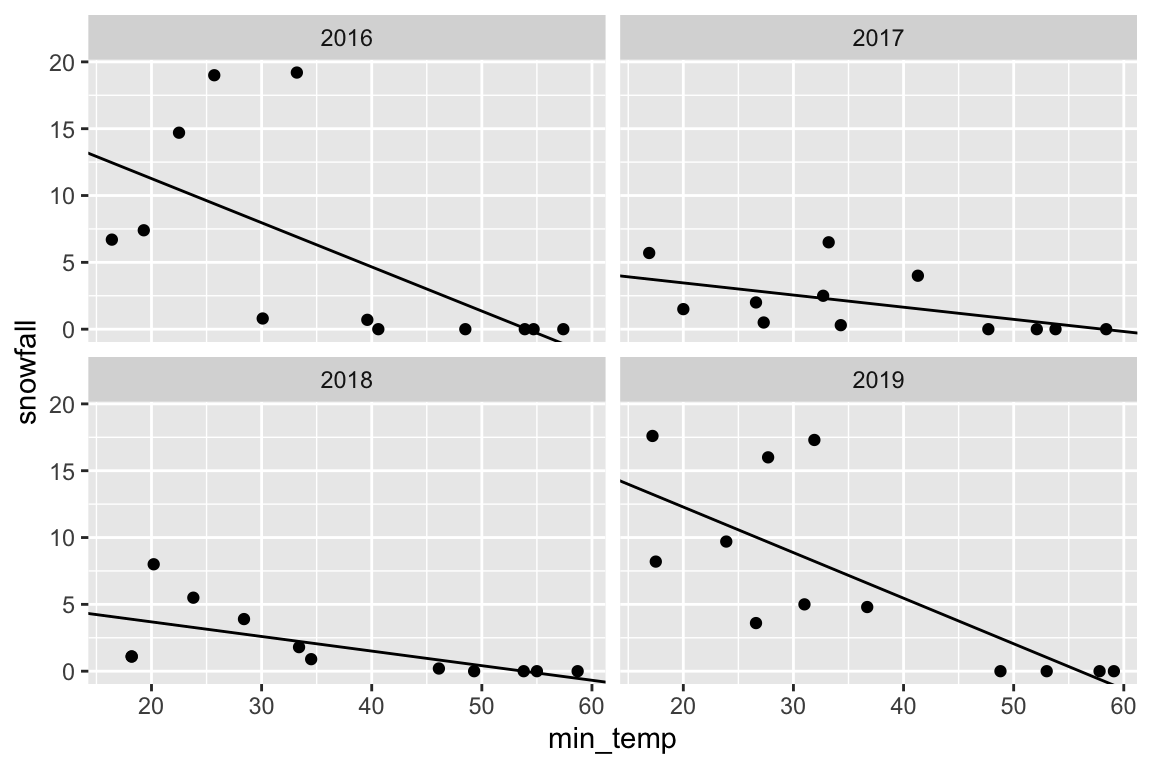
\includegraphics{_main_files/figure-latex/unnamed-chunk-74-1.pdf}

\hypertarget{segments}{%
\subsubsection*{Segments}\label{segments}}
\addcontentsline{toc}{subsubsection}{Segments}

Line segments are an important concept in geometry and are used in various applications. A line segment is a part of a line that is bounded by two distinct end points. It is also a default representation of centroided mass spectra. In this case the segment will start and end on the same \emph{x} (mz), while the \emph{y} (int) component will end at 0.

\begin{Shaded}
\begin{Highlighting}[]
\NormalTok{p05 }\OtherTok{\textless{}{-}}\NormalTok{ tbl\_mz }\SpecialCharTok{\%\textgreater{}\%} \FunctionTok{ggplot}\NormalTok{(}\FunctionTok{aes}\NormalTok{(mz, int)) }\SpecialCharTok{+} \FunctionTok{geom\_segment}\NormalTok{(}\FunctionTok{aes}\NormalTok{(}\AttributeTok{xend =}\NormalTok{ mz, }\AttributeTok{yend =} \DecValTok{0}\NormalTok{))}
\end{Highlighting}
\end{Shaded}

\begin{center}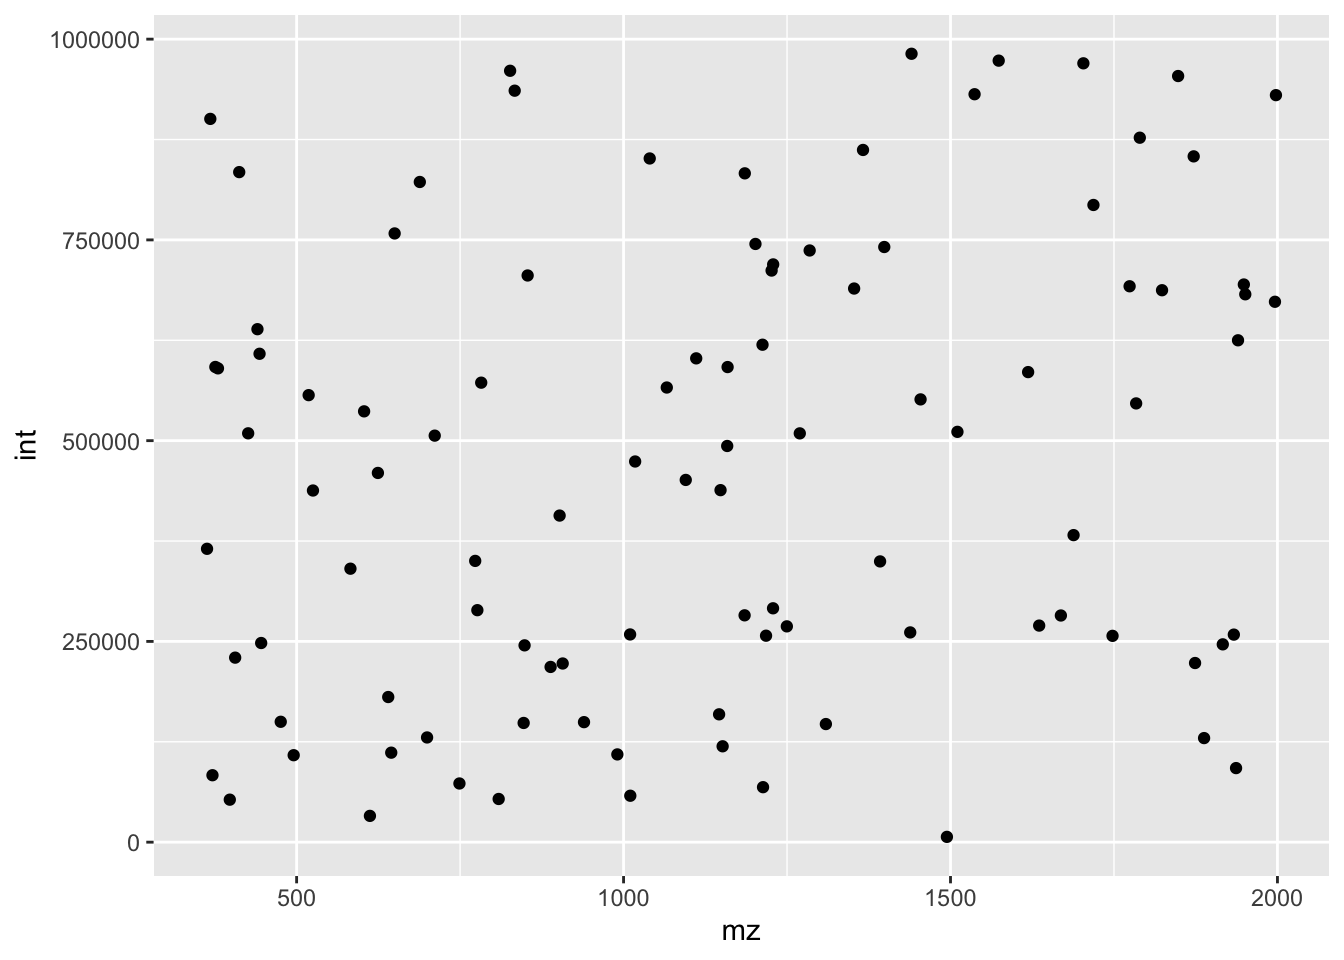
\includegraphics{_main_files/figure-latex/unnamed-chunk-76-1} \end{center}

\hypertarget{bar-chart}{%
\subsubsection*{Bar Chart}\label{bar-chart}}
\addcontentsline{toc}{subsubsection}{Bar Chart}

When it comes to representing categorical data, bar charts are considered to be the most effective visualization tool. Bar charts are simple, yet powerful, and can be used to display data in a clear and concise way. They are easy to read and understand, and are a popular choice among data analysts, researchers, and business professionals. Whether you're trying to visualize sales data, survey results, or demographic information, bar charts are a great option to consider. So, if you're looking for a way to represent categorical data, consider using a bar chart for the most accurate and comprehensive representation.

\begin{Shaded}
\begin{Highlighting}[]
\NormalTok{p06 }\OtherTok{\textless{}{-}}\NormalTok{ tbl\_mz }\SpecialCharTok{\%\textgreater{}\%} \FunctionTok{ggplot}\NormalTok{(}\FunctionTok{aes}\NormalTok{(class)) }\SpecialCharTok{+} \FunctionTok{geom\_bar}\NormalTok{()}
\end{Highlighting}
\end{Shaded}

\begin{center}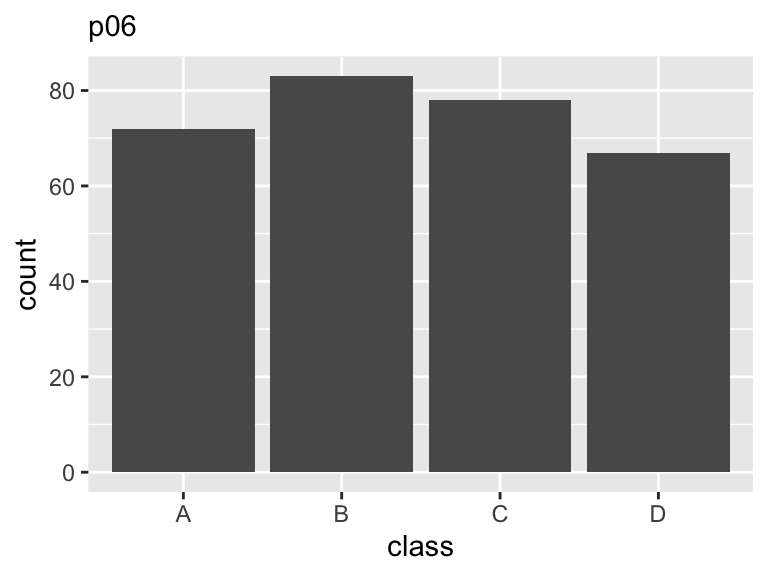
\includegraphics{_main_files/figure-latex/unnamed-chunk-78-1} \end{center}

\hypertarget{pie-chart}{%
\subsubsection*{Pie Chart}\label{pie-chart}}
\addcontentsline{toc}{subsubsection}{Pie Chart}

You maybe considering a pie chart, which is a circular diagram divided into sectors, with each sector representing a proportion of the whole. It is commonly used to display percentages, where the sum of the sectors equals 100\%. There is no specific \texttt{geom} to build piechart with ggplot2. The trick is to build a barplot and use \texttt{coord\_polar()} to make it circular. However, interpreting pie charts can be challenging since humans are not very skilled at reading angles. For instance, it is often difficult to determine which group is the largest and to arrange them by value. As a result, it is advisable to refrain from using pie charts.

\begin{Shaded}
\begin{Highlighting}[]
\NormalTok{p07 }\OtherTok{\textless{}{-}}\NormalTok{ tbl\_mz }\SpecialCharTok{\%\textgreater{}\%} \FunctionTok{ggplot}\NormalTok{(}\FunctionTok{aes}\NormalTok{(class, }\AttributeTok{fill=}\NormalTok{class)) }\SpecialCharTok{+} \FunctionTok{geom\_bar}\NormalTok{()}
\NormalTok{p08 }\OtherTok{\textless{}{-}}\NormalTok{ tbl\_mz }\SpecialCharTok{\%\textgreater{}\%} \FunctionTok{ggplot}\NormalTok{(}\FunctionTok{aes}\NormalTok{(class, }\AttributeTok{fill=}\NormalTok{class)) }\SpecialCharTok{+} \FunctionTok{geom\_bar}\NormalTok{() }\SpecialCharTok{+} \FunctionTok{coord\_flip}\NormalTok{()}
\NormalTok{p09 }\OtherTok{\textless{}{-}}\NormalTok{ tbl\_mz }\SpecialCharTok{\%\textgreater{}\%} \FunctionTok{ggplot}\NormalTok{(}\FunctionTok{aes}\NormalTok{(}\DecValTok{1}\NormalTok{, }\AttributeTok{fill=}\NormalTok{class)) }\SpecialCharTok{+} \FunctionTok{geom\_bar}\NormalTok{(}\AttributeTok{position =} \StringTok{\textquotesingle{}fill\textquotesingle{}}\NormalTok{) }\SpecialCharTok{+} \FunctionTok{coord\_polar}\NormalTok{(}\AttributeTok{theta =} \StringTok{\textquotesingle{}y\textquotesingle{}}\NormalTok{)}
\end{Highlighting}
\end{Shaded}

\begin{center}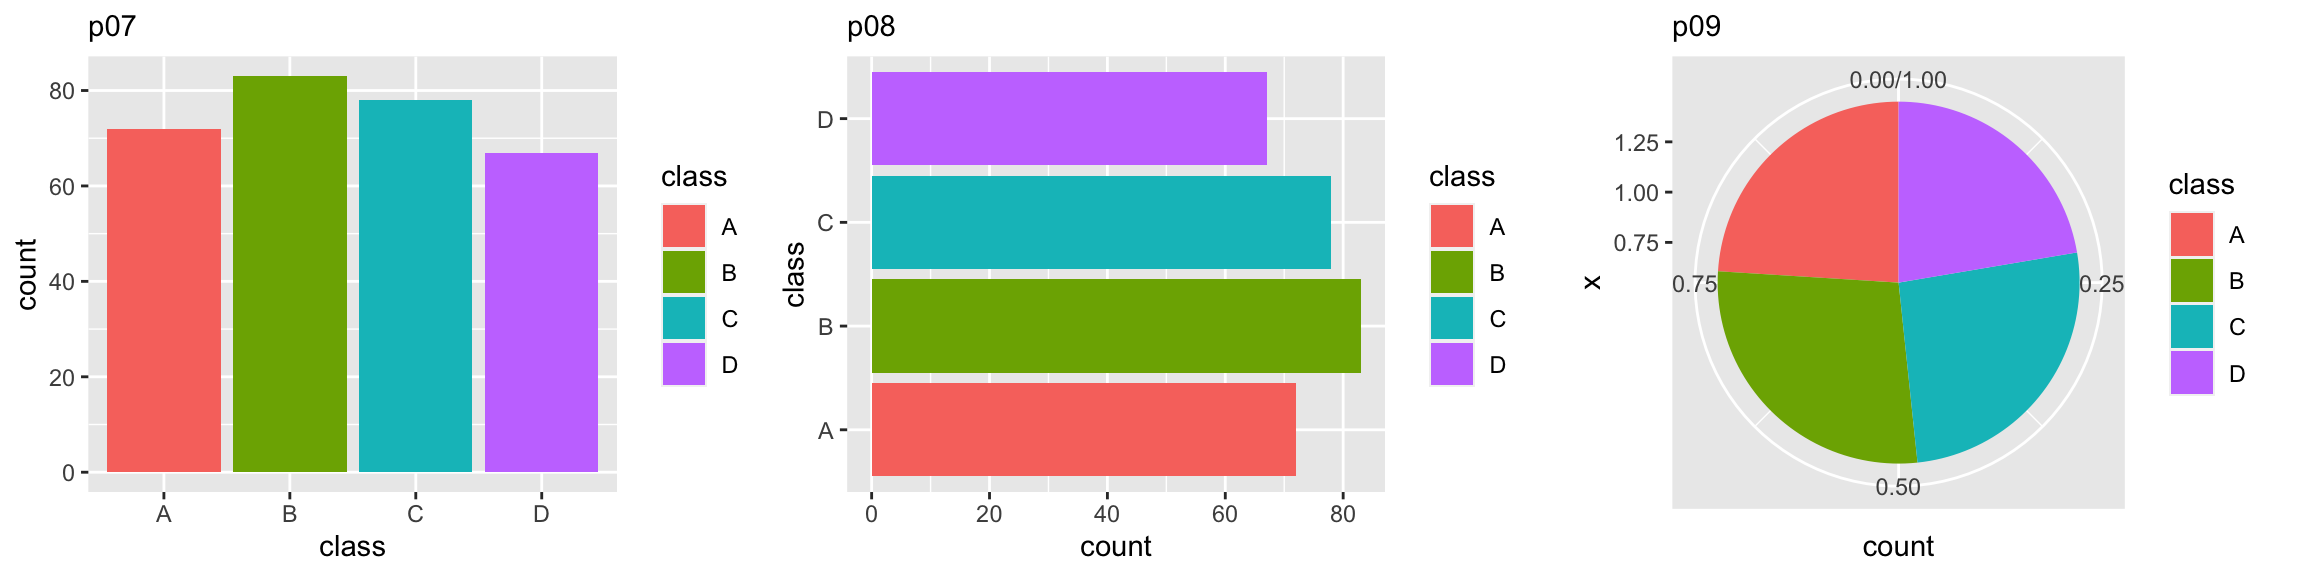
\includegraphics{_main_files/figure-latex/unnamed-chunk-80-1} \end{center}

Note how difficult it is in the pie chart to tell (by eye) that \emph{A} is the smallest.

\hypertarget{data-distributions}{%
\subsection{Data Distributions}\label{data-distributions}}

In statistics, a distribution refers to the way in which a set of data is spread out or dispersed. It describes the pattern of values that a variable can take and how frequently each value occurs. A distribution can be characterized by its shape, center, and spread, and can be represented graphically using tools such as histograms, box plots, and density plots.

\hypertarget{histograms}{%
\subsubsection*{Histograms}\label{histograms}}
\addcontentsline{toc}{subsubsection}{Histograms}

A histogram is a graphical representation of the distribution of a dataset. It is a type of bar chart that displays the frequency of data values falling into specified intervals or ranges of values, known as bins. The x-axis of the histogram represents the bins or intervals, and the y-axis represents the frequency or count of values falling into each bin.

Histograms are widely used to summarize large datasets and identify patterns or trends and to visualize the shape of a distribution, whether it is symmetric or skewed, and whether it has any outliers or gaps in the data. They can also be used to compare the distributions of two or more datasets, by plotting them on the same graph with different colors or patterns.

\begin{Shaded}
\begin{Highlighting}[]
\NormalTok{p10 }\OtherTok{\textless{}{-}}\NormalTok{ tbl\_mz }\SpecialCharTok{\%\textgreater{}\%} \FunctionTok{ggplot}\NormalTok{(}\FunctionTok{aes}\NormalTok{(}\FunctionTok{log}\NormalTok{(int))) }\SpecialCharTok{+} \FunctionTok{geom\_histogram}\NormalTok{(}\AttributeTok{binwidth =} \DecValTok{1}\NormalTok{)}
\end{Highlighting}
\end{Shaded}

\begin{center}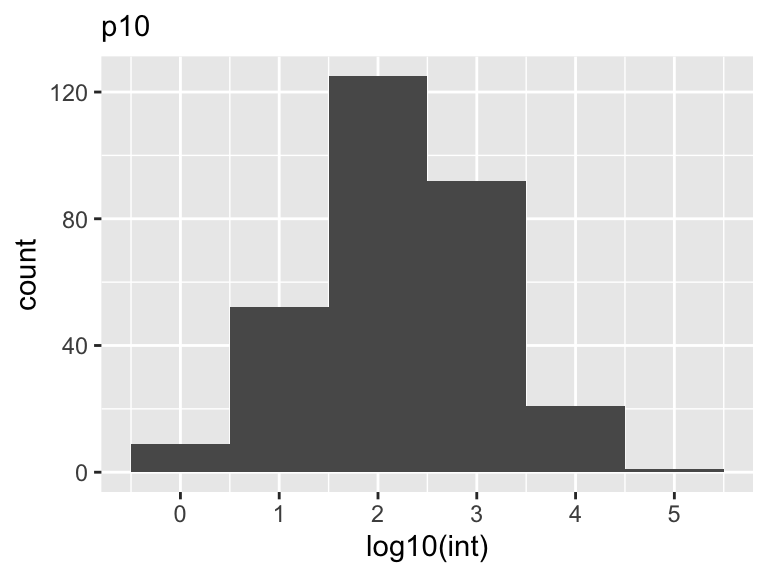
\includegraphics{_main_files/figure-latex/unnamed-chunk-82-1} \end{center}

\hypertarget{density}{%
\subsubsection*{Density}\label{density}}
\addcontentsline{toc}{subsubsection}{Density}

A density plot is a graphical representation of the distribution of a dataset. It is formed by smoothing the data values and representing them as a continuous probability density function. The density plot is a variation of the histogram that provides a smoother representation of the data, eliminating the need for binning. It is particularly useful when the data is continuous and the sample size is large. The density plot can be used to identify the shape of the distribution, the presence of multiple modes, and the presence of outliers. Again, it can also be used to compare the distributions of two or more datasets by overlaying them on the same plot.

\begin{Shaded}
\begin{Highlighting}[]
\NormalTok{p11 }\OtherTok{\textless{}{-}}\NormalTok{ tbl\_mz }\SpecialCharTok{\%\textgreater{}\%} \FunctionTok{ggplot}\NormalTok{(}\FunctionTok{aes}\NormalTok{(}\FunctionTok{log}\NormalTok{(int))) }\SpecialCharTok{+} \FunctionTok{geom\_density}\NormalTok{()}
\end{Highlighting}
\end{Shaded}

\begin{center}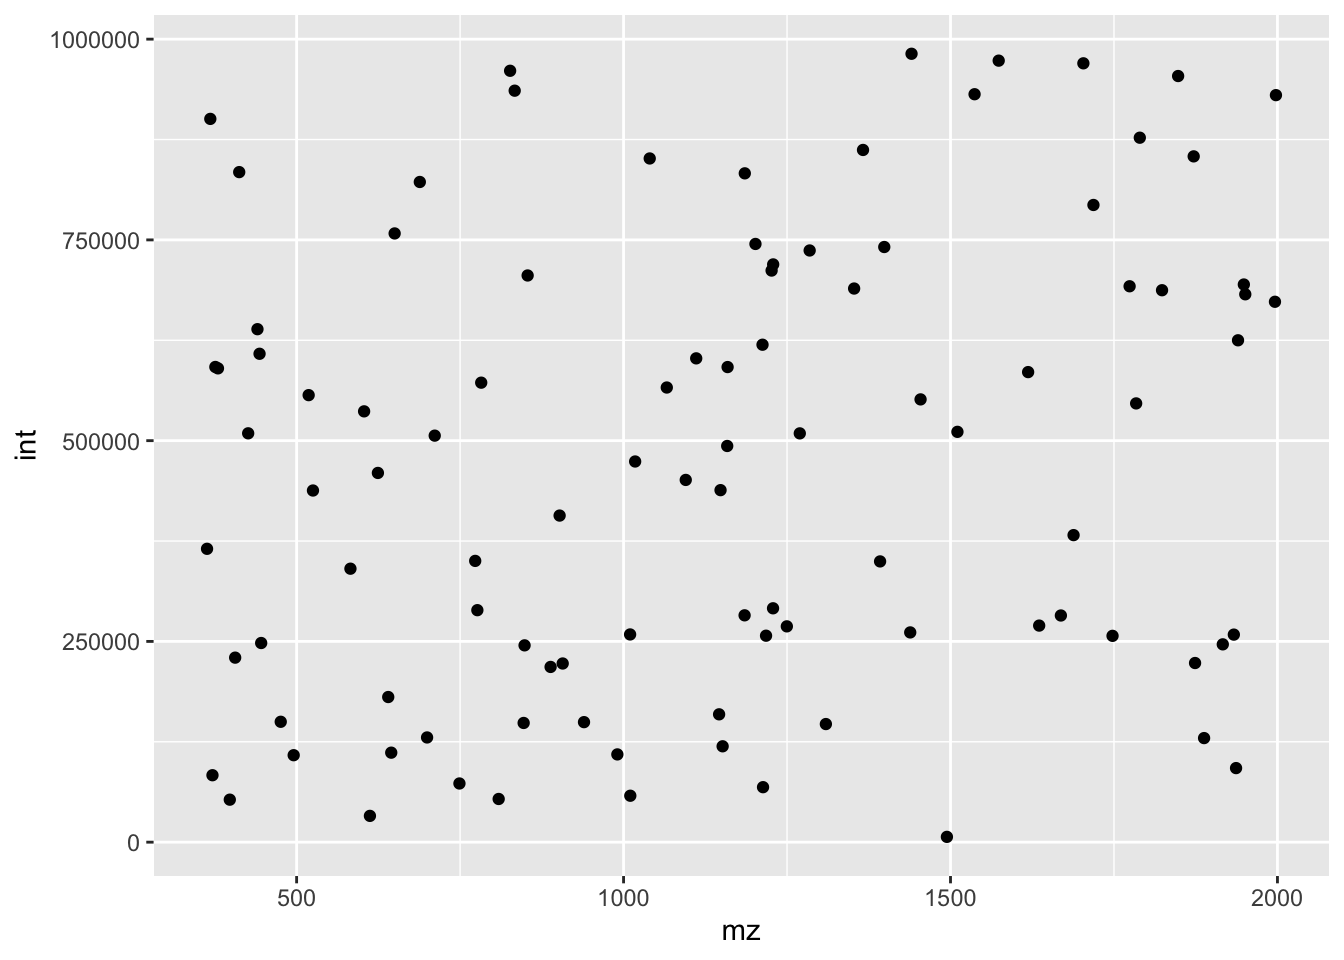
\includegraphics{_main_files/figure-latex/unnamed-chunk-84-1} \end{center}

\hypertarget{extended-syntax}{%
\subsection{Extended Syntax}\label{extended-syntax}}

\hypertarget{colors}{%
\subsubsection{Colors}\label{colors}}

\hypertarget{scales}{%
\subsubsection{Scales}\label{scales}}

\hypertarget{faceting}{%
\subsubsection{Faceting}\label{faceting}}

\hypertarget{labels}{%
\subsubsection{Labels}\label{labels}}

\hypertarget{annotations}{%
\subsubsection{Annotations}\label{annotations}}

\hypertarget{package-ggrepel}{%
\subsubsection{Package ggrepel}\label{package-ggrepel}}

\hypertarget{plotly}{%
\section{Plotly}\label{plotly}}

\hypertarget{mass-spectrometry-data}{%
\chapter{Mass Spectrometry Data}\label{mass-spectrometry-data}}

\hypertarget{commercial}{%
\section{Commercial}\label{commercial}}

\hypertarget{raw-thermo}{%
\subsection{RAW (Thermo)}\label{raw-thermo}}

\hypertarget{wiff-sciex}{%
\subsection{WIFF (Sciex)}\label{wiff-sciex}}

\hypertarget{d-agilent}{%
\subsection{D (Agilent)}\label{d-agilent}}

\hypertarget{d-bruker}{%
\subsection{D (Bruker)}\label{d-bruker}}

\hypertarget{open-access-raw-data}{%
\section{Open Access Raw Data}\label{open-access-raw-data}}

Mass spectrometry (MS) is a powerful analytical method that can be used to determine the mass-to-charge ratio (m/z) of ions in a sample. Mass spectrometry data is generated from MS experiments and can be stored in various formats, including mzXML, mzML, and mzH5.

\hypertarget{conversion-tools}{%
\subsection*{Conversion Tools}\label{conversion-tools}}
\addcontentsline{toc}{subsection}{Conversion Tools}

ProteoWizard is an open-source software tool that provides a collection of open-source, cross-platform software libraries and tools for extracting raw mass spectrometry data from from various instrument vendor formats and converting it to the formats listed below.

\begin{quote}
\emph{Kessner, D., Chambers, M., Burke, R., Agus, D., \& Mallick, P. (2008). ProteoWizard: open source software for rapid proteomics tools development. Bioinformatics, 24(21), 2534--2536. \url{https://doi.org/10.1093/bioinformatics/btn323}}

\url{https://proteowizard.sourceforge.io/}
\end{quote}

\hypertarget{mzxml}{%
\subsection*{mzXML}\label{mzxml}}
\addcontentsline{toc}{subsection}{mzXML}

mzXML is an open XML-based format for encoding MS data. It was developed by the Seattle Proteome Center and is widely used in the mass spectrometry community. mzXML files contain raw MS data, as well as metadata describing the instrument parameters used to acquire the data. mzXML files can be processed using a variety of software tools, such as the Trans-Proteomic Pipeline and ProteoWizard.

The mzXML format has been shown to be effective in handling data from a wide range of instruments. It has a simple structure that makes it easy to parse and process, making it an attractive choice for many researchers. The format is also relatively lightweight, which makes it easy to transfer and store large amounts of data.

\begin{quote}
\emph{Pedrioli, P.G., Eng, J.K., Hubley, R., Vogelzang, M., Deutsch, E.W., Raught, B., Pratt, B., Nilsson, E., Angeletti, R.H., Apweiler, R. and Cheung, K., 2004. A common open representation of mass spectrometry data and its application to proteomics research. Nature biotechnology, 22(11), pp.1459-1466.}
\end{quote}

\hypertarget{mzml}{%
\subsection*{mzML}\label{mzml}}
\addcontentsline{toc}{subsection}{mzML}

The mzML format is another open XML-based format for MS data, developed by the Proteomics Standards Initiative. It is designed to be more flexible than mzXML and includes more detailed metadata. mzML files can be processed using software tools such as OpenMS and mzR.

The mzML format allows for more detailed and comprehensive data storage than mzXML. This is because mzML has a more complex structure, which enables the storage of a wider range of experimental metadata. The format is also more flexible, which means that it can be easily adapted to different types of experiments and instruments.

\begin{quote}
\emph{Martens, L., Chambers, M., Sturm, M., Kessner, D., Levander, F., Shofstahl, J., Tang, W.H., Römpp, A., Neumann, S., Pizarro, A.D. and Montecchi-Palazzi, L., 2011. mzML---a community standard for mass spectrometry data. Molecular \& cellular proteomics, 10(1), p.R110. 000133.}
\end{quote}

\hypertarget{mzmlb}{%
\subsection*{mzMLb}\label{mzmlb}}
\addcontentsline{toc}{subsection}{mzMLb}

Recently proposed as a new file format based on HDF5 and NetCDF4 standards, mzMLb is faster and more flexible than existing approaches while preserving the XML encoding of metadata. Additionally, it is optimized for both read/write speed and storage efficiency. The format has a reference implementation provided within the ProteoWizard toolkit.

\begin{quote}
Bhamber, Ranjeet S., et al.~``mzMLb: A future-proof raw mass spectrometry data format based on standards-compliant mzML and optimized for speed and storage requirements.'' Journal of proteome research 20.1 (2020): 172-183.\_
\end{quote}

\hypertarget{mass-spectrometry-r-packages-work-in-progress}{%
\chapter{Mass Spectrometry R Packages (work in progress)}\label{mass-spectrometry-r-packages-work-in-progress}}

\hypertarget{xcms}{%
\section{xcms}\label{xcms}}

\hypertarget{deqms}{%
\section{deqms}\label{deqms}}

\hypertarget{msempire}{%
\section{msempire}\label{msempire}}

\hypertarget{msqrob}{%
\section{msqrob}\label{msqrob}}

\hypertarget{msstatstmt}{%
\section{MSstatsTMT}\label{msstatstmt}}

\hypertarget{msstats}{%
\section{MSstats}\label{msstats}}

The MSstats package is an R package designed for the analysis of label-free mass spectrometry data. It provides a wide range of statistical tools for the analysis of protein abundance data, including normalization, missing value imputation, quality control, and differential expression analysis. MSstats provides a powerful and flexible way to analyze mass spectrometry data, making it an essential tool for researchers in the field.

\begin{longtable}[]{@{}
  >{\raggedright\arraybackslash}p{(\columnwidth - 2\tabcolsep) * \real{0.2222}}
  >{\raggedright\arraybackslash}p{(\columnwidth - 2\tabcolsep) * \real{0.7778}}@{}}
\toprule\noalign{}
\endhead
\bottomrule\noalign{}
\endlastfoot
\textbf{Documentation} & \href{https://msstats.org}{web}, \href{https://bioconductor.org/packages/release/bioc/manuals/MSstats/man/MSstats.pdf}{PDF} \\
\textbf{Code} & \href{https://www.bioconductor.org/packages/release/bioc/html/MSstats.html}{Bioconductor} \\
\textbf{Literature} & \emph{Bioinformatics} 30.17 (2014): 2524-2526 \\
\end{longtable}

\hypertarget{installation-1}{%
\subsection{Installation}\label{installation-1}}

To install MSstats, you can use the following code:

\begin{Shaded}
\begin{Highlighting}[]
\ControlFlowTok{if}\NormalTok{ (}\SpecialCharTok{!}\FunctionTok{requireNamespace}\NormalTok{(}\StringTok{"BiocManager"}\NormalTok{, }\AttributeTok{quietly =} \ConstantTok{TRUE}\NormalTok{))}
    \FunctionTok{install.packages}\NormalTok{(}\StringTok{"BiocManager"}\NormalTok{)}

\NormalTok{BiocManager}\SpecialCharTok{::}\FunctionTok{install}\NormalTok{(}\StringTok{"MSstats"}\NormalTok{)}
\end{Highlighting}
\end{Shaded}

\hypertarget{loading-data}{%
\subsection{Loading Data}\label{loading-data}}

To load your data into MSstats, you can use the following code:

\begin{Shaded}
\begin{Highlighting}[]
\FunctionTok{library}\NormalTok{(MSstats)}
\FunctionTok{data}\NormalTok{(}\StringTok{"QCMAPData"}\NormalTok{)}
\NormalTok{data }\OtherTok{\textless{}{-}}\NormalTok{ QCMAPData}\SpecialCharTok{$}\NormalTok{data}
\NormalTok{design }\OtherTok{\textless{}{-}}\NormalTok{ QCMAPData}\SpecialCharTok{$}\NormalTok{design}
\FunctionTok{head}\NormalTok{(data)}
\end{Highlighting}
\end{Shaded}

\hypertarget{quality-control}{%
\subsection{Quality Control}\label{quality-control}}

To perform quality control on your data, you can use the following code:

\begin{Shaded}
\begin{Highlighting}[]
\NormalTok{QCmetrics }\OtherTok{\textless{}{-}}\NormalTok{ MSstats}\SpecialCharTok{:::}\FunctionTok{calculateQCmetrics}\NormalTok{(data, }\AttributeTok{featureLevel =} \StringTok{"protein"}\NormalTok{)}
\NormalTok{MSstats}\SpecialCharTok{:::}\FunctionTok{plotQCmetrics}\NormalTok{(QCmetrics, }\AttributeTok{plotType =} \StringTok{"boxplot"}\NormalTok{,}
                        \AttributeTok{ylim =} \FunctionTok{c}\NormalTok{(}\DecValTok{0}\NormalTok{, }\DecValTok{200000}\NormalTok{), }\AttributeTok{ylab =} \StringTok{"Total Ion Current"}\NormalTok{)}
\end{Highlighting}
\end{Shaded}

\hypertarget{differential-expression-analysis}{%
\subsection{Differential Expression Analysis}\label{differential-expression-analysis}}

To perform differential expression analysis on your data, you can use the following code:

\begin{Shaded}
\begin{Highlighting}[]
\NormalTok{MSstatsResult }\OtherTok{\textless{}{-}}\NormalTok{ MSstats}\SpecialCharTok{::}\FunctionTok{MSstats}\NormalTok{(data, design,}
                                  \AttributeTok{normalizationMethod =} \StringTok{"quantile"}\NormalTok{,}
                                  \AttributeTok{normalization =} \StringTok{"median"}\NormalTok{,}
                                  \AttributeTok{msLevel =} \DecValTok{1}\NormalTok{, }\AttributeTok{verbose =} \ConstantTok{TRUE}\NormalTok{)}
\FunctionTok{summary}\NormalTok{(MSstatsResult)}
\end{Highlighting}
\end{Shaded}

\hypertarget{conclusion}{%
\subsection{Conclusion}\label{conclusion}}

Overall, MSstats is a powerful and flexible R package for the analysis of label-free mass spectrometry data. It provides a wide range of statistical tools for the analysis of protein abundance data, making it an essential tool for researchers in the field. With its easy-to-use interface and comprehensive documentation, MSstats is a must-have tool for anyone working with mass spectrometry data.

\hypertarget{msgrob2}{%
\section{msgrob2}\label{msgrob2}}

\texttt{msgrob2} is an R package that provides functions to perform robust estimation in linear models with missing data. With the help of the Expectation-Maximization (EM) algorithm, the package estimates the parameters of the linear model and imputes the missing data. Additionally, the package offers robust methods for estimating the covariance matrix, including the Minimum Covariance Determinant (MCD) estimator and the S-estimator.

The \texttt{msgrob2} package is particularly useful in situations where data is missing from a linear model. The EM algorithm implemented in the package is a powerful tool for imputing missing data, and the robust covariance estimators allow for a better understanding of the data. The package is designed to provide efficient and accurate results when working with incomplete data, making it an essential tool for researchers and data analysts.

\begin{longtable}[]{@{}
  >{\raggedright\arraybackslash}p{(\columnwidth - 2\tabcolsep) * \real{0.2500}}
  >{\raggedright\arraybackslash}p{(\columnwidth - 2\tabcolsep) * \real{0.7500}}@{}}
\toprule\noalign{}
\endhead
\bottomrule\noalign{}
\endlastfoot
\textbf{Documentation} & \href{https://www.bioconductor.org/packages/release/bioc/manuals/msqrob2/man/msqrob2.pdf}{PDF} \\
\textbf{Code} & \href{https://www.bioconductor.org/packages/release/bioc/html/msqrob2.html}{Bioconductor} \\
\textbf{Literature} & \emph{Molecular \& Cellular Proteomics}, \textbf{15}(2), 657-668., \emph{Molecular \& Cellular Proteomics}, \textbf{19}(7), 1209-1219., \emph{Analytical Chemistry}, \textbf{92}(9), 6278--6287. \\
\end{longtable}

\hypertarget{code-examples}{%
\subsection{Code Examples}\label{code-examples}}

\hypertarget{installing-package}{%
\subsubsection{Installing Package}\label{installing-package}}

To install the \texttt{msgrob2} package, you can use the following code:

\begin{Shaded}
\begin{Highlighting}[]
\FunctionTok{install.packages}\NormalTok{(}\StringTok{"msgrob2"}\NormalTok{)}
\end{Highlighting}
\end{Shaded}

\hypertarget{loading-package}{%
\subsubsection{Loading Package}\label{loading-package}}

After installation, you can load the \texttt{msgrob2} package using the following code:

\begin{Shaded}
\begin{Highlighting}[]
\FunctionTok{library}\NormalTok{(msgrob2)}
\end{Highlighting}
\end{Shaded}

\hypertarget{estimating-parameters}{%
\subsubsection{Estimating Parameters}\label{estimating-parameters}}

To estimate the parameters of a linear model with missing data using \texttt{msgrob2}, you can use the \texttt{msgrob()} function. The following code demonstrates how to use \texttt{msgrob()}:

\begin{Shaded}
\begin{Highlighting}[]
\CommentTok{\# Loading Example Data}
\FunctionTok{data}\NormalTok{(}\StringTok{"exMiss"}\NormalTok{)}

\CommentTok{\# Estimating Parameters}
\NormalTok{model }\OtherTok{\textless{}{-}} \FunctionTok{lm}\NormalTok{(y }\SpecialCharTok{\textasciitilde{}}\NormalTok{ x1 }\SpecialCharTok{+}\NormalTok{ x2 }\SpecialCharTok{+}\NormalTok{ x3, }\AttributeTok{data =}\NormalTok{ exMiss)}
\FunctionTok{msgrob}\NormalTok{(model)}
\end{Highlighting}
\end{Shaded}

\hypertarget{estimating-covariance-matrix}{%
\subsubsection{Estimating Covariance Matrix}\label{estimating-covariance-matrix}}

To estimate the covariance matrix using \texttt{msgrob2}, you can use the \texttt{covrob()} function. The following code demonstrates how to use \texttt{covrob()}:

\begin{Shaded}
\begin{Highlighting}[]
\CommentTok{\# Loading Example Data}
\FunctionTok{data}\NormalTok{(}\StringTok{"exMiss"}\NormalTok{)}

\CommentTok{\# Estimating Covariance Matrix}
\FunctionTok{covrob}\NormalTok{(exMiss[,}\DecValTok{2}\SpecialCharTok{:}\DecValTok{4}\NormalTok{], }\AttributeTok{method =} \StringTok{"MCD"}\NormalTok{)}
\end{Highlighting}
\end{Shaded}

In summary, \texttt{msgrob2} is a comprehensive R package that provides an array of functions for robust estimation in linear models with missing data. The package's implementation of the EM algorithm and robust covariance estimators make it an essential tool for researchers and data analysts working with incomplete data. The package is easy to install and use, with code examples readily available for reference.

\hypertarget{statspro-r-package}{%
\section{StatsPro R Package}\label{statspro-r-package}}

\begin{longtable}[]{@{}
  >{\raggedright\arraybackslash}p{(\columnwidth - 2\tabcolsep) * \real{0.2222}}
  >{\raggedright\arraybackslash}p{(\columnwidth - 2\tabcolsep) * \real{0.7778}}@{}}
\toprule\noalign{}
\endhead
\bottomrule\noalign{}
\endlastfoot
\textbf{Documentation} & \href{https://github.com/YanglabWCH/StatsPro\#Readme}{github}, \href{https://github.com/YanglabWCH/StatsPro/blob/main/StatsPro_Manual.pdf}{PDF} \\
\textbf{Code} & \href{https://github.com/YanglabWCH/StatsPro}{github} \\
\textbf{Literature} & \emph{Journal of Proteomics} 250 (2022): 104386. \\
\end{longtable}

\hypertarget{tidyproteomics}{%
\section{Tidyproteomics}\label{tidyproteomics}}

The tidyproteomics R package is a tool that provides a set of functions to preprocess and analyze proteomics data using the tidy data framework. This package is built on top of the tidyverse and Bioconductor packages, which are widely used in the R community for data manipulation and analysis.

Some of the main features of the tidyproteomics package include:

\begin{itemize}
\tightlist
\item
  Data preprocessing functions for common tasks such as filtering, normalization, and imputation.
\item
  Functions for quality assessment and visualization of proteomics data.
\item
  Integration with other Bioconductor packages for downstream analysis such as differential expression analysis and pathway analysis.
\end{itemize}

\begin{longtable}[]{@{}
  >{\raggedright\arraybackslash}p{(\columnwidth - 2\tabcolsep) * \real{0.2222}}
  >{\raggedright\arraybackslash}p{(\columnwidth - 2\tabcolsep) * \real{0.7778}}@{}}
\toprule\noalign{}
\endhead
\bottomrule\noalign{}
\endlastfoot
\textbf{Documentation} & \href{https://jeffsocal.github.io/tidyproteomics/}{github} \\
\textbf{Code} & \href{https://github.com/jeffsocal/tidyproteomics}{github} \\
\textbf{Literature} & \\
\end{longtable}

\hypertarget{loading-data-1}{%
\subsection{Loading Data}\label{loading-data-1}}

To load your data into tidyproteomics, you can use the following code:

\begin{Shaded}
\begin{Highlighting}[]
\CommentTok{\# Load the tidyproteomics package}
\FunctionTok{library}\NormalTok{(tidyproteomics)}

\CommentTok{\# Import data}
\NormalTok{data\_proteins }\OtherTok{\textless{}{-}} \StringTok{"path\_to\_data.xlsx"} \SpecialCharTok{\%\textgreater{}\%}
   \FunctionTok{import}\NormalTok{(}\StringTok{"ProteomeDiscoverer"}\NormalTok{, }\StringTok{"proteins"}\NormalTok{) }
\end{Highlighting}
\end{Shaded}

\hypertarget{data-summaries}{%
\subsection{Data Summaries}\label{data-summaries}}

\begin{Shaded}
\begin{Highlighting}[]
\NormalTok{rdata }\OtherTok{\textless{}{-}}\NormalTok{ rdata }\SpecialCharTok{\%\textgreater{}\%}
  \CommentTok{\# plot some simple summary stats}
  \FunctionTok{plot\_counts}\NormalTok{(}\AttributeTok{destination =} \StringTok{"png"}\NormalTok{) }\SpecialCharTok{\%\textgreater{}\%}
  \FunctionTok{plot\_quantrank}\NormalTok{(}\AttributeTok{destination =} \StringTok{"png"}\NormalTok{) }\SpecialCharTok{\%\textgreater{}\%}
  \FunctionTok{plot\_venn}\NormalTok{(}\AttributeTok{destination =} \StringTok{"png"}\NormalTok{) }\SpecialCharTok{\%\textgreater{}\%}
  \FunctionTok{plot\_euler}\NormalTok{(}\AttributeTok{destination =} \StringTok{"png"}\NormalTok{)}
\end{Highlighting}
\end{Shaded}

Summary Stats

\begin{Shaded}
\begin{Highlighting}[]
\NormalTok{rdata }\OtherTok{\textless{}{-}}\NormalTok{ rdata }\SpecialCharTok{\%\textgreater{}\%}
  \CommentTok{\# save a table of simple summary stats}
  \FunctionTok{summary}\NormalTok{(}\StringTok{"sample"}\NormalTok{, }\AttributeTok{destination =} \StringTok{"save"}\NormalTok{) }\SpecialCharTok{\%\textgreater{}\%}
  \CommentTok{\# save a report on contamination}
  \FunctionTok{summary}\NormalTok{(}\AttributeTok{contamination =} \StringTok{"CRAP"}\NormalTok{, }\AttributeTok{destination =} \StringTok{"save"}\NormalTok{) }\SpecialCharTok{\%\textgreater{}\%}
  \CommentTok{\# remove contamination}
  \FunctionTok{subset}\NormalTok{(}\SpecialCharTok{!}\NormalTok{description }\SpecialCharTok{\%like\%} \StringTok{"\^{}CRAP"}\NormalTok{)}
\end{Highlighting}
\end{Shaded}

\hypertarget{normalization-and-imputation}{%
\subsection{Normalization and Imputation}\label{normalization-and-imputation}}

\begin{Shaded}
\begin{Highlighting}[]
\NormalTok{rdata }\OtherTok{\textless{}{-}}\NormalTok{ rdata }\SpecialCharTok{\%\textgreater{}\%}
  \CommentTok{\# normalize via several methods, best method will be automatically selected}
  \FunctionTok{normalize}\NormalTok{(}\FunctionTok{c}\NormalTok{(}\StringTok{"median"}\NormalTok{,}\StringTok{"linear"}\NormalTok{,}\StringTok{"limma"}\NormalTok{,}\StringTok{"randomforest"}\NormalTok{)) }\SpecialCharTok{\%\textgreater{}\%}
  \CommentTok{\# impute with a minimum value (this is a knock{-}out)}
  \FunctionTok{impute}\NormalTok{(base}\SpecialCharTok{::}\NormalTok{min)}
  \CommentTok{\# plot visualizations comparing normalization methods}
  \FunctionTok{plot\_normalization}\NormalTok{(}\AttributeTok{destination =} \StringTok{"png"}\NormalTok{) }\SpecialCharTok{\%\textgreater{}\%}
  \FunctionTok{plot\_variation\_cv}\NormalTok{(}\AttributeTok{destination =} \StringTok{"png"}\NormalTok{) }\SpecialCharTok{\%\textgreater{}\%} 
  \FunctionTok{plot\_variation\_pca}\NormalTok{(}\AttributeTok{destination =} \StringTok{"png"}\NormalTok{) }\SpecialCharTok{\%\textgreater{}\%}
  \FunctionTok{plot\_dynamic\_range}\NormalTok{(}\AttributeTok{destination =} \StringTok{"png"}\NormalTok{) }\SpecialCharTok{\%\textgreater{}\%}
  \CommentTok{\# plot visualizations of unbiased clustering}
  \FunctionTok{plot\_heatmap}\NormalTok{(}\AttributeTok{destination =} \StringTok{"png"}\NormalTok{) }\SpecialCharTok{\%\textgreater{}\%}
  \FunctionTok{plot\_pca}\NormalTok{(}\AttributeTok{destination =} \StringTok{"png"}\NormalTok{)}
\end{Highlighting}
\end{Shaded}

\hypertarget{expression-analysis}{%
\subsection{Expression Analysis}\label{expression-analysis}}

\begin{Shaded}
\begin{Highlighting}[]
\NormalTok{rdata }\OtherTok{\textless{}{-}}\NormalTok{ rdata }\SpecialCharTok{\%\textgreater{}\%}
  \CommentTok{\# calculate the expression between experiment: ko and control: wt}
  \FunctionTok{expression}\NormalTok{(kndw}\SpecialCharTok{/}\NormalTok{ctrl) }\SpecialCharTok{\%\textgreater{}\%}
  \CommentTok{\# plot the expression analysis}
  \FunctionTok{plot\_volcano}\NormalTok{(kndw}\SpecialCharTok{/}\NormalTok{ctrl, }\AttributeTok{destination =} \StringTok{"png"}\NormalTok{, }\AttributeTok{significance\_column =} \StringTok{"p\_value"}\NormalTok{) }\SpecialCharTok{\%\textgreater{}\%} 
  \FunctionTok{plot\_proportion}\NormalTok{(kndw}\SpecialCharTok{/}\NormalTok{ctrl, }\AttributeTok{destination =} \StringTok{"png"}\NormalTok{)}
\end{Highlighting}
\end{Shaded}

Enrichment Analysis

\begin{Shaded}
\begin{Highlighting}[]
\NormalTok{rdata }\OtherTok{\textless{}{-}}\NormalTok{ rdata }\SpecialCharTok{\%\textgreater{}\%}
  \CommentTok{\# calculate the enrichment of the GO term(s) using the results}
  \CommentTok{\# from the expression analysis}
  \FunctionTok{enrichment}\NormalTok{(kndw}\SpecialCharTok{/}\NormalTok{ctrl, }\AttributeTok{.term =} \StringTok{"biological\_process"}\NormalTok{) }\SpecialCharTok{\%\textgreater{}\%}
  \FunctionTok{enrichment}\NormalTok{(kndw}\SpecialCharTok{/}\NormalTok{ctrl, }\AttributeTok{.term =} \StringTok{"cellular\_component"}\NormalTok{) }\SpecialCharTok{\%\textgreater{}\%}
  \FunctionTok{enrichment}\NormalTok{(kndw}\SpecialCharTok{/}\NormalTok{ctrl, }\AttributeTok{.term =} \StringTok{"molecular\_function"}\NormalTok{) }\SpecialCharTok{\%\textgreater{}\%}
  \CommentTok{\# plot the enrichment analysis}
  \FunctionTok{plot\_enrichment}\NormalTok{(kndw}\SpecialCharTok{/}\NormalTok{ctrl, }\AttributeTok{.term =} \StringTok{"biological\_process"}\NormalTok{, }\AttributeTok{destination =} \StringTok{"png"}\NormalTok{) }\SpecialCharTok{\%\textgreater{}\%}
  \FunctionTok{plot\_enrichment}\NormalTok{(kndw}\SpecialCharTok{/}\NormalTok{ctrl, }\AttributeTok{.term =} \StringTok{"cellular\_component"}\NormalTok{, }\AttributeTok{destination =} \StringTok{"png"}\NormalTok{) }\SpecialCharTok{\%\textgreater{}\%}
  \FunctionTok{plot\_enrichment}\NormalTok{(kndw}\SpecialCharTok{/}\NormalTok{ctrl, }\AttributeTok{.term =} \StringTok{"molecular\_function"}\NormalTok{, }\AttributeTok{destination =} \StringTok{"png"}\NormalTok{) }
\end{Highlighting}
\end{Shaded}

\hypertarget{advanced}{%
\subsection{Advanced}\label{advanced}}

\hypertarget{plot-quantitation-rank-with-log2-cutoff}{%
\subsubsection{Plot Quantitation-Rank with Log2 Cutoff}\label{plot-quantitation-rank-with-log2-cutoff}}

\begin{Shaded}
\begin{Highlighting}[]
\CommentTok{\# SUPPLEMENTAL FIGURES}
\CommentTok{\# plot an alternate quantitative ranking}
\NormalTok{rdata }\SpecialCharTok{\%\textgreater{}\%}
  \FunctionTok{plot\_quantrank}\NormalTok{(}\AttributeTok{display\_filter =} \StringTok{"log2\_foldchange"}\NormalTok{,}
                 \AttributeTok{display\_cutoff =} \DecValTok{5}\NormalTok{)}
\FunctionTok{ggsave}\NormalTok{(}\StringTok{"plot\_proteins\_quantitation\_rank\_filtered.png"}\NormalTok{,}
       \AttributeTok{width =} \DecValTok{6}\NormalTok{, }\AttributeTok{h =} \DecValTok{4}\NormalTok{)}
\end{Highlighting}
\end{Shaded}

\hypertarget{plot-comparison-of-two-expressions}{%
\subsubsection{Plot Comparison of Two Expressions}\label{plot-comparison-of-two-expressions}}

\begin{Shaded}
\begin{Highlighting}[]
\CommentTok{\# import the data again to now avoid imputation}
\NormalTok{rdata }\OtherTok{\textless{}{-}} \FunctionTok{path\_to\_package\_data}\NormalTok{(}\StringTok{"p97KD\_HCT116"}\NormalTok{) }\SpecialCharTok{\%\textgreater{}\%}
  \CommentTok{\# import the data set}
  \FunctionTok{import}\NormalTok{(}\StringTok{\textquotesingle{}ProteomeDiscoverer\textquotesingle{}}\NormalTok{, }\StringTok{\textquotesingle{}proteins\textquotesingle{}}\NormalTok{) }\SpecialCharTok{\%\textgreater{}\%}
  \CommentTok{\# change the labels on the samples containing \textquotesingle{}ko\textquotesingle{}}
  \FunctionTok{reassign}\NormalTok{(}\StringTok{"sample"}\NormalTok{, }\StringTok{"ctl"}\NormalTok{, }\StringTok{"ctrl"}\NormalTok{) }\SpecialCharTok{\%\textgreater{}\%}
  \FunctionTok{reassign}\NormalTok{(}\StringTok{"sample"}\NormalTok{, }\StringTok{"p97"}\NormalTok{, }\StringTok{"kndw"}\NormalTok{)}

\CommentTok{\# run a an expression analysis using a t.test statistical comparison}
\NormalTok{tbl\_expression\_ttest }\OtherTok{\textless{}{-}}\NormalTok{ rdata }\SpecialCharTok{\%\textgreater{}\%}
  \FunctionTok{expression}\NormalTok{(kndw}\SpecialCharTok{/}\NormalTok{ctrl, }\AttributeTok{.method =}\NormalTok{ stats}\SpecialCharTok{::}\NormalTok{t.test) }\SpecialCharTok{\%\textgreater{}\%}
  \CommentTok{\# export the results table to the assigned object}
  \FunctionTok{export\_analysis}\NormalTok{(kndw}\SpecialCharTok{/}\NormalTok{ctrl, }\AttributeTok{.analysis =} \StringTok{"expression"}\NormalTok{)}

\CommentTok{\# run a an expression analysis using the limma statistical method}
\NormalTok{tbl\_expression\_limma }\OtherTok{\textless{}{-}}\NormalTok{ rdata }\SpecialCharTok{\%\textgreater{}\%}
  \FunctionTok{expression}\NormalTok{(kndw}\SpecialCharTok{/}\NormalTok{ctrl, }\AttributeTok{.method =} \StringTok{"limma"}\NormalTok{) }\SpecialCharTok{\%\textgreater{}\%}
  \CommentTok{\# export the results table to the assigned object}
  \FunctionTok{export\_analysis}\NormalTok{(kndw}\SpecialCharTok{/}\NormalTok{ctrl, }\AttributeTok{.analysis =} \StringTok{"expression"}\NormalTok{)}

\CommentTok{\# plot the two expression tables two compare similarities between methods}
\FunctionTok{plot\_compexp}\NormalTok{(tbl\_expression\_ttest,}
\NormalTok{             tbl\_expression\_limma,}
             \AttributeTok{labels\_column =} \StringTok{"gene\_name"}\NormalTok{,}
             \AttributeTok{log2fc\_min =} \DecValTok{1}\NormalTok{, }\AttributeTok{significance\_column =} \StringTok{"p\_value"}\NormalTok{) }\SpecialCharTok{+}
\NormalTok{  ggplot2}\SpecialCharTok{::}\FunctionTok{labs}\NormalTok{(}\AttributeTok{x =} \StringTok{"(log2 FC) Wilcoxon Rank Sum"}\NormalTok{,}
                \AttributeTok{y =} \StringTok{"(log2 FC) Emperical Bayes (limma)"}\NormalTok{,}
                \AttributeTok{title =} \StringTok{"Hela p97 KD \textasciitilde{} Ctrl"}\NormalTok{)}

\FunctionTok{ggsave}\NormalTok{(}\StringTok{"plot\_enrichment\_comparison.png"}\NormalTok{,}
       \AttributeTok{width =} \DecValTok{6}\NormalTok{, }\AttributeTok{h =} \DecValTok{4}\NormalTok{)}
\end{Highlighting}
\end{Shaded}

Overall, the tidyproteomics package provides a useful set of tools for preprocessing and analyzing proteomics data using the tidy data framework in R.

\hypertarget{sharing}{%
\chapter{Sharing}\label{sharing}}

This topic covers a variety of ways to share R code with others. The goal is to make your work accessible and reproducible for others. Sharing can take many forms, including sharing your RStudio project, creating a distilled version of your analysis that others can follow, developing a web-based application for others to use, or finding ways to contain and disseminate reproducible analyses. By sharing your work, you enable others to learn from and build upon your research, making it more impactful and useful for the wider community.

\hypertarget{packrat}{%
\section{Packrat}\label{packrat}}

Packrat is an R package that provides a way to manage R package dependencies for projects. It is a powerful tool for reproducible research, as it allows you to create a local library of packages specific to a project that can be shared with collaborators or moved to another machine. With Packrat, packages used in a project are kept at a specific version, ensuring that the same results can be obtained regardless of the version of the package used.

\hypertarget{initiating-a-packrat-project}{%
\subsection*{Initiating a Packrat Project}\label{initiating-a-packrat-project}}
\addcontentsline{toc}{subsection}{Initiating a Packrat Project}

To initiate a Packrat project, you need to run the \texttt{packrat::init()} function in your R console. This will create a \texttt{packrat} directory in your project folder, which will contain all the necessary files and information for Packrat to manage the package dependencies for your project.

\begin{Shaded}
\begin{Highlighting}[]
\FunctionTok{library}\NormalTok{(packrat)}
\NormalTok{packrat}\SpecialCharTok{::}\FunctionTok{init}\NormalTok{()}
\end{Highlighting}
\end{Shaded}

\hypertarget{installing-a-package-into-the-project-library}{%
\subsection*{Installing a Package into the Project Library}\label{installing-a-package-into-the-project-library}}
\addcontentsline{toc}{subsection}{Installing a Package into the Project Library}

To install a package into the project-specific library, you can use the \texttt{packrat::install.packages()} function. Packrat will automatically detect package dependencies and install them as well.

\begin{Shaded}
\begin{Highlighting}[]
\NormalTok{packrat}\SpecialCharTok{::}\FunctionTok{install.packages}\NormalTok{(}\StringTok{"dplyr"}\NormalTok{)}
\end{Highlighting}
\end{Shaded}

\hypertarget{loading-a-package-from-the-project-library}{%
\subsection*{Loading a Package from the Project Library}\label{loading-a-package-from-the-project-library}}
\addcontentsline{toc}{subsection}{Loading a Package from the Project Library}

To load a package from the project library, you simply use the \texttt{library()} function as usual. Packrat will ensure that the correct versions are used.

\begin{Shaded}
\begin{Highlighting}[]
\FunctionTok{library}\NormalTok{(dplyr)}
\end{Highlighting}
\end{Shaded}

\hypertarget{updating-a-package-in-the-project-library}{%
\subsection*{Updating a Package in the Project Library}\label{updating-a-package-in-the-project-library}}
\addcontentsline{toc}{subsection}{Updating a Package in the Project Library}

To update a package in the project library, you can use the \texttt{packrat::update.packages()} function. Packrat will update the package and all its dependencies.

\begin{Shaded}
\begin{Highlighting}[]
\NormalTok{packrat}\SpecialCharTok{::}\FunctionTok{update.packages}\NormalTok{(}\StringTok{"dplyr"}\NormalTok{)}
\end{Highlighting}
\end{Shaded}

Overall, Packrat is a valuable tool for reproducible research, as it allows you to manage package dependencies for your projects and ensure that the same results can be obtained regardless of the version of the package used.

\hypertarget{notebooks}{%
\section{Notebooks}\label{notebooks}}

Notebooks in RStudio IDE are interactive documents that allow developers to create and share code, visualizations, and narrative text in a single document. R Notebooks provide an intuitive interface for data analysis, making it easy to explore data, create models, and communicate results.

\hypertarget{using-notebooks}{%
\subsection*{Using Notebooks}\label{using-notebooks}}
\addcontentsline{toc}{subsection}{Using Notebooks}

To use notebooks in RStudio IDE, follow these steps:

\begin{enumerate}
\def\labelenumi{\arabic{enumi}.}
\tightlist
\item
  Open RStudio IDE and create a new R Notebook by navigating to File \textgreater{} New File \textgreater{} R Notebook.
\item
  Add code chunks by clicking the ``Insert a new code chunk'' button in the toolbar or by using the keyboard shortcut ``Ctrl + Alt + I''.
\item
  Write R code in the code chunks and run them by clicking the ``Run'' button in the toolbar or by using the keyboard shortcut ``Ctrl + Enter''.
\item
  Add markdown text to the notebook by typing in markdown cells.
\end{enumerate}

One of the most significant benefits of R Notebooks is that they allow you to mix code and narrative text. You can add markdown cells to your notebook to provide context for your code, explain your thought process and methodology, and document your findings. This feature makes it easy for others to understand your work and reproduce your analysis.

With R Notebooks, it is also possible to:

\begin{itemize}
\tightlist
\item
  Insert tables and images: You can add tables and images to your notebooks using markdown syntax or by using the ``Insert'' menu in the toolbar.
\item
  Use LaTeX to display formulas: You can use LaTeX syntax to display mathematical formulas in your notebooks.
\item
  Use HTML to display interactive widgets: You can use HTML code to create interactive widgets that allow users to interact with your code and data.
\end{itemize}

\hypertarget{sharing-a-notebook}{%
\subsection*{Sharing A Notebook}\label{sharing-a-notebook}}
\addcontentsline{toc}{subsection}{Sharing A Notebook}

Sharing your notebook project in RStudio IDE is a straightforward process. By sharing your projects, you can collaborate with other data scientists and benefit from the insights and expertise of your colleagues. Here are the steps to share your projects:

\hypertarget{github}{%
\section{GitHub}\label{github}}

GitHub is an online platform that provides version control and collaboration features for software development projects. It is widely used by developers to store and manage their code repositories, track changes made to code over time, and collaborate with others on projects. It is a powerful tool that simplifies the process of managing code and makes it easier for developers to work together. A key benefit of RStudio IDE is that it has built-in support for version control systems like GitHub, which makes it easy to manage and share code with others.

\hypertarget{how-to-use-github}{%
\subsection*{How to Use GitHub}\label{how-to-use-github}}
\addcontentsline{toc}{subsection}{How to Use GitHub}

To use GitHub within RStudio IDE, you need to first create a GitHub account and set up a repository. Once you have created a repository, you can follow these steps to use it within RStudio IDE:

\begin{enumerate}
\def\labelenumi{\arabic{enumi}.}
\tightlist
\item
  Open RStudio IDE and navigate to the ``New Project'' tab.
\item
  Select ``Version Control'' and then ``Git''.
\item
  Enter the URL of your GitHub repository and choose a project directory.
\item
  Click ``Create Project'' to create a new RStudio project that is linked to your GitHub repository.
\end{enumerate}

\hypertarget{how-to-share-a-github-repository}{%
\subsection*{How to Share A GitHub Repository}\label{how-to-share-a-github-repository}}
\addcontentsline{toc}{subsection}{How to Share A GitHub Repository}

Sharing code with others using GitHub and RStudio IDE is a straightforward process. Once you have set up your GitHub repository and linked it to your RStudio project, you can follow these steps to share code with others:

\begin{enumerate}
\def\labelenumi{\arabic{enumi}.}
\tightlist
\item
  Make changes to your code in RStudio IDE.
\item
  Commit your changes to the local Git repository using the ``Commit'' button in the ``Git'' tab.
\item
  Push your changes to your GitHub repository using the ``Push'' button in the ``Git'' tab.
\item
  Share the URL of your GitHub repository with others so they can access your code.
\end{enumerate}

\hypertarget{docker}{%
\section{Docker}\label{docker}}

Docker is an open-source platform that allows developers to easily create, deploy, and run applications in containers. Containers are lightweight, portable, and self-contained environments that can run isolated applications. Docker helps to simplify the process of software development, testing, and deployment by providing a consistent environment that runs the same way on any machine, independent of the host operating system.

For more information check out the main \href{https://www.docker.com/}{Docker} website in addition to the \href{https://rocker-project.org/}{Rocker R Project}.

\hypertarget{r-packages}{%
\section{R Packages}\label{r-packages}}

In R, packages are collections of R functions, data, and compiled code that can be easily shared and reused with others. They are an essential part of the R ecosystem and are used for a variety of purposes, such as data analysis, visualization, and statistical modeling.

Creating a package in R is a straightforward process, and RStudio IDE provides several tools to simplify the package development process. Packages are a way of organizing your code and data into a single, self-contained unit that can be easily shared and distributed with other R users.

\hypertarget{creating-a-package-in-rstudio}{%
\subsection*{Creating a Package in RStudio}\label{creating-a-package-in-rstudio}}
\addcontentsline{toc}{subsection}{Creating a Package in RStudio}

To create a package in RStudio, follow these simple steps:

\begin{enumerate}
\def\labelenumi{\arabic{enumi}.}
\tightlist
\item
  Create a new R Project. Go to ``File'' -\textgreater{} ``New Project'' -\textgreater{} ``New Directory'' -\textgreater{} ``R Package''
\item
  Choose a name for the package, such as my\_new\_rpackage and a directory location where it will be saved.
\item
  Once the project is created, RStudio will generate a basic package structure with the following files:
\end{enumerate}

\begin{itemize}
\tightlist
\item
  DESCRIPTION: This file contains information about the package, such as its name, version, author, and dependencies.
\item
  NAMESPACE: This file defines the package's API, i.e., the set of functions and objects that are intended for public use.
\item
  R/: This directory contains the package's R source code files.
\item
  man/: This directory contains the package's documentation files.
\end{itemize}

\begin{enumerate}
\def\labelenumi{\arabic{enumi}.}
\tightlist
\item
  Now it's time to write some code. You can start by creating a simple function that outputs ``Hello ASMS''. Here's an example:
\end{enumerate}

\begin{Shaded}
\begin{Highlighting}[]
\CommentTok{\#\textquotesingle{} Hello ASMS Function}
\CommentTok{\#\textquotesingle{}}
\CommentTok{\#\textquotesingle{} This function prints "Hello ASMS" to the console.}
\CommentTok{\#\textquotesingle{}}
\CommentTok{\#\textquotesingle{} @return A character vector with the message "Hello ASMS".}
\CommentTok{\#\textquotesingle{} @export}
\NormalTok{say\_hello }\OtherTok{\textless{}{-}} \ControlFlowTok{function}\NormalTok{() \{}
  \FunctionTok{return}\NormalTok{(}\StringTok{"Hello ASMS"}\NormalTok{)}
\NormalTok{\}}
\end{Highlighting}
\end{Shaded}

\begin{enumerate}
\def\labelenumi{\arabic{enumi}.}
\tightlist
\item
  Save the function in a new R script file called ``hello\_world.R'' and place it in the package's R/ directory.
\item
  Build the package by running ``Build'' -\textgreater{} ``Build \& Reload'' from the ``Build'' tab. This will compile the package code and create a binary package file (.tar.gz) in the ``build/'' directory.
\item
  Finally, install the package by running ``Install and Restart'' from the ``Build'' tab. This will install the package on your local machine, making it available for use.
\end{enumerate}

\hypertarget{using-the-package}{%
\subsection*{Using the Package}\label{using-the-package}}
\addcontentsline{toc}{subsection}{Using the Package}

Once the package is installed, you can load it into your R session using the \texttt{library()} function. Here's an example:

\begin{Shaded}
\begin{Highlighting}[]
\FunctionTok{library}\NormalTok{(my\_new\_rpackage)}
\FunctionTok{say\_hello}\NormalTok{()}
\end{Highlighting}
\end{Shaded}

This will output ``Hello ASMS'' to the console.

\hypertarget{r-shiny-applications}{%
\section{R Shiny Applications}\label{r-shiny-applications}}

R Shiny is an R package that allows users to create interactive web applications using R. With R Shiny, users can create and customize web-based dashboards, data visualization tools, and other interactive applications that can be easily shared with others.

The benefits of using R Shiny include creating powerful data-driven web applications with ease and providing a user-friendly interface for data analysis. R Shiny is widely used in various industries, including finance, healthcare, and e-commerce.

\hypertarget{how-to-create-an-r-shiny-application-in-the-rstudio-ide}{%
\subsection*{How to Create an R Shiny Application in the RStudio IDE}\label{how-to-create-an-r-shiny-application-in-the-rstudio-ide}}
\addcontentsline{toc}{subsection}{How to Create an R Shiny Application in the RStudio IDE}

Creating an R Shiny application is relatively easy, and it can be done in the RStudio IDE. Here are the steps to follow:

\begin{enumerate}
\def\labelenumi{\arabic{enumi}.}
\item
  Open RStudio and create a new R script file.
\item
  Install the `shiny' R package by running the following command:

  \texttt{install.packages("shiny")}
\item
  Load the `shiny' package by running the following command:

  \texttt{library(shiny)}
\item
  Create a new Shiny application by running the following command:

  \texttt{shinyApp(ui\ =\ ui,\ server\ =\ server)}

  The `ui' argument should contain the user interface (UI) code for the application, while the `server' argument should contain the server-side code for the application.
\item
  Write the UI code and server-side code for your application, and save the file with a `.R' extension.
\item
  Run the application by clicking on the `Run App' button in the RStudio IDE, or by running the following command:

  \texttt{runApp("path/to/your/app.R")}
\end{enumerate}

\hypertarget{example-of-an-r-shiny-application-for-plotting-points}{%
\subsection*{Example of an R Shiny Application for Plotting Points}\label{example-of-an-r-shiny-application-for-plotting-points}}
\addcontentsline{toc}{subsection}{Example of an R Shiny Application for Plotting Points}

Here's an example of an R Shiny application that allows users to plot points on a graph:

\begin{verbatim}
library(shiny)

# Define UI for application
ui <- fluidPage(
  titlePanel("Plotting Points"),
  sidebarLayout(
    sidebarPanel(
      numericInput("x", "X Coordinate:", 0),
      numericInput("y", "Y Coordinate:", 0),
      actionButton("plot", "Plot Point")
    ),
    mainPanel(
      plotOutput("plot")
    )
  )
)

# Define server logic
server <- function(input, output) {
  coords <- reactiveValues(x = numeric(), y = numeric())

  observeEvent(input$plot, {
    coords$x <- c(coords$x, input$x)
    coords$y <- c(coords$y, input$y)
  })

  output$plot <- renderPlot({
    plot(coords$x, coords$y, xlim = c(0, 10), ylim = c(0, 10), pch = 19, col = "blue")
  })
}

# Run the application
shinyApp(ui = ui, server = server)
\end{verbatim}

In this example, the UI code defines a sidebar panel with input fields for the X and Y coordinates of a point, as well as a button to plot the point. The main panel contains a plot that displays all of the points that have been plotted by the user.

The server-side code defines a reactive variable called `coords' which stores the X and Y coordinates of each plotted point. When the user clicks the `Plot Point' button, an observer function is triggered that adds the new point to the `coords' variable. The renderPlot function then plots all of the points on the graph.

Check out the \href{https://shiny.rstudio.com/}{R Shiny} web page for more information.

\end{document}
